\chapter{Le prototype de calorimètre à lecture semi-digitale}
\label{chap.sdhcal}
Dans ce chapitre, nous décrirons le prototype de calorimètre à lecture semi-digitale (SDHCAL) qui a été construit en grande partie au sein de l’Institut de Physiques Nucléaire de Lyon en 2011. Ce prototype a été testé lors de plusieurs campagnes de test en faisceau au CERN. Pendant ces tests, le prototype a été exposé à un flux de particules tel que des pions, des protons, des muons et des électrons. Après une brève introduction à la calorimétrie en physique des particules, nous décrirons les différents éléments qui composent ce prototype. Nous détaillerons ensuite les différentes méthodes utilisées pour reconstruire l’énergie des hadrons incidents.
\minitoc
\newpage

%%%%%%%%%%%%%%%%%%%%%%%%%%%%%%%%%%%%%%%%%%%%%%%

\section{Les calorimètres en physique des particules}
En physique des particules, les calorimètres sont les détecteurs qui mesurent de manière destructive l'énergie et la direction des particules. A  la différence des trajectographes, les calorimètres peuvent mesurer l'énergie de particules neutres comme les photons, les pions neutres etc. Les calorimètres sont soit à échantillonnage où les parties actives sont séparées par des absorbeurs, soit homogènes où la partie active est confondue avec l'absorbeur. Les particules interagissent dans les couches d'absorbeurs et créent des gerbes électromagnétiques ou hadroniques (cf. chapitre~\ref{chap.shower}). Les caractéristiques importantes des calorimètres sont le nombre de longueurs de radiation $X_0$ pour le calorimètre électromagnétique et le nombre de longueurs d'interaction $\lambda_I$ pour l'association des calorimètres électromagnétique et hadronique. Les calorimètres électromagnétiques comptent en général entre 15 et 30 longueurs de radiation alors que le nombre de longueurs d'interaction varie de 5 à 8 \cite{pdg}. Le nombre de longueurs de radiation et d'interaction des calorimètres est choisi en cherchant un compromis entre les performances nécessaires et le coût de l'expérience. Étant régulièrement installés à l'intérieur d'un aimant, les calorimètres ne peuvent pas être trop profond pour limiter la taille et donc le coût de l'aimant. Les performances d'un calorimètre sont déterminées par sa résolution en énergie. Cette résolution est souvent donnée par la formule:
\begin{equation}
  \frac{\sigma_E}{E}=\frac{a}{\sqrt{E}} \oplus b \oplus \frac{c}{E}
  \label{eq.calo_resol}
\end{equation}
où $\oplus$ signifie que les termes sont additionnés en quadrature. Le terme stochastique $a$ est lié aux fluctuations statistiques des gerbes hadroniques ou électromagnétiques. Le terme asymptotique $b$ provient de la saturation du calorimètre lorsque l'énergie déposée est trop élevée, et de la quantité d'énergie qui peut s'échapper du calorimètre. Le terme $c$ est lié au comportement du détecteur. Le bruit du détecteur influe sur la valeur de ce terme. Des problèmes d'uniformité et de calibration du détecteur augmentent aussi la valeur de $c$. 

\subsection{Calorimètres électromagnétiques}
Les calorimètres électromagnétiques mesurent l'énergie des photons, des électrons, des positons et aussi l'énergie d'une partie des gerbes hadroniques démarrant dans ces calorimètres. On trouve deux sortes de calorimètres électromagnétiques : les calorimètres homogènes et les calorimètres à échantillonnage. 

Parmi les calorimètres homogènes, deux technologies différentes sont généralement employées : les calorimètres qui utilisent des cristaux scintillants et ceux qui utilisent la lumière Cerenkov émise dans des détecteurs en verre, riche en plomb. Les calorimètres basées sur ces technologies permettent d'obtenir de très bonnes résolutions en énergie. Le calorimètre électromagnétique de l'expérience OPAL au LEP, fait avec des blocs de verre riche en plomb de $10\times10\times37~cm^3$, permettait d'obtenir une résolution $\sigma_E/E=6\%/\sqrt{E}\oplus0.2\%$~\cite{opal}. Les calorimètres des expériences L3 et CMS basés respectivement sur des cristaux scintillants de germanate de bismuth (BGO) et de tungstate de plomb ($PbWO_4$) permettent d'obtenir une résolution inférieure à 1$\%$ au dessus de 10 $GeV$~\cite{l3-bgo,cms-pwo}. Les calorimètres homogènes sont ceux qui permettent d'obtenir les meilleureus résolutions en énergie. Cependant, la transparence des cristaux peut être affectée par les radiations de l'expérience. Ainsi, les bouchons du calorimètre électromagnétique de CMS devront être remplacés pour la phase HL-LHC (High Luminosity Large Hadron Collider). 

Les calorimètres électromagnétiques à échantillonnage ne permettent pas d'obtenir des résolutions en énergie aussi bonnes que pour les calorimètres homogènes car une fraction importante de l'énergie est déposée dans les absorbeurs. La résolution des calorimètres à échantillonnage est dominée par la fraction d’échantillonnage, définie comme le rapport entre l'énergie déposée dans la partie active du détecteur et l'énergie totale déposée~\cite{wigmans}. En pratique, plus les plaques d'absorbeur ont une épaisseur faible et plus la résolution en énergie sera intéressante. De nombreuses expériences de physiques des particules ont utilisé des absorbeurs en plomb ou en uranium. Les calorimètres électromagnétiques de l'ILC utiliseront le tungstène pour l'absorbeur car le rayon de Molière est très faible ($R_M=9.3~mm$). Ceci permettra une bonne séparation des cascades électromagnétiques. Plusieurs technologies sont utilisées pour la partie active des calorimètres électromagnétiques à échantillonnage. Les expériences CDF au TEVATRON \cite{cdf_ecal} et ZEUS auprès de l'accélérateur HERA \cite{zeus_ecal} ont utilisé des tuiles en plastique scintillant pour la partie active de leur calorimètre électromagnétique. Les résolutions obtenues avec ces calorimètres sont $\sigma_E/E=18\%/\sqrt{E}$ pour le calorimètre de ZEUS et $\sigma_E/E=13.5\%/\sqrt{E}$ pour celui de CDF. Une autre technologie, souvent utilisée pour les calorimètres électromagnétiques à échantillonnage, est basée sur la collection de charge dans des gaz nobles liquéfiés. Lorsqu'une particule chargée traverse le liquide, elle ionise le liquide. Les électrons et les ions dérivent ensuite jusqu'à des électrodes grâce à un champ électrique. A la différence des détecteurs gazeux, il n'y a pas besoin d'une forte amplification dans le milieu car ces liquides sont suffisament denses. Les calorimètres électromagnétiques des expériences H1 de HERA \cite{h1-ecal} et ATLAS au LHC \cite{atlas-liquid-ar} utilisent de l'argon liquide comme milieu actif. La résolution en énergie obtenue est environ $\sigma_E/E=10\%/\sqrt{E}$. Cependant, le cryostat contenant l'argon à 88 $K$, constitue une zone morte dans laquelle de l'énergie est déposée, ce qui dégrade la résolution en énergie des jets.

Rappelons que pour le détecteur ILD, plusieurs options sont étudiées au sein de la collaboration CALICE pour équiper le calorimètre électromagnétique. Ces différentes options sont des calorimètres à échantillonnage avec du tungstène comme absorbeur. 
\subsection{Calorimètres hadroniques}

Les calorimètres hadroniques mesurent l'énergie déposée dans les gerbes hadroniques initiées par les différentes particules des jets. Les résolutions en énergie des calorimètres hadroniques sont généralement moins bonnes que pour les calorimètres électromagnétiques. Ces calorimètres sont traditionnellement des calorimètres à échantillonnage. Parmi ces derniers, on trouve encore deux catégories de technologies utilisées pour mesurer l'énergie déposée par les particules dans les cascades hadroniques. 

Une première catégorie utilise le phénomène de scintillation. Comme pour son calorimètre électromagnétique, l'expérience ZEUS utilisait des tuiles en plastique scintillant pour son calorimètre hadronique \cite{zeus-hcal}. Ces tuiles, séparées par des plaques d'uranium sont insérées perpendiculairement au faisceau dans les bouchons et parallèlement au faisceau dans le tonneau. Ce calorimètre obtenait une excellente résolution en énergie: $\sigma_E/E=35\%/\sqrt{E}\oplus2\%$. Le calorimètre hadronique du détecteur ATLAS utilise aussi des tuiles en plastique scintillant dans le tonneau. Ces tuiles sont insérées, perpendiculairement au faisceau, dans un absorbeur en fer \cite{atlas-hadron-tilecal}. La résolution en énergie est $\sigma_E/E=47\%/\sqrt{E}\oplus2.2\%$.

La deuxième catégorie de calorimètres hadroniques à échantillonnage met à profit l'ionisation d'un gaz par des particules chargées pour mesurer l'énergie des cascades. Le principe de détection est le suivant: les électrons et les ions issus de l'ionisation d'un gaz par une particule chargée, sont accélérés par un champ électrique entre une anode et une cathode. Ces électrons et les ions ionisent ensuite d'autres molécules de gaz et sont collectés sur les électrodes. Deux régimes peuvent alors être utilisés: le régime proportionnel et le régime avalanche. Dans le régime proportionnel, le gain (la multiplication des électrons) est proportionnel à l'énergie déposée dans le gaz. Le calorimètre hadronique du détecteur L3 utilisait des chambres à fils proportionnelles et un absorbeur en uranium. Ce calorimètre obtenait la résolution en énergie $\sigma_E/E=55\%/\sqrt{E}\oplus5\%$~\cite{l3-hadron-calo}. Pour le régime avalanche, l'amplification dans le gaz est plus importante et le nombre d'électrons généré est indépendant du nombre d'ionisations primaires. Le calorimètre hadronique de l'expérience ALEPH au LEP utilisait un détecteur gazeux en régime avalanche et un absorbeur en fer. La résolution obtenue est $\sigma_E/E=80\%/\sqrt{E}$~\cite{aleph-hadron-calo}.

Rappelons que deux options principales de calorimètres hadroniques à échantillonage, sont considérées pour le détecteur ILD. La première option utilise des tuiles de platiques scintillant avec une segmentation transverse de $3\times3~cm^2$. La deuxième option est un calorimètre à lecture semi-digitale avec une segmentation de $1\times1~cm^2$. 

%%%%%%%%%%%%%%%%%%%%%%%%%%%%%%%%%%%%%%%%%%%%%%%

\section{Le calorimètre à lecture semi-digitale SDHCAL}
Le calorimètre hadronique à lecture électronique semi-digitale \cite{sdhcal-com} est un concept de calorimètre à échantillonnage développé au sein de la collaboration CALICE. La partie active est composée de chambres à plaques résistives de verre (GRPC). Un prototype de calorimètre à lecture semi-digitale a été construit en 2011 à l’Institut de Physique Nucléaire de Lyon. Les principaux objectifs de ce prototype étaient de montrer qu'un calorimètre gazeux ultra-granulaire peut réaliser des mesures précises de l'énergie des hadrons et de valider l'intérêt de ce type de détecteur pour l'application d'algorithmes de suivi de particules (Paricule Flow Algorithm PFA) tout en respectant les exigences de compacité et de consommation. Il est composé de 48 chambres à plaques résistives de verre  de 1 $m^2$, insérées dans des cassettes en acier de $2\times0.25~cm$ d'épaisseur participant ainsi à l'absorbeur. Ces cassettes sont insérées dans une structure autoporteuse en acier construite par le laboratoire CIEMAT en Espagne. Les cassettes sont alors séparées par des plaques en acier de 1.5 $cm$ d'épaisseur. Ainsi les GRPC du prototype sont séparées par 2 $cm$ d'acier. Notons que la première GRPC du prototype est précédée par une couche d'absorbeur. L'épaisseur d'acier avant la première GRPC est de 1.75 $cm$. La taille du prototype est $1\times1\times1.3~m^3$ et sa profondeur totale correspond à 6$\lambda_I$ ($\lambda_I\simeq20.4~cm$ pour les pions dans le fer). La figure~\ref{fig:proto} est une photographie du prototype sur la ligne de faisceau H6 du SPS (Super Proton Synchrotron) au CERN.
\begin{figure}[!ht]
  \begin{center}
    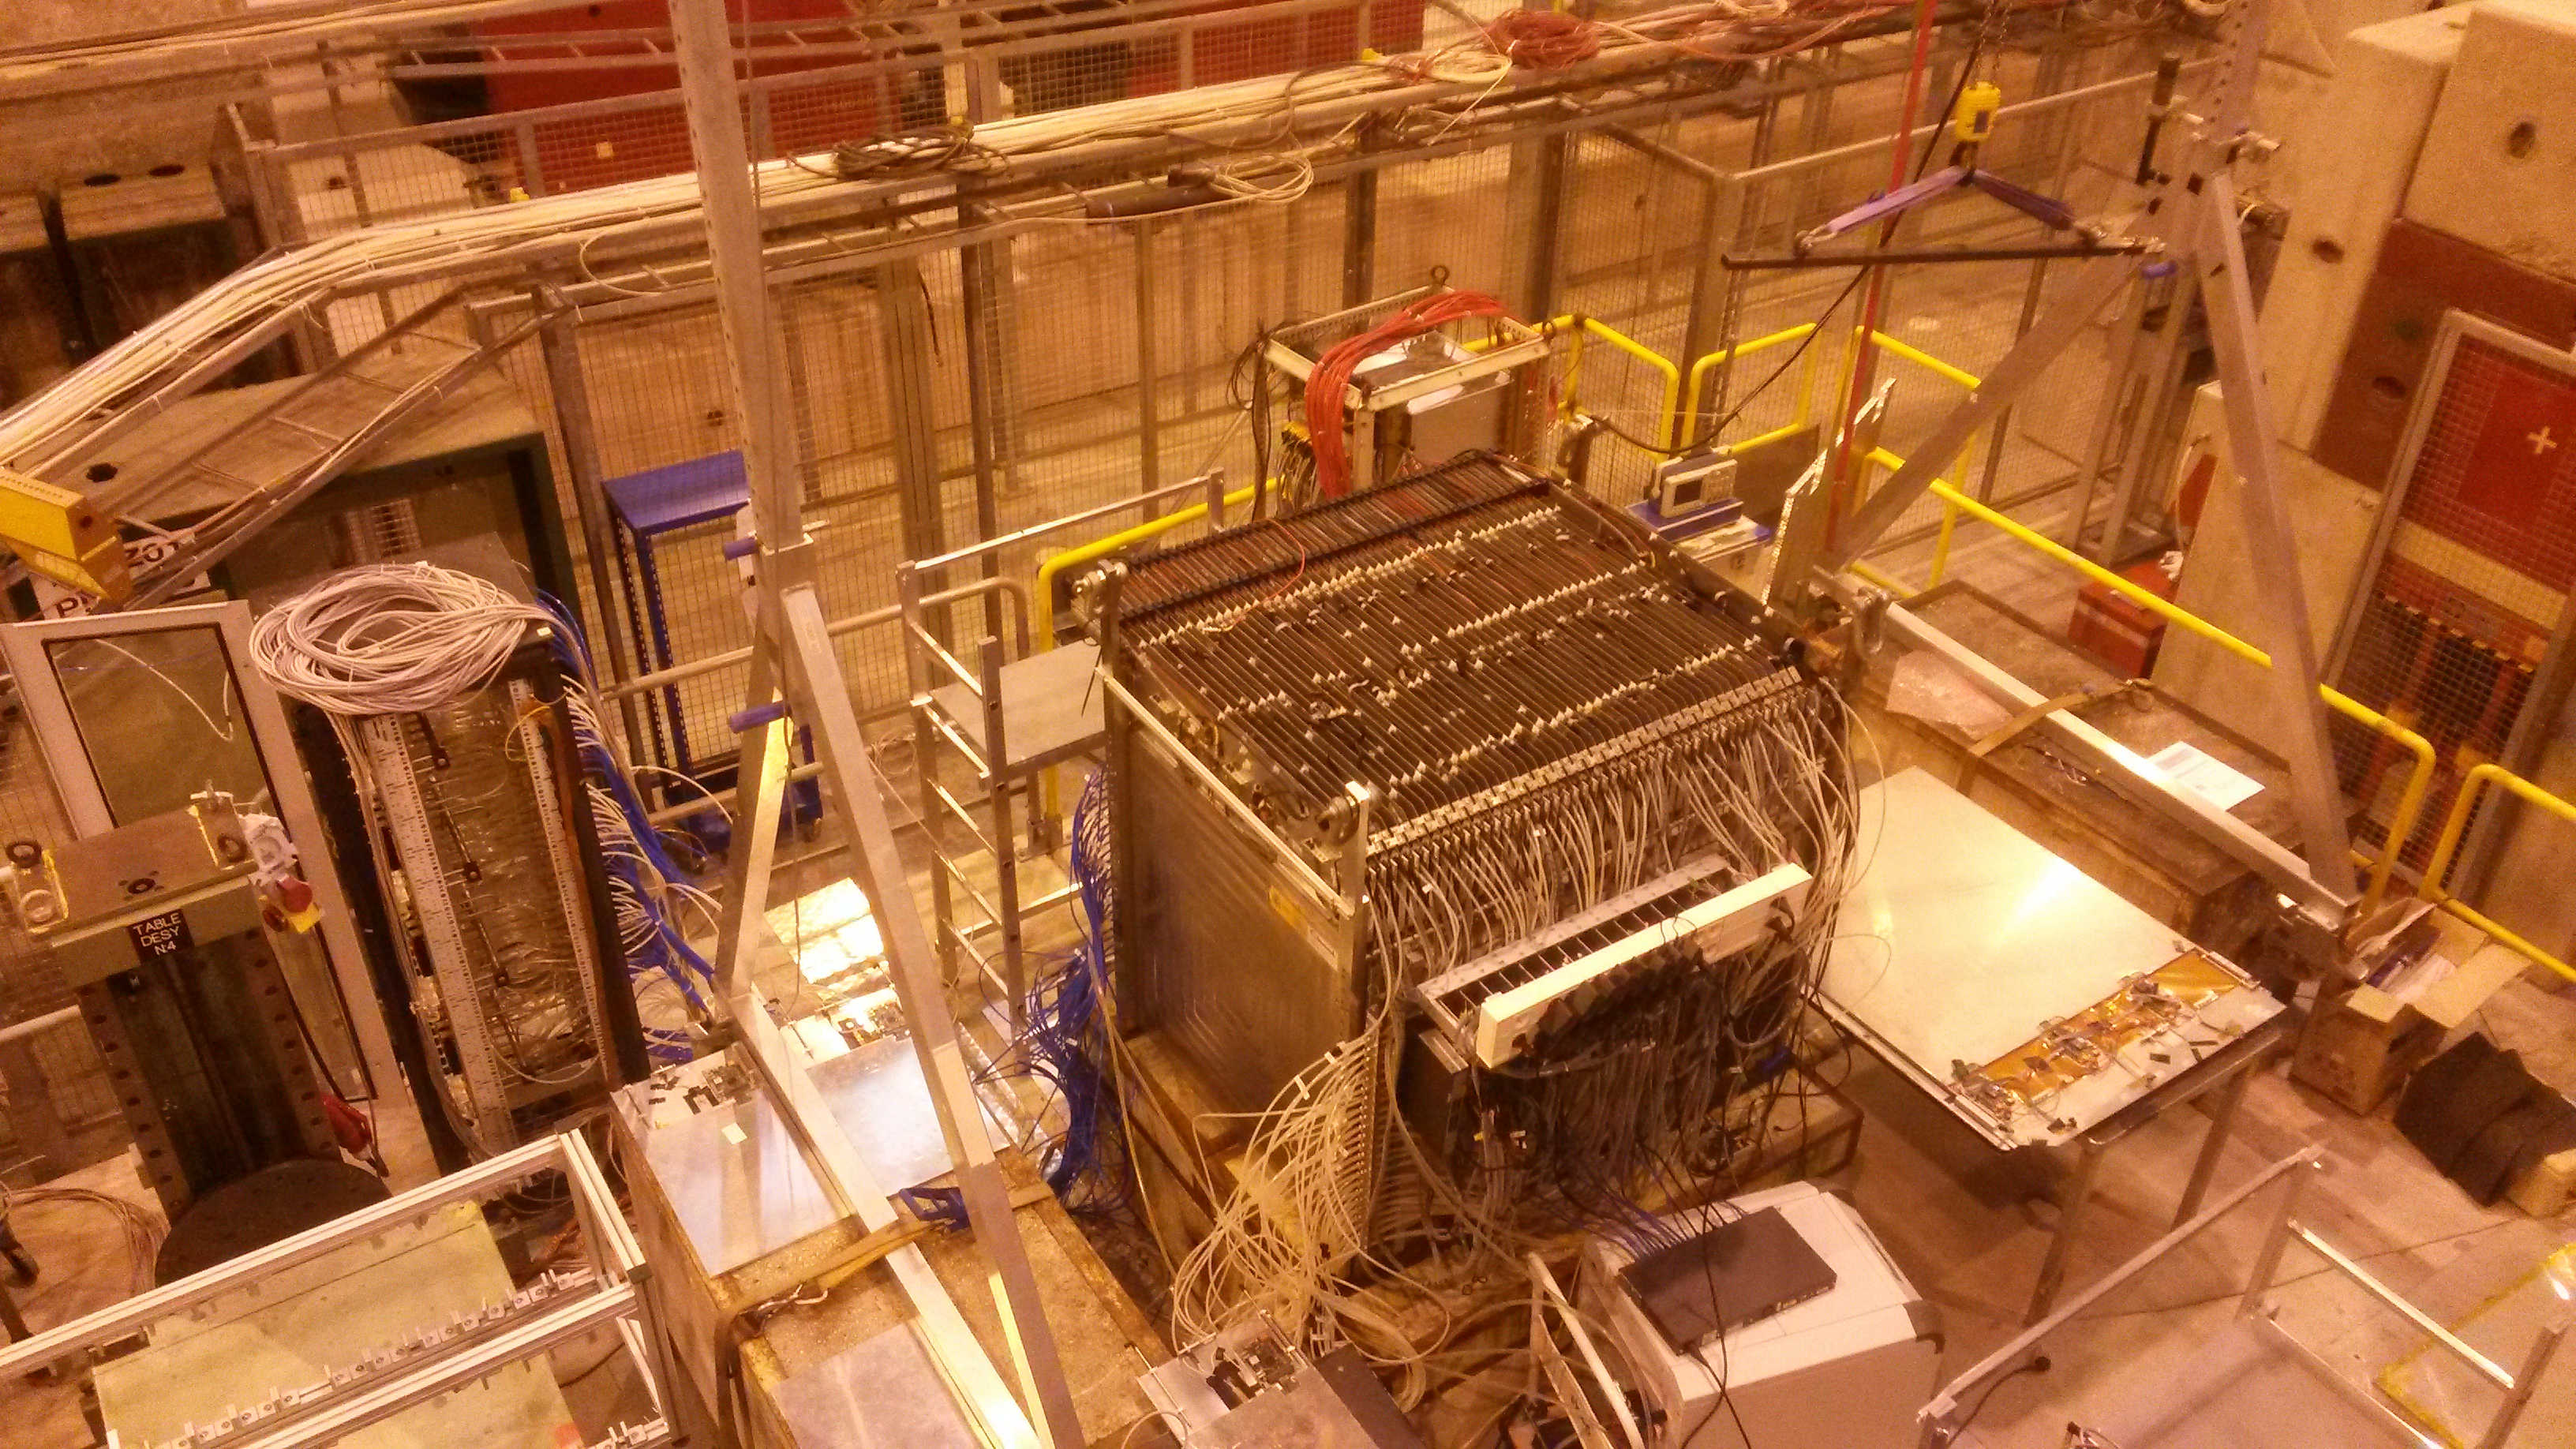
\includegraphics[width=.8\textwidth]{SDHCAL/figs/proto.jpg}
    \caption{Le prototype du calorimètre à lecture semi-digitale sur la ligne de faisceau H6 du CERN.}
    \label{fig:proto}
  \end{center}
\end{figure}
%
Contrairement à la majorité des calorimètres, le SDHCAL n'a pas été optimisé pour obtenir la meilleure résolution en énergie possible. En effet, la résolution en énergie d'un calorimètre est souvent étroitement liée à sa fraction d’échantillonnage. Cette fraction correspond au rapport entre l'énergie déposée par la cascade dans la partie active du détecteur (le mélange de gaz dans les GRPC pour notre détecteur) et l'énergie totale déposée. Cette fraction est presque nulle pour le SDHCAL alors qu'elle peut être égale à 1 dans le cas de calorimètres homogènes où l'absorbeur et le milieu actif sont confondus (exemple: le calorimètre électromagnétique de CMS). Cependant, les deux principales particularités de ce détecteur sont sa granularité et son mode de lecture semi-digital. Chaque GRPC a une segmentation transverse de 1 $cm^2$. Le mode semi-digital signifie que trois seuils sont appliqués sur la charge induite dans les cellules de lecture des GRPC. Ces seuils permettent non pas de mesurer l’énergie déposée dans le détecteur, mais d'avoir une idée du nombre de particules secondaires créées dans la cascade et traversant les cellules. Les informations sur les seuils et sur la géométrie de la cascade seront ensuite utilisées pour mesurer l'énergie des particules incidentes. La figure~\ref{fig:shower80} montre le développement d'une gerbe hadronique de 80 GeV dans les plans (xOz) et (yOz), l'axe $Oz$ étant l'axe du faisceau. Cet événement a été enregistré sur la ligne H6 du SPS au CERN lors d'une campagne de tests sur faisceau.
\begin{figure}[!ht]
  \begin{center}
    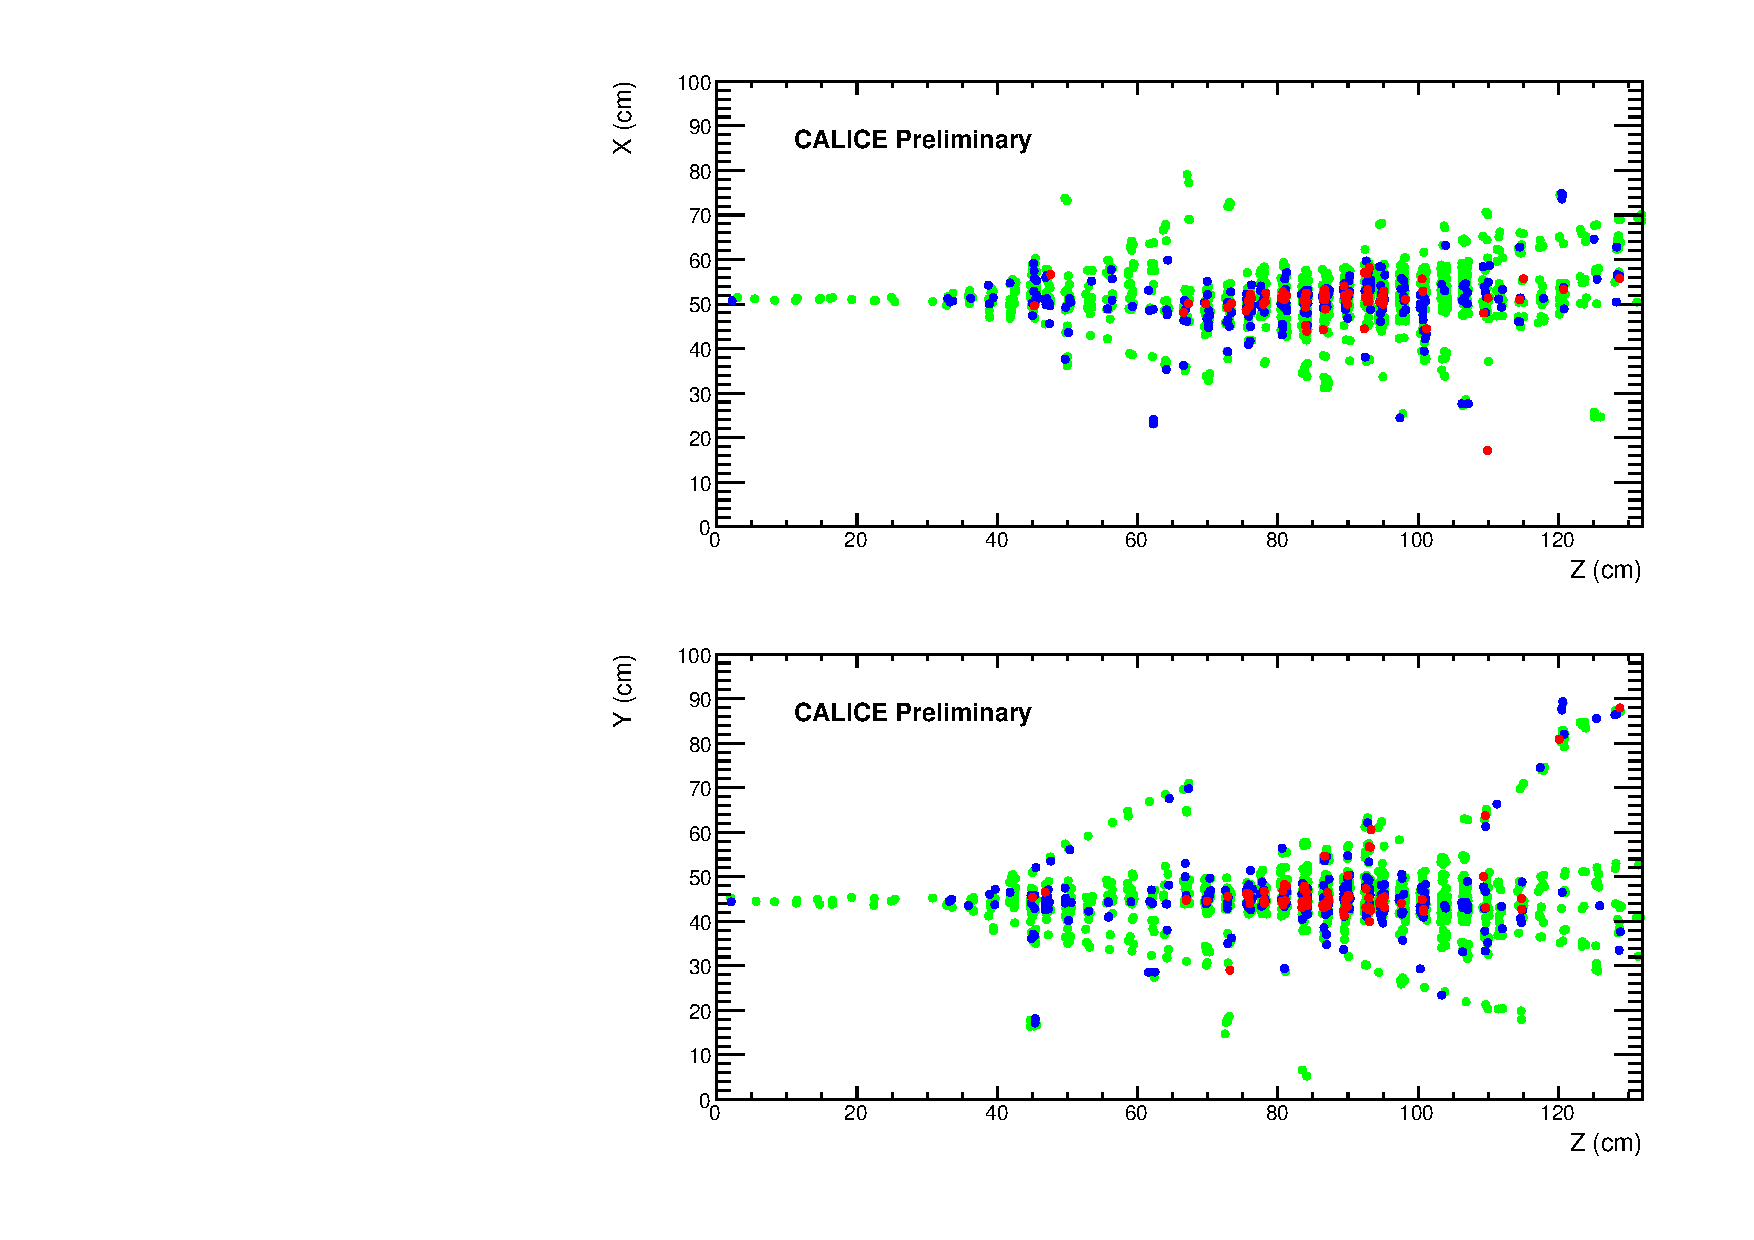
\includegraphics[width=.8\textwidth]{SDHCAL/figs/pion80GeV.pdf}
    \caption{Exemple de gerbe hadronique induite par un pion de 80 GeV, enregistré par le prototype du SDHCAL sur la ligne H6 du SPS au CERN. Les couleurs correspondent aux différents seuils de lecture.}
    \label{fig:shower80}
  \end{center}
\end{figure}
Les points verts, bleus et rouges correspondent aux hits enregistrés avec les seuils 1, 2 et 3 respectivement. On constate que les hits associés aux deux seuils supérieurs sont majoritairement situés au centre de la cascade où la densité de particules secondaires est théoriquement la plus importante. Nous verrons par la suite comment les informations relatives aux trois seuils nous aident à améliorer les performances du détecteur. De plus, sur la figure~\ref{fig:shower80} on distingue des branches où aucune nouvelle particule secondaire n'est créée. Cette reconstruction fera l'objet d'une étude dédiée dans le chapite~\ref{chap.topo}. La reconstruction de ces branches est utilisée lors de l'identification des particules dans le prototype (cf. section~\ref{sec.pi_selection}). Elle est aussi utilisée pour améliorer la mesure de l'énergie des gerbes hadroniques.
%%%%%%%%%%%%%%%%%%%%%%%%%%%%%%%%%%%%%%%%%%%%%%%

\section{Les chambres à plaques résistives de verre}
\label{sec.grpc}
%Nous allons maintenant décrire les chambres à plaques résistives de verre utilisées comme partie active du SDHCAL. 
Une chambre à plaque résistive RPC (Resistive Plate Chamber) est un détecteur gazeux composé de deux électrodes construites avec un matériau dont la résistivité varie entre $10^9$ et $10^{12}~\Omega cm$. Ces électrodes sont séparées par une fine couche de gaz allant jusqu'à quelques millimètres. Une peinture conductrice sur la face externe de ces électrodes permet d'appliquer une haute tension. Le gaz est souvent un mélange fait à base de tétrafluoroéthilène (TFE) et d'hexafluorure de soufre (SF6) et de dioxyde de carbone ($CO_2$) ou de l'isobutane ($C_4H_{10}$). Ainsi lorsqu'une particule chargée traverse la couche de gaz, quelques molécules de gaz sont ionisées. Les électrons et les ions ainsi créés, sont accélérés par le fort champ électrique généré par la haute tension puis ionisent à leur tour d'autres molécules. Une cascade électronique, et une autre ionique, sont alors créées. Ces charges migrent vers les électrodes et induisent un courant sur des canaux de lecture (carreaux, pistes de cuivre).

Selon la valeur de haute tension appliquée et la composition du mélange de gaz, on peut différencier plusieurs modes de fonctionnement des RPC. Le premier mode obtenu, lorsqu'on augmente la tension, est le mode avalanche. Dans ce mode, le gain sur le nombre d'électrons générés par l'avalanche, est limité et le temps nécessaire pour neutraliser les charges déposées sur les électrodes est de quelques dizaines de millisecondes. Ce mode permet de détecter des particules sous des fréquences relativement élevées car le temps de neutralisation est assez court. En continuant d'augmenter la tension, on passe progressivement au mode $streamer$. Dans ce mode, la quantité de charges déposées sur les électrodes est beaucoup plus importante. Ainsi, le temps de neutralisation des charges sera plus long et ne permettra pas de travailler avec des fréquences de détection très élevées.

Les RPC permettent d'obtenir une bonne résolution spatiale et une résolution temporelle de l'ordre de 1 $ns$ avec une épaisseur de la couche de gaz de 2 $mm$~\cite{riegler}. Il est aussi possible d'obtenir de meilleures résolutions temporelles avec des couches de gaz plus fines. Les RPC sont utilisées comme détecteur de muons dans les expériences ATLAS~\cite{atlas} et CMS~\cite{cms}. Pour ces deux expériences, les électrodes sont en bakélite. Ce matériau a une résistivité électrique volumique de l'ordre de $\rho\simeq10^{10}~\Omega cm$. La résistivité volumique des électrodes est un paramètre très important pour les RPC. En effet, les charges positives et négatives issues de la cascade qui sont déposées sur les électrodes, écrantent le champ électrique et celui-ci chute localement dans la couche de gaz. Ainsi le détecteur sera aveugle pendant un certain temps dans la région de la cascade. La résistivité de la bakélite lui permet d'être très efficace sous un flux de particules allant jusqu'à quelques centaines de $Hz/cm^2$. Cependant, l'utilisation de la bakélite entraîne quelques difficultés de réalisation et de maintenance. Il est techniquement difficile de construire des plaques de bakélite de très faible épaisseur ($<1~mm$) avec une surface uniforme. Or le calorimètre de l'ILD qui sera installé à l'intérieur de l'aimant doit être le plus compact possible. De l'huile de lin humidifiée est souvent déposée sur les électrodes pour assurer l'uniformité de surface et donc du champ électrique dans la couche de gaz. Cette huile de lin peut être une source d'ennui. Les RPC des chambres à muons de l'expérience BaBar ont rencontré plusieurs problèmes \cite{vavra}: 
\begin{itemize}
\item l'huile de lin s'est échappée des zones actives à cause de la température (30-35$°C$);
\item des gouttes d'huile de lin se sont formées et étaient responsables de claquages dans les chambres;
\item les forces électrostatiques agissant sur l'huile de lin humidifié ont détérioré la surface des électrodes.
\end{itemize}
Ainsi, les RPC des chambres à muons de l'expérience BaBar ont vu leur efficacité de détection sensiblement dégradée avec le temps \cite{1352718}. 

L'utilisation de matériaux plus résistifs permet de diminuer le bruit dans les RPC, ce qui sera utile pour l'ILC où aucun système de déclenchement extérieur ne sera utilisé. C'est pourquoi le verre a été choisi pour les électrodes du SDHCAL. De plus, l'utilisation du verre permet d'obtenir de larges surfaces très homogènes sans avoir à utiliser un traitement supplémentaire (huile de lin). Cependant, la résistivité du verre ne nous permet pas d'utiliser le SDHCAL sous un flux très élevé de particules (cf. section~\ref{sec.timeCalib} de ce chapitre). 

\subsection{Description des GRPC utilisées dans le SDHCAL}
 %Pour le SDHCAL, le verre a été choisi pour les électrodes. 
La résistivité électrique volumique du verre choisi pour le SDHCAL est $\rho=10^{12}~\Omega cm$. La figure~\ref{fig:grpc} présente un schéma des GRPC utilisées pour le prototype du SDHCAL \cite{kieffer}. 
\begin{figure}[!ht]
  \begin{center}
    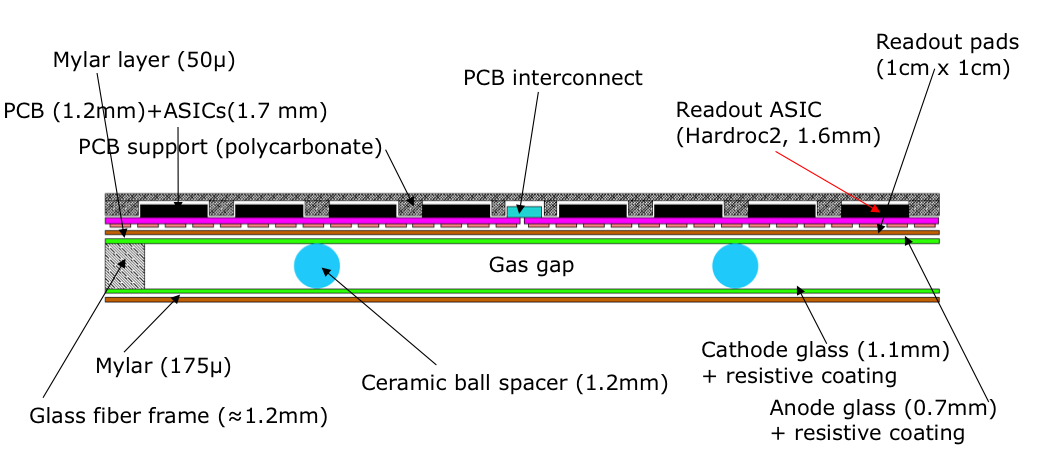
\includegraphics[width=.8\textwidth]{SDHCAL/figs/GRPC-K7.png}
    \caption{Schéma descriptif d'une chambre à plaque de verre résistif utilisée dans le SDHCAL.}
    \label{fig:grpc}
  \end{center}
\end{figure}
L'anode et la cathode ont des épaisseurs de 0.7 et 1.1 $mm$ respectivement. La peinture appliquée sur ces électrodes est une peinture, constituée de 2 composants à base de graphite colloïdal. Les électrodes sont séparées d'une distance de 1.2 $mm$ dans laquelle circule le gaz. Cette distance est garantie par des billes en céramique de 1.2 $mm$ de diamètre collées entre les électrodes. Des carreaux capacitifs en cuivre de 1 $cm^2$ (figure~\ref{fig:carreaux}), sont utilisés pour collecter la charge. Ils sont directement imprimés sur une face du circuit de lecture. Chaque GRPC de 1 $m^2$ contient 9216 carreaux de cuivre, ce qui conduit à plus de de 440000 canaux de lecture pour le prototype.
\begin{figure}[!ht]
  \begin{center}
    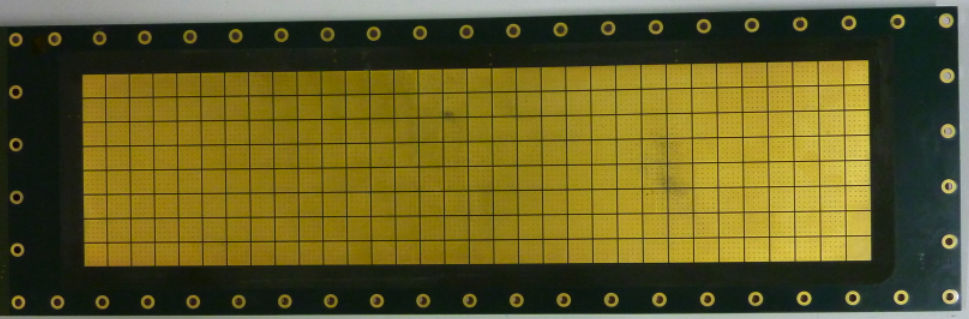
\includegraphics[width=.8\textwidth]{SDHCAL/figs/PADs.png}
    \caption{Les carreaux de cuivres capacitifs de 1 $cm^2$ imprimés de l'autre coté du circuit de lecture d'une petite chambre utilisée pendant le développement du détecteur.}
    \label{fig:carreaux}
  \end{center}
\end{figure}
Une feuille de Mylar de 50 $\mu m$ est déposée entre l'anode et les carreaux de cuivre pour isoler ces derniers. Le circuit imprimé PCB (Printed Circuit Board) est composé de 6 ASUs (Active Sensor Unit) soudés entre eux. Sur chaque ASU, 24 ASIC (Application Specifique Integrated Circuit) HARDROC2~\cite{omega} sont intégrés (figure~\ref{fig:layer}(b)). 
\begin{figure}[!ht]
  \begin{center}
    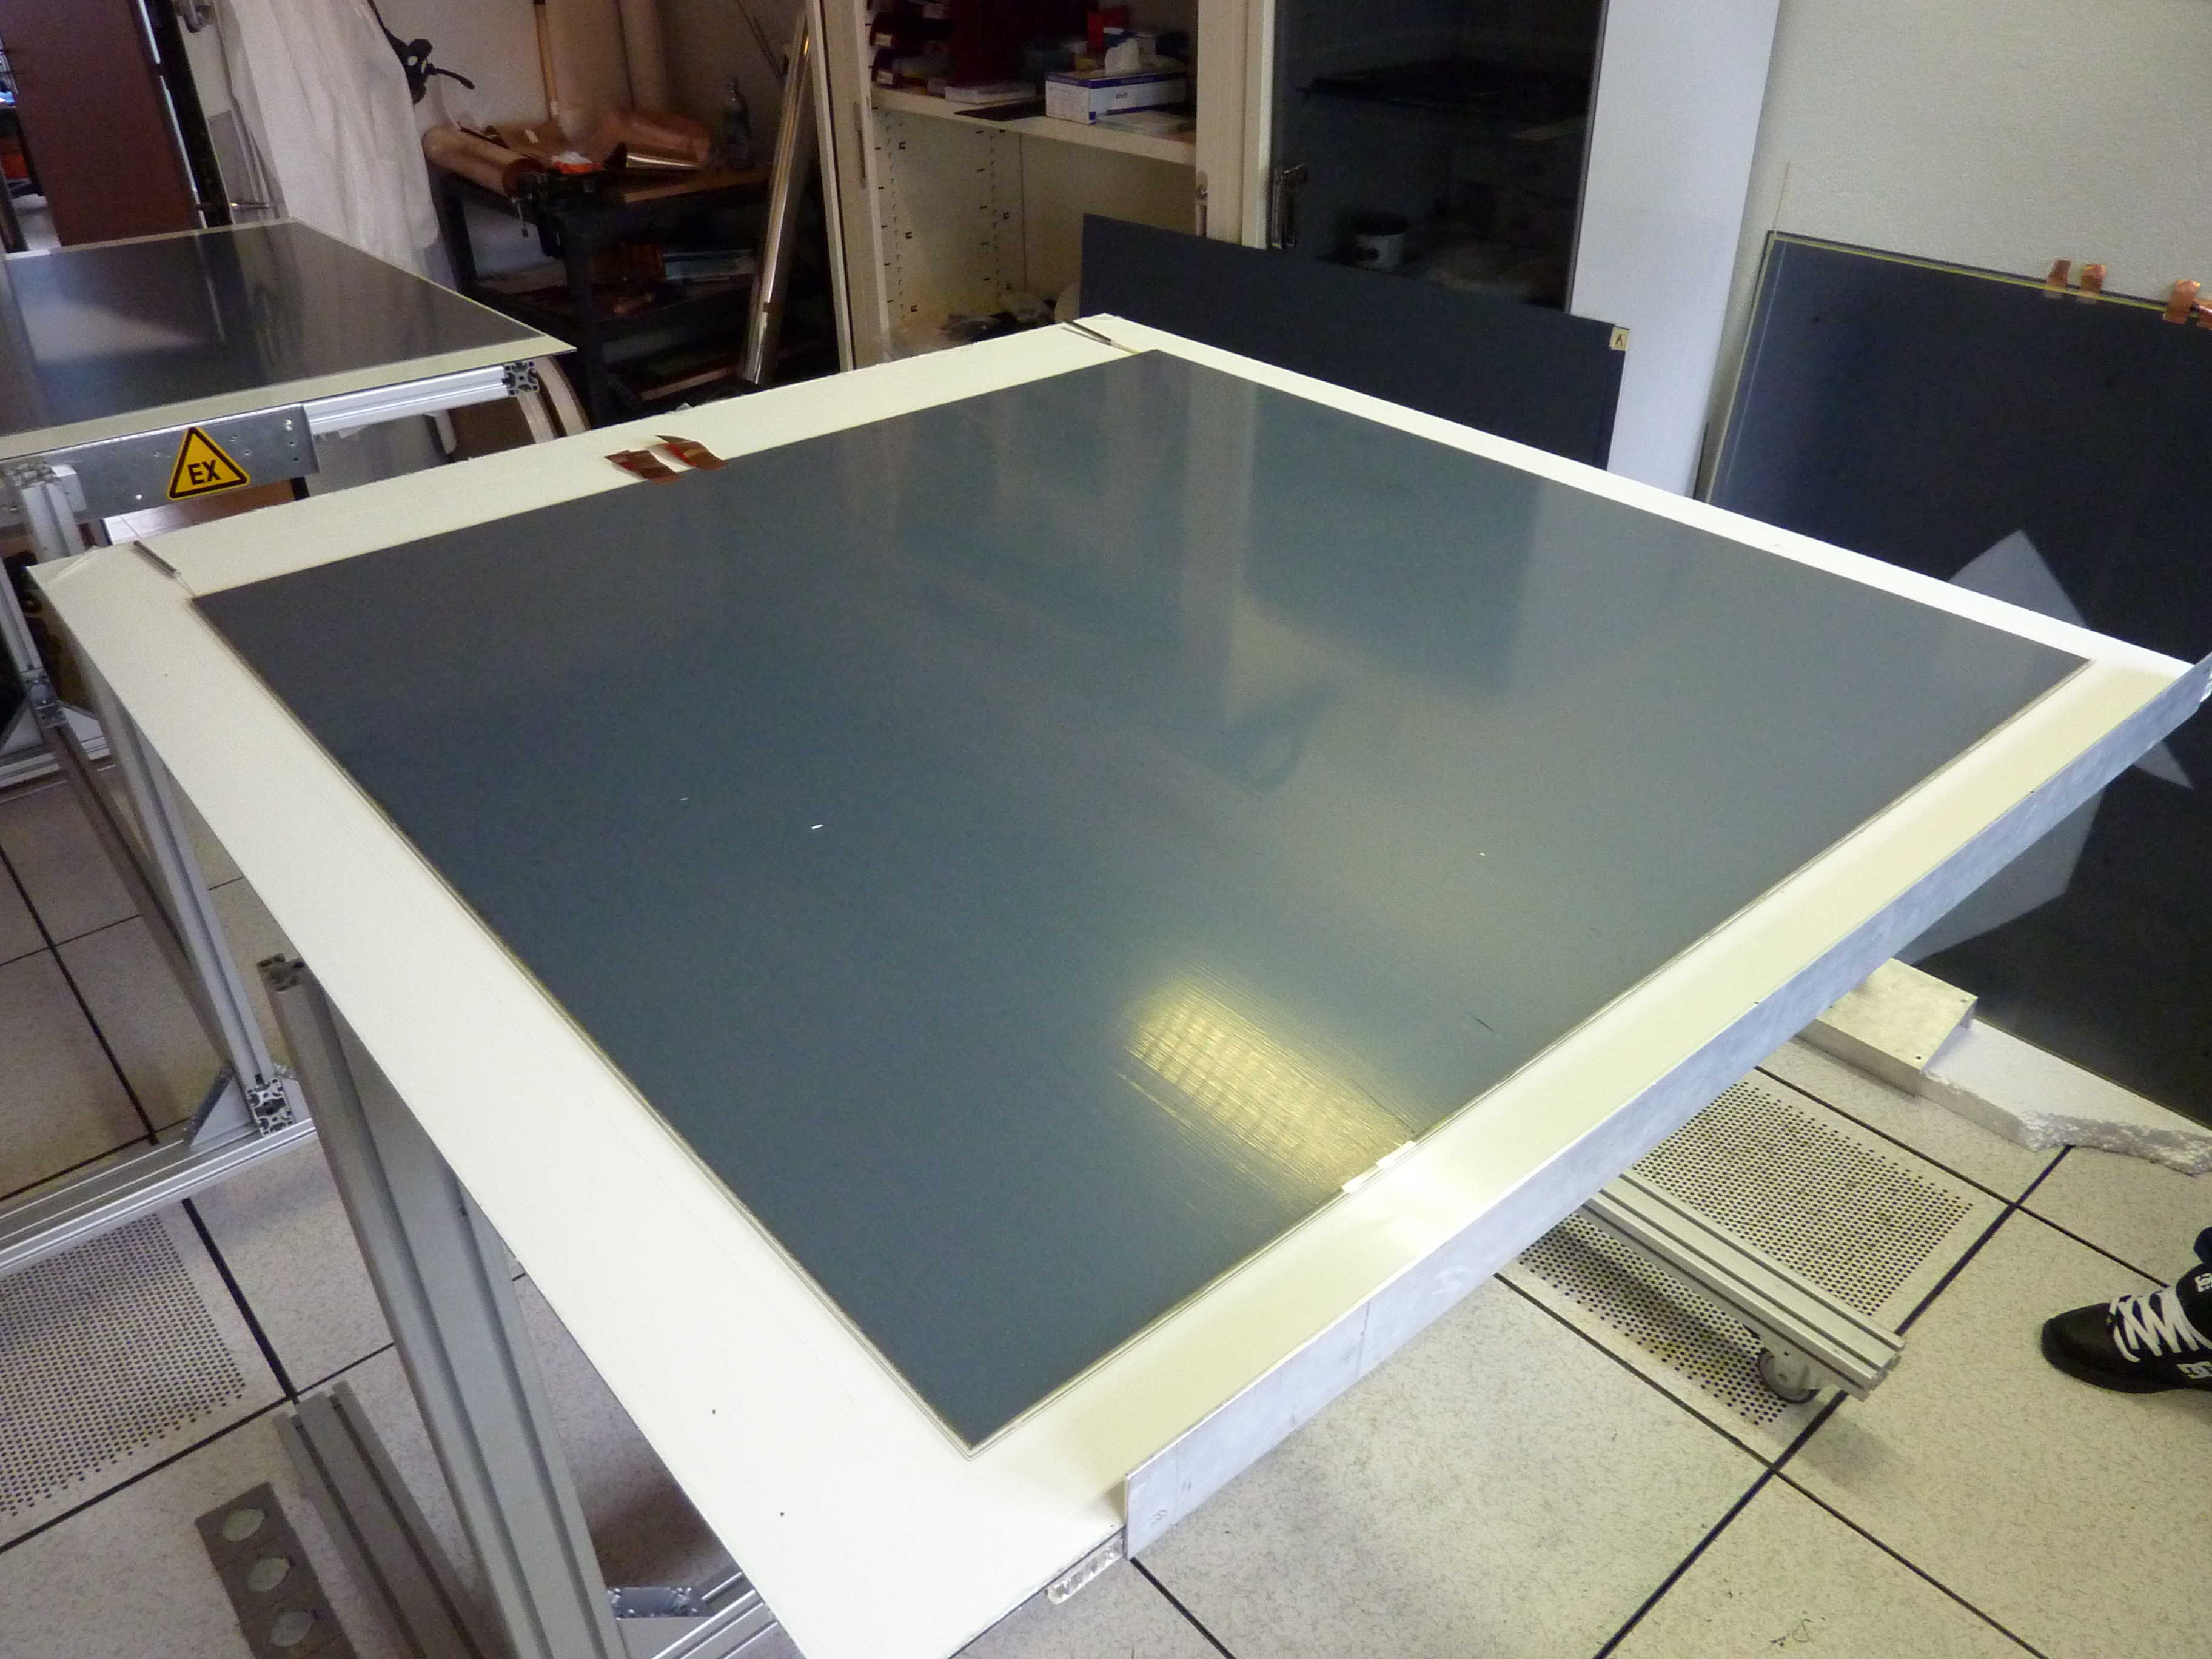
\includegraphics[width=.47\textwidth]{SDHCAL/figs/aLayer.jpg}
    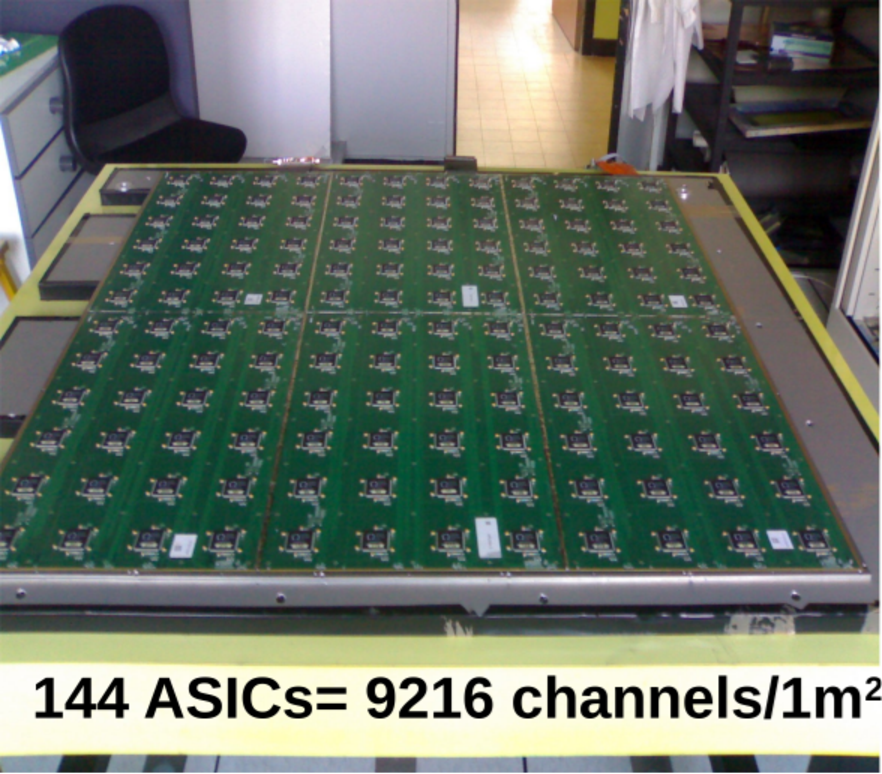
\includegraphics[width=.4\textwidth]{SDHCAL/figs/layer_electronic2.pdf}
    \caption{Photographie d'une GRPC sans son électronique ni sa cassette (à gauche) et d'un circuit imprimé (à droite) sur lequel on distingue les 144 ASIC.}
    \label{fig:layer}
  \end{center}
\end{figure}
Chacun de ces ASIC est relié à 64 carreaux de cuivre. Ces ASIC collectent les signaux des carreaux de cuivre, puis ces signaux sont mis en forme et trois discriminateurs en font l'analyse pour déterminer le seuil franchi par les signaux. Trois cartes interfaces détecteur DIF (Detector InterFace) par GRPC font le lien entre les ASIC et les ordinateurs d'acquisition. Les paramètres de l'acquisition (valeurs des seuils, des gains...) sont envoyés aux ASIC à travers ces DIF. La figure~\ref{fig:DIF} montre une photographie du haut d'une GRPC avec ses trois DIF connectées au PCB.
\begin{figure}[!ht]
  \begin{center}
    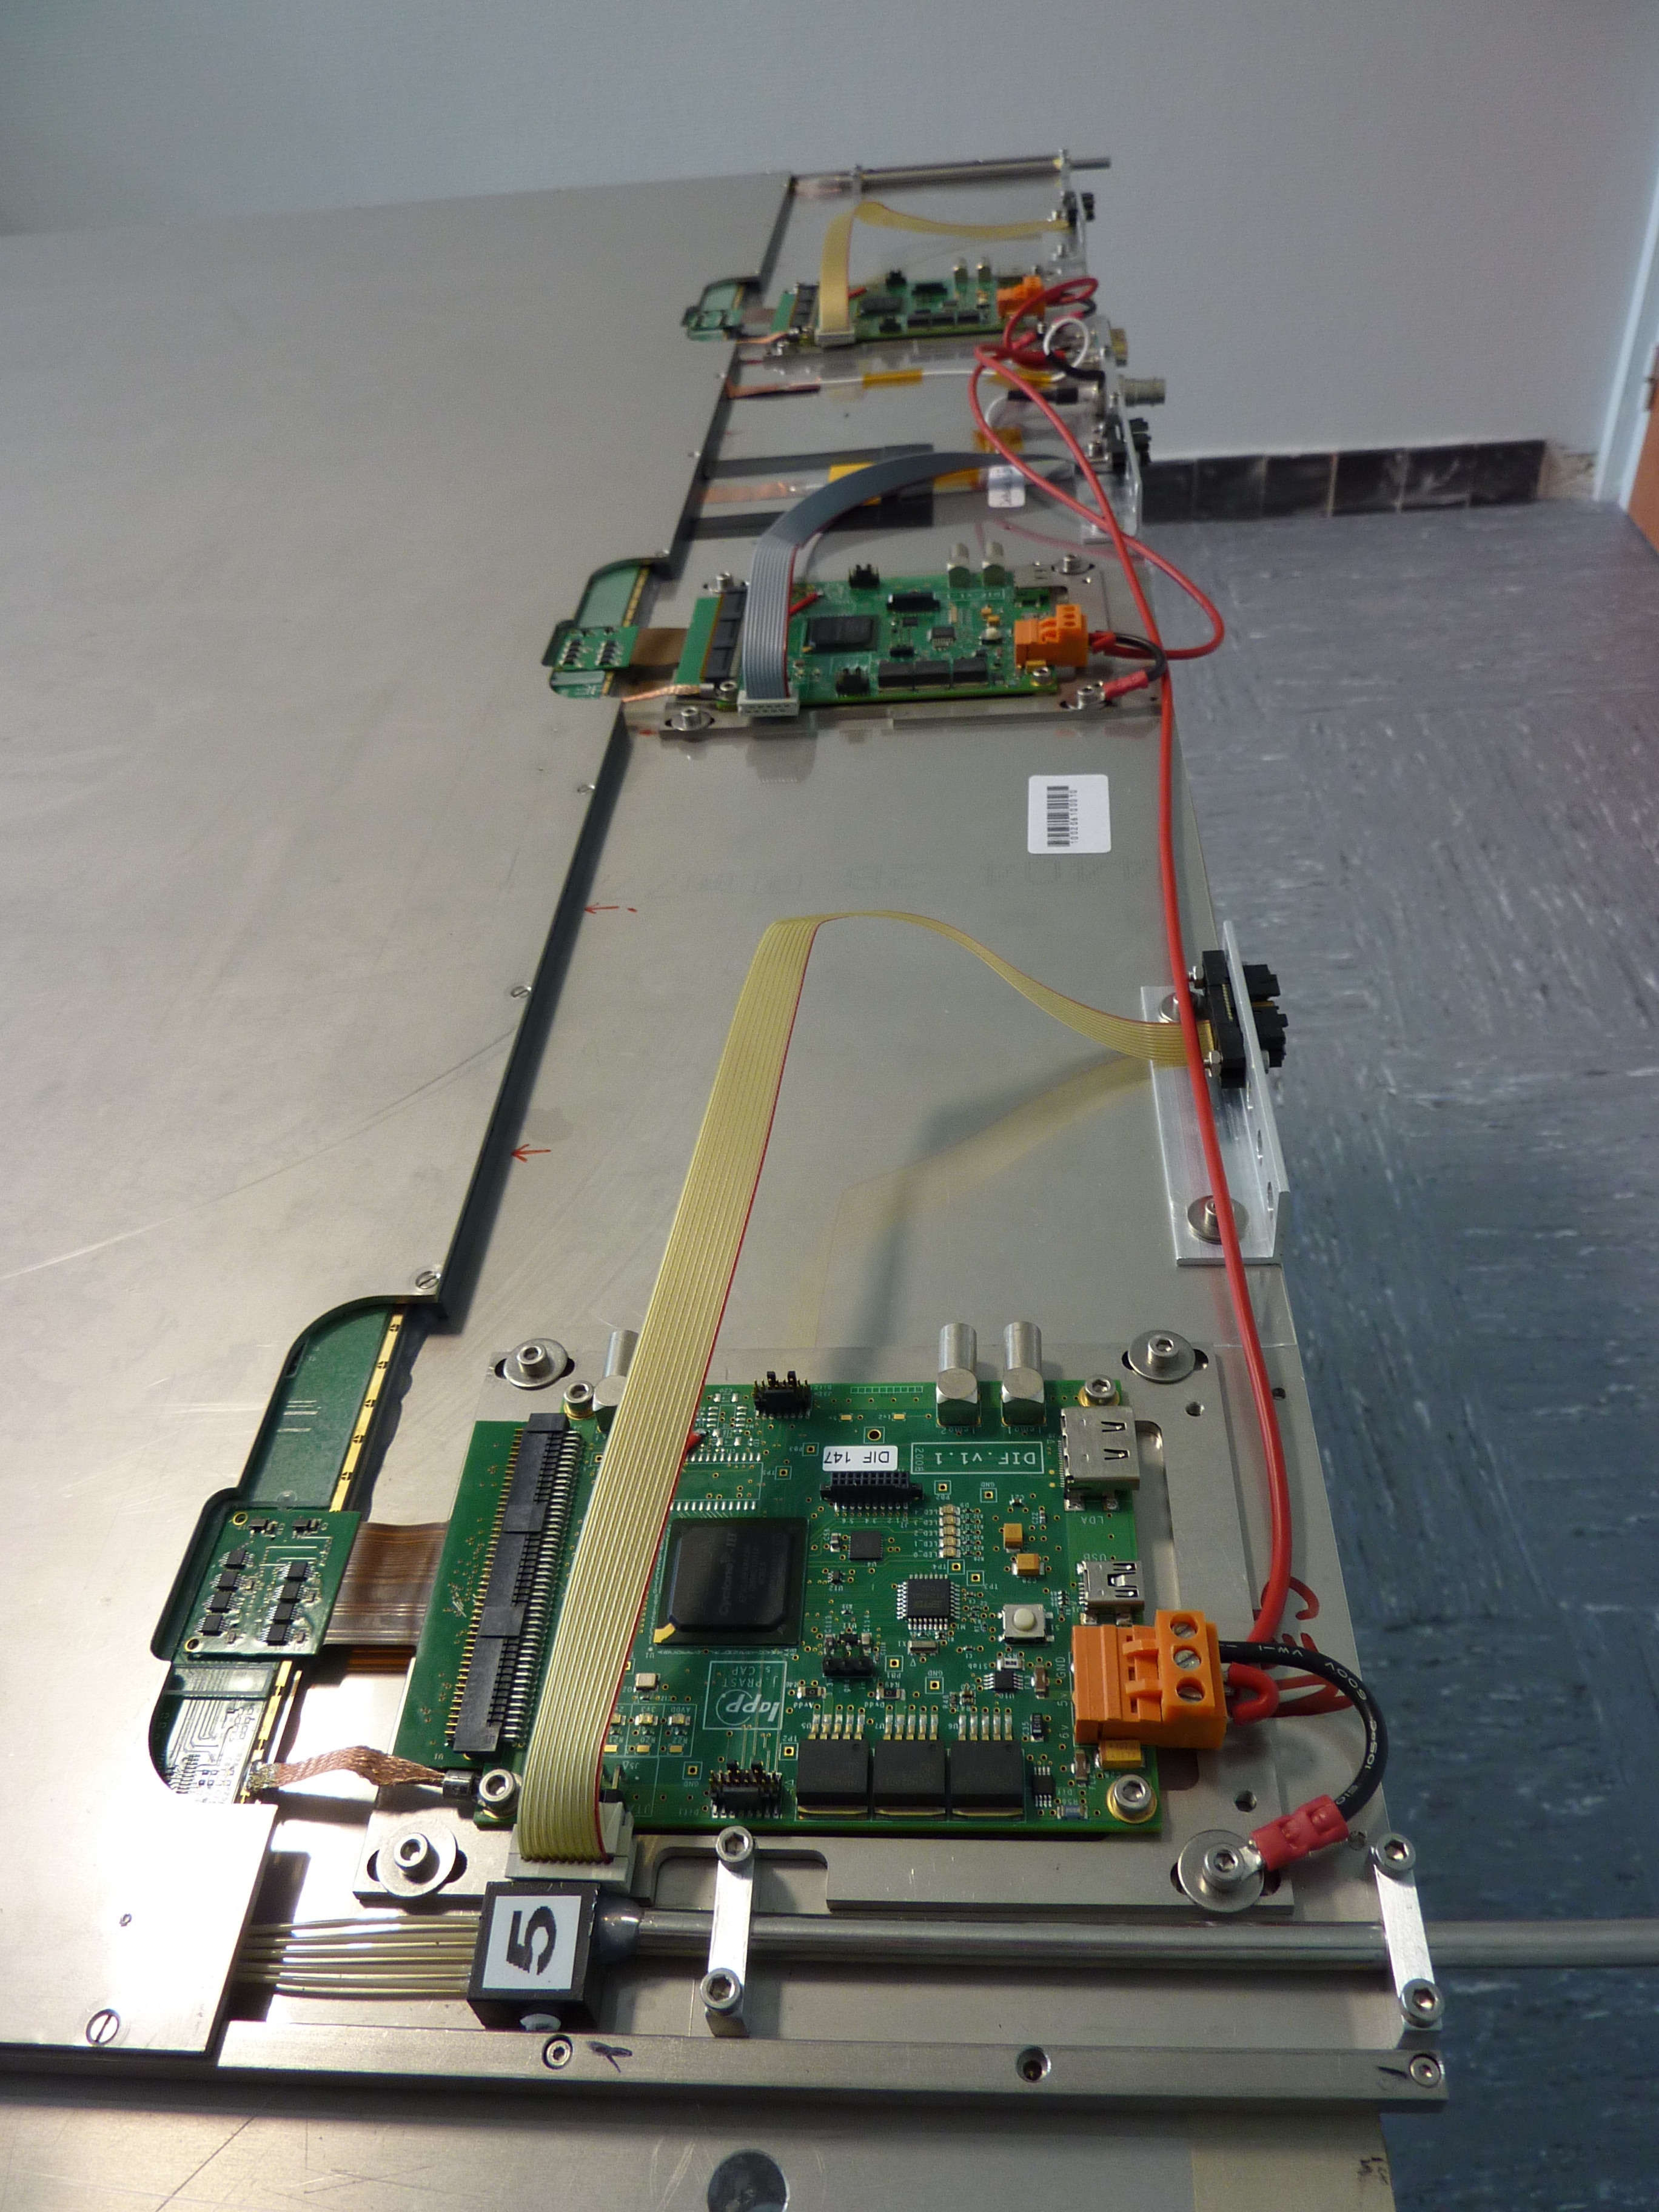
\includegraphics[width=.4\textwidth,angle=90]{SDHCAL/figs/DIFCassette.jpg}
    \caption{Photographie du haut d'une cassette avec ses trois DIF connectées au PCB.}
    \label{fig:DIF}
  \end{center}
\end{figure}

\subsection{Alimentation pulsée}
Le prototype du SDHCAL possède déjà plus de 440000 canaux de lecture. Le calorimètre hadronique final d'une expérience telle que l'ILD comportera plus de 70 millions de cellules de 1 $cm^2$. L'énergie dissipée avec des cellules de lecture classiques sera telle que l'utilisation de systèmes de refroidissement deviendrait indispensable. Or ces systèmes auraient un budget matière non négligeable, ce qui dégraderait la résolution en énergie des jets. De plus pour utiliser des techniques de suivi des particules dans tous les sous-détecteurs, il faut minimiser les zones non instrumentées. Cependant, le système d'accélérateur à l'ILC ne délivrera du faisceau que pendant 0.95 $ms$ toute le 200 $ms$ \cite{acceleratorTDR}. La figure~\ref{fig:ILCCycle} montre un schéma de la structure temporelle du faisceau de l'ILC.
\begin{figure}[!ht]
  \begin{center}
    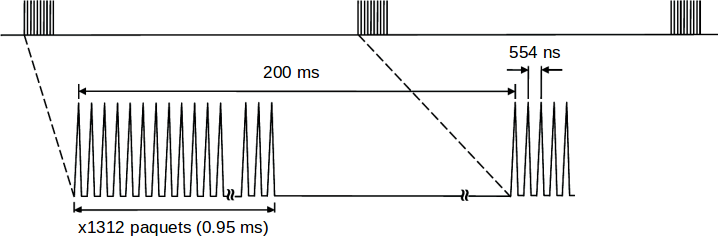
\includegraphics[width=.8\textwidth]{SDHCAL/figs/PPCycle.png}
    \caption{Schéma de la structure temporelle du faisceau de l'ILC.}
    \label{fig:ILCCycle}
  \end{center}
\end{figure}
Cette structure temporelle permettra de lire les données du détecteur entre deux croisements de faisceaux. De plus, ce mode de fonctionnement permet d'utiliser une alimentation pulsée pour les sous-détecteurs. Certains composants des détecteurs ne seront allumés que pendant les collisions entre particules ($\Delta_t=0.95~ms$). Cela permettra de diminuer sensiblement la consomation des détecteurs, ce qui entraînera une forte réduction de la dissipation thermique et par conséquent du bruit dans les détecteurs. Le prototype du SDHCAL a été le premier détecteur utilisant une alimentation pulsée après avoir testé le fonctionnement d'une chambre GRPC en mode pulsée dans un champ magnétique \cite{pp-in-mag-field}. Lors des tests en faisceau, au SPS en 2012, les particules étaient délivrées par l'accélérateur pendant 9 $s$ toutes les 45 $s$. Ainsi, les composants analogiques des ASIC qui sont les composants ayant la plus forte consommation d'énergie, étaient éteints pendant les 34 $s$ sans faisceau. Les caractéristiques du SPS sont différentes des futures caractéristiques du faisceau de l'ILC. Pour opérer le prototype du SDHCAL dans de bonnes conditions un simple système de refroidissement du détecteur a été utilisé. Il est fait de plaques de cuivre fixées aux deux cotés latéraux du prototype, et dans lesquelles circule de l'eau refroidie à 10$\degres C$.

\subsection{Description d'un cycle d'acquisition}
Au début d'une phase d'acquisition, l'horloge interne des ASIC est remise à zéro. Les ASIC et les DIF sont synchronisés à l'aide de DCC (Data Concentrator Card) et d'une SDDC (Synchronous Data Concentrator Card). Le temps dans les ASIC et dans les DIF est échantillonné par pas de 200 $ns$. Pendant une phase d'acquisition, lorsqu'un ou plusieurs des 64 canaux d'un ASIC passe le premier seuil, un événement est stocké dans la mémoire interne de l'ASIC. Chaque HARDROC peut enregistrer jusqu'à 127 événements de ce type. Lorsque la mémoire d'un des ASIC du détecteur est plein, un signal RAMfull est envoyé au pilote de l'acquisition, l'acquisition est stoppée et les mémoires internes de tous les ASIC sont lues par les DIF puis envoyées aux ordinateurs d’acquisition. Un événement RAMfull (la construction des événements physiques sera discutée dans la section~\ref{sec.trivent} de ce chapitre) est alors stocké sur disque. Les informations contenues dans ces événements sont les suivantes: 
\begin{enumerate}[1-]
\item le numéro de l'événement RAMfull;
\item le temps absolu au moment du signal RAMfull (échantillonné par pas de 200 $n$s) depuis le début de la prise de donnée;
\item pour chaque hit:
  \begin{enumerate}[-]
    \item une clef unique permet de retrouver la position du carreau de cuivre. Dans cette clef on retrouve le numéros de la DIF (de 0 à 255), le numéro de l'ASIC (de 0 à 47) et enfin le numéro du canal (de 0 à 63);
    \item le temps (par pas de 200 $n$s) relatif au début du cycle d'acquisition;
    \item le seuil déclenché par le signal induit sur le carreau de cuivre;
  \end{enumerate}
\end{enumerate}
Après cette phase de lecture, un nouveau cycle d'acquisition démarre automatiquement. Ce mode d'acquisition a la particularité de ne pas utiliser de système de déclenchement externe ({\it{trigger}}). Les données collectées en test faisceau, contiendront donc des événements venant de particules du faisceau, des particules cosmiques et le bruit des détecteurs. Ce bruit est un paramètre important à contrôler. En effet si des canaux électroniques sont trop bruyant, ils seraient responsables de signaux RAMfull déclenchés immédiatement après le début du cycle et empêcheraient donc l'enregistrement de données. La haute résistivité électrique du verre permet de limiter ce bruit. Ce mode de lecture sans déclenchement externe, rend également obligatoire une procédure de reconstruction des événements dits physiques que nous détaillerons dans la section~\ref{sec.trivent}.
\
\subsection{Le réglage des seuils}
\label{sec.sdhcal_thr}
Pour régler les trois seuils des GRPC, un convertisseur digital-analogique (DAC), encodé sur 10 bits (de 0 à 1023), est utilisé pour chaque seuil. Les facteurs de conversion, donnant la valeur du seuil sur la charge induite à partir de la valeur de DAC, sont déterminés à l'aide de l'injection d'une charge. Un condensateur de capacité 2 $pF$, permet d'injecter une charge donnée sur les 64 canaux des ASIC. Ce dispositif permet d'effectuer un scan sur la charge injectée. Pour chaque valeur de charge injectée, la valeur du seuil de basculement, qui correspond à la valeur de DAC pour laquelle l'efficacité de détection est égale à 50\%, est mesurée \cite{kieffer}. Les courbes de ces valeurs en fonction de la charge injectée sont construites pour chaque canal des ASIC, pour chaque seuil. La figure~\ref{dac-vs-inj} montre un exemple de ces courbes pour les 64 canaux d'un ASIC, pour le premier seuil. 
\begin{figure}[!ht]
  \centering
  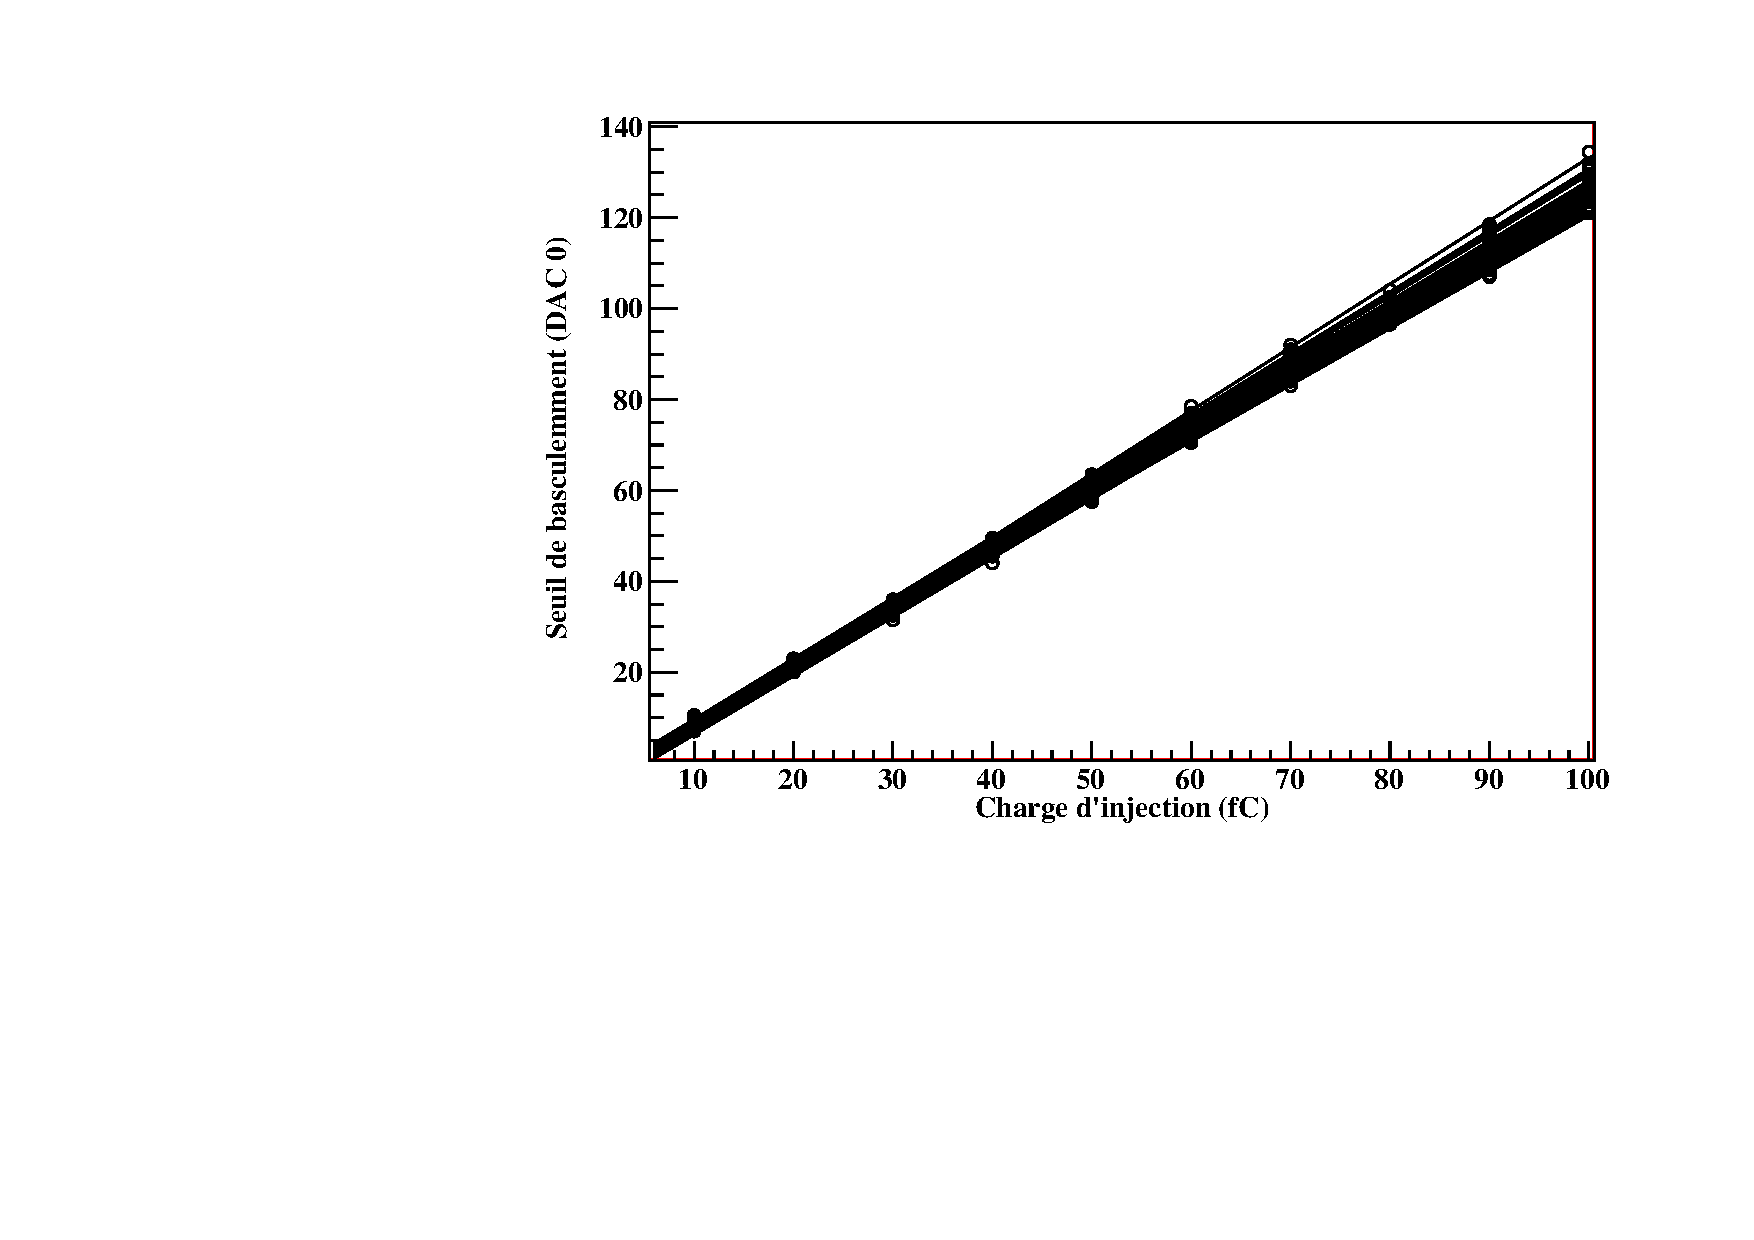
\includegraphics[width=.7\textwidth]{SDHCAL/figs/Dac0Lin.pdf}
  \caption{Seuil de basculement pour le premier seuil ($DAC_0$), en fonction de la charge injectée, pour les 64 canaux d'un ASIC. La valeur du piédestal a été précédemment soustraite.}
  \label{dac-vs-inj}
\end{figure}
La valeur du piédestal a été précédemment soustraite pour la construction de ces courbes. La méthode, pour extraire les valeurs des piédestaux pour chaque seuil, est décrite dans \cite{kieffer}. Les courbes de la figure~\ref{dac-vs-inj} sont ajustées avec une fonction linéaire. Finalement l'équation suivante permet d'obtenir la valeur du seuil en fonction de la valeur de DAC pour chaque seuil:
\begin{equation}
  seuil_i = \frac{DAC_i-p_i}{\lambda_i} [pC]
  \label{eq.dacConversion}
\end{equation}
où les coefficients $\lambda_i$ sont les valeurs moyennes des coefficients directeurs des droites obtenues après les ajustements linéaires, et $p_i$ les valeurs des piédestaux.
Le tableau~\ref{tab.lambdas} présente les valeurs des facteurs de conversion et des piédestaux pour chaque seuil.
\begin{table}[!ht]
  \begin{center}
    \begin{tabular}{c|c|c}
      \rowcolor{black!20!white}Seuil & $\lambda~[pC^{-1}]$ & Piédestal\\
      \rowcolor{black!5!white}\hline
      \rowcolor{black!5!white}0 & 700.0 & 90\\
      \rowcolor{black!5!white}1 & 80.0 & 98\\
      \rowcolor{black!5!white}2 & 16.3 & 98
    \end{tabular}
  \end{center}  
  \caption{Facteur de conversion et valeur des piédestaux pour chaque seuil.}
  \label{tab.lambdas}
\end{table}
Cependant, les courbes permettant d'obtenir les facteurs de conversion (voir figure~\ref{dac-vs-inj}), ne sont pas linéaires sur toute la gamme. Ceci est particulièrement visible pour les seuils supérieurs, comme le montre la figure~\ref{dac-vs-inj_12}.
\begin{figure}[!ht]
  \centering
  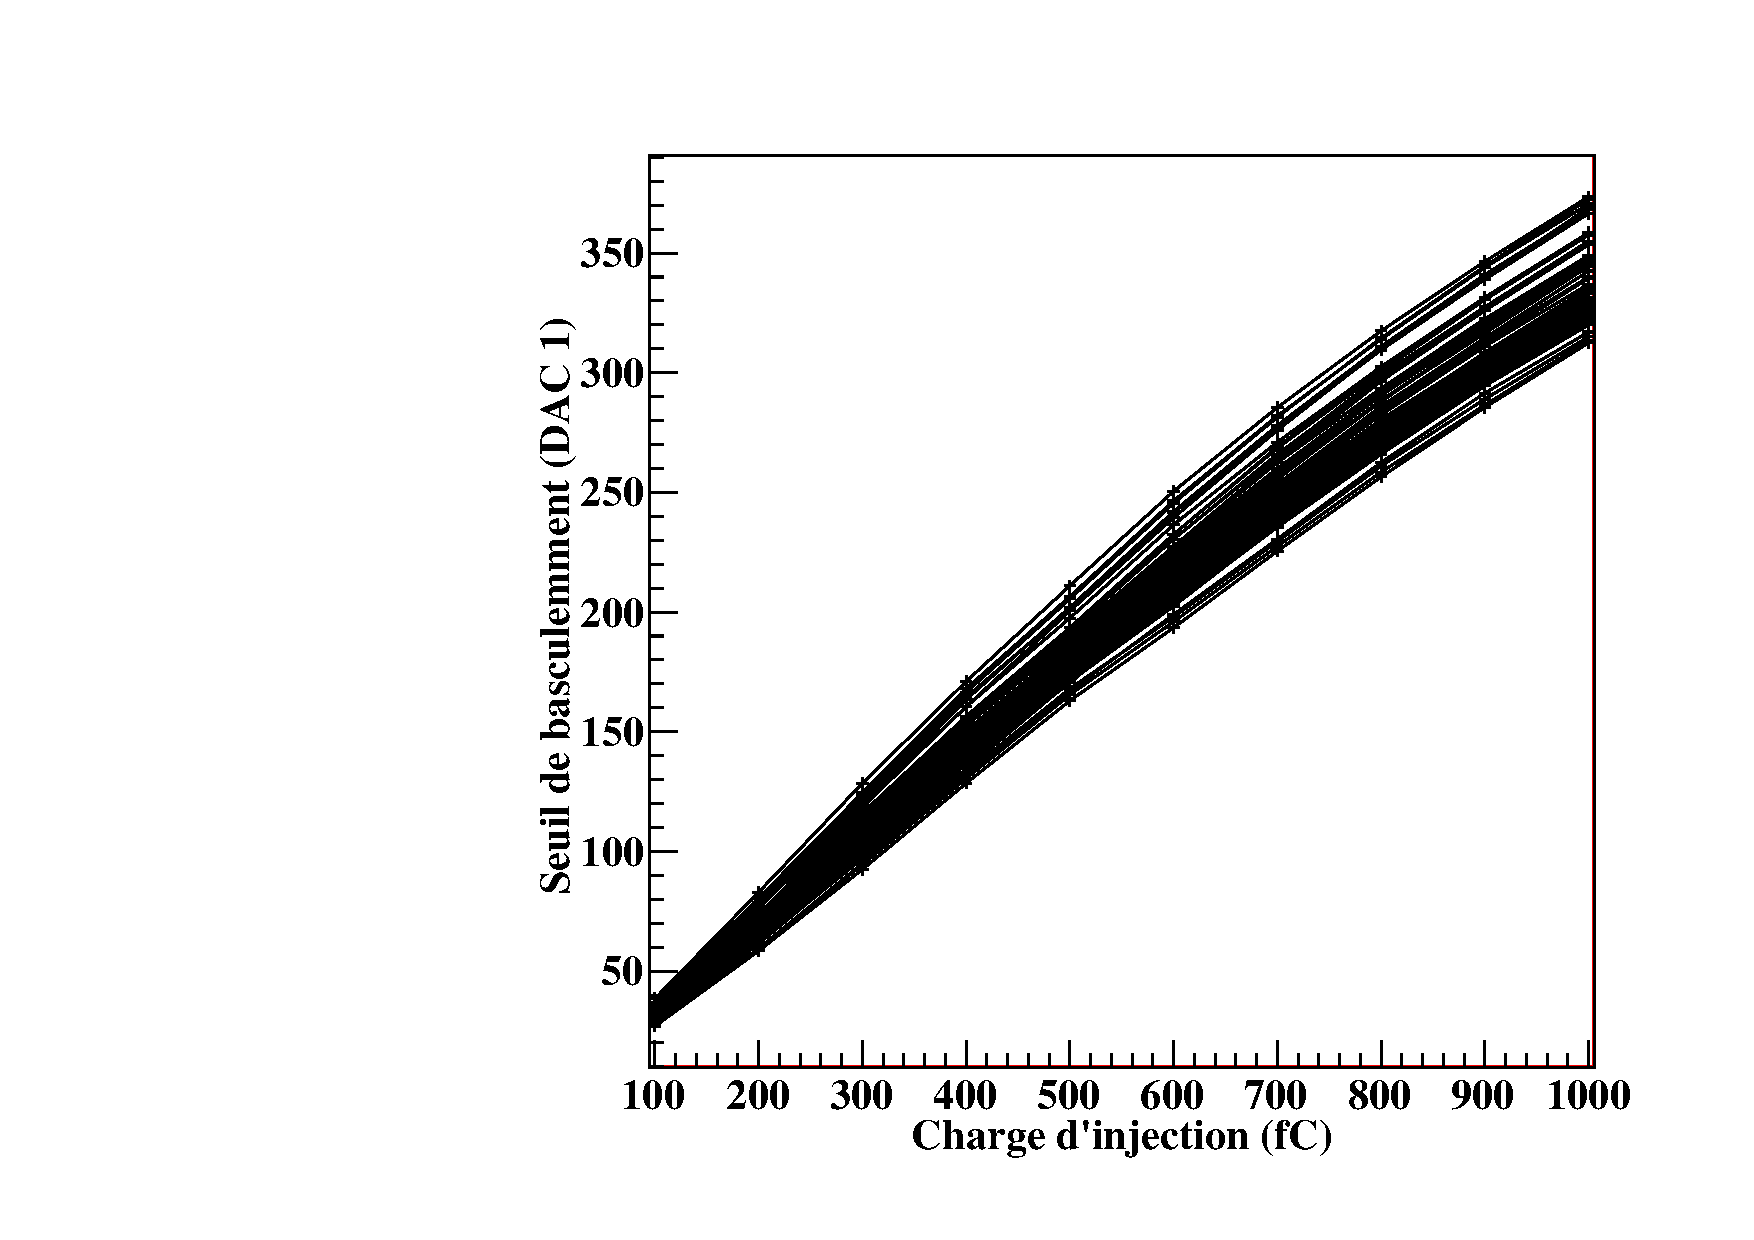
\includegraphics[width=.45\textwidth]{SDHCAL/figs/Dac1Lin.pdf}
  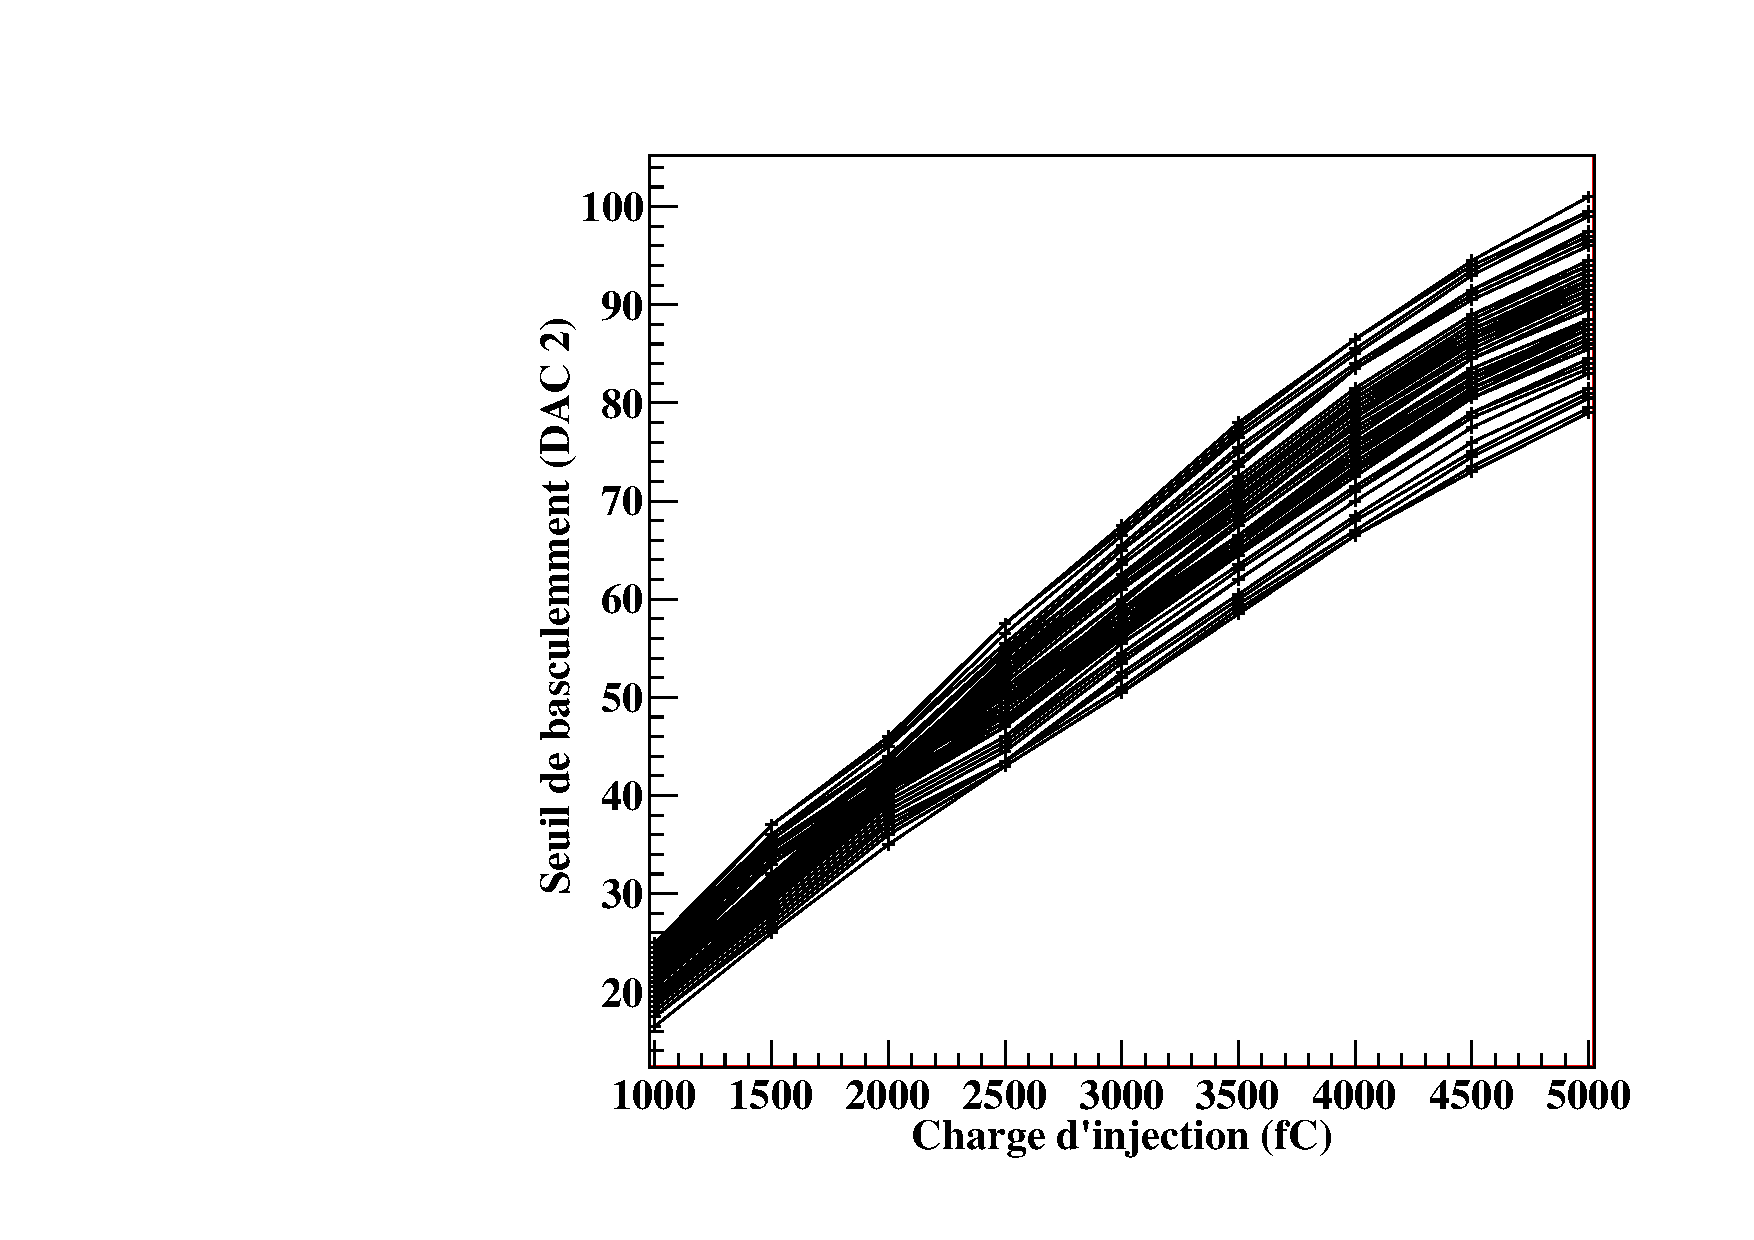
\includegraphics[width=.45\textwidth]{SDHCAL/figs/Dac2Lin.pdf}
  \caption{Seuil de basculement pour le deuxième ($DAC_1$) et troisième ($DAC_2$) seuils en fonction de la charge injectée pour les 64 canaux d'un ASIC. La valeur du piédestal a été précédemment soustraite.}
  \label{dac-vs-inj_12}
\end{figure}
Ainsi, dans le chapitre~\ref{chap.simulation}, pour le réglage des seuils dans la simulation du SDHCAL, nous utiliserons des valeurs de seuils légèrement modifiées par rapport aux valeurs attendues dans le SDHCAL (cf. équation~\ref{eq.dacConversion}).

\subsection{Le fonctionnement d'une GRPC}
Le mode de fonctionnement des GRPC dans le SDHCAL est le mode avalanche. Le mélange gazeux et la haute tension appliquée ont été choisis pour avoir une très bonne efficacité de détection et pour avoir une fréquence de détection raisonnable avec une charge modérée de l'avalanche. 
\subsubsection{Le mélange de gaz}
Le mélange de gaz choisi est le suivant: $93\%$ de $TFE$, $5\%$ de $CO_2$ et $2\%$ de $SF_6$. Le $TFE$ a été choisi pour son faible potentiel d'ionisation (10.7 $eV$). Ce gaz est celui qui fournit les électrons de l'avalanche. Pendant le développement de l'avalanche, certaines molécules sont excitées. Leur désexcitation libère des photons. Ceux-ci risquent d'ioniser d'autres molécules notamment grâce à l'effet photo-électrique et donc de déclencher des avalanches loin de l'endroit de passage de la particule. Le $CO_2$ est utilisé pour limiter cet effet. Le $SF_6$ est un gaz très électronégatif et permet d'absorber des électrons. Son effet sera de limiter la taille latérale de l'avalanche et aussi de réduire le bruit thermique.

\subsubsection{Réglage de la haute tension}
Pour régler les hautes tensions, l'efficacité en fonction de cette tension est étudiée. La figure~\ref{fig:plateau} montre l'efficacité de deux chambres du prototype en fonction de la tension. Sur ces courbes, on distingue deux zones. L'efficacité augmente presque linéairement avec la tension jusqu'à 6.6 $kV$. Après 6.8 $kV$ on observe un plateau d'efficacité. 
\begin{figure}[!ht]
  \begin{center}
    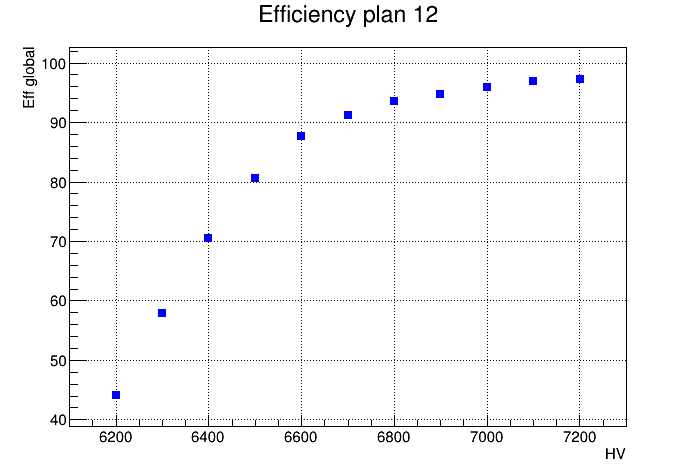
\includegraphics[width=.49\textwidth]{SDHCAL/figs/plateau12.png}
    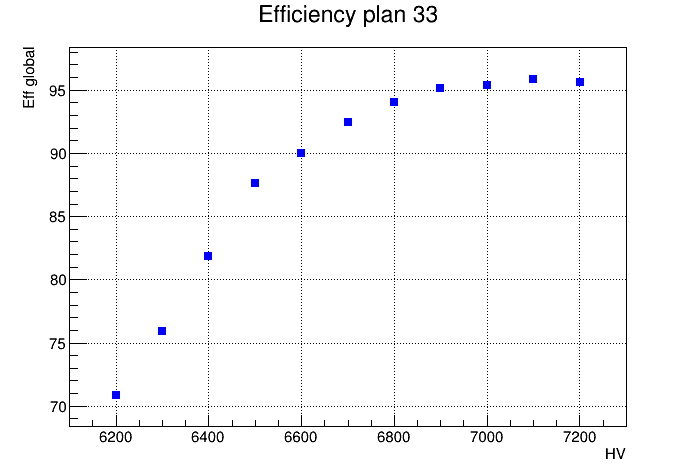
\includegraphics[width=.49\textwidth]{SDHCAL/figs/plateau33.png}
    \caption{Courbes d'efficacité (en $\%$) de deux GRPC en fonction de la haute tension appliquée (en $V$). Le plateau d'efficacité est atteint autour de 6.8 $kV$.}
    \label{fig:plateau}
  \end{center}
\end{figure}
La tension choisie doit se situer sur le plateau. Ainsi, des variations des conditions extérieures (température, pression) auront peu d'impact sur les efficacités des détecteurs. Pour les tests en faisceau de 2012, la haute tension appliquée sur les détecteurs était de 6.9 $kV$. Lors des tests de 2015, nous avons refait les courbes d'efficacité en fonction de la tension et nous avons réglé les tensions pour que tous les détecteurs soient au même endroit sur le plateau. Ces tensions variaient de 6.8 à 7.2 $kV$. De plus, lors de ces tests, les tensions étaient corrigées en fonction de la température extérieure $T$ et de la pression atmosphérique $P$ afin de conserver une amplification constante dans la couche de gaz. La nouvelle tension $V_{i}$, à appliquer sur le détecteur $i$, était calculée selon la formule suivante:
\begin{equation}
  V_{i}=V_{i,ref}\frac{T_{ref}}{P_{ref}}\frac{P}{T}
\end{equation}
où $V_{i,ref}$ est la tension initiale choisie, $T_{ref}$ et $P_{ref}$ sont les valeurs de température et de pression atmosphérique de référence, mesurées lors de l'étude de l'efficacité en fonction de la tension (cf. figure~\ref{fig:plateau}). Cette correction était appliquée lorsque la différence entre la nouvelle valeur de tension et celle de référence dépassait 20 $V$. 
\subsubsection{Seuils utilisés}
Les seuils ont été optimisés avec la simulation pour obtenir une bonne résolution en énergie. Ils ont été fixés à 114 $fC$, 5 $pC$ et 15 $pC$. Cependant, ces réglages ont été effectués avec une simulation grossière. Des études de simulation (cf. chapitre~\ref{chap.simulation}) sont actuellement en cours pour ré-optimiser ces valeurs. La méthode consiste à faire varier les valeurs des seuils 2 et 3 puis de reconstruire l'énergie des gerbes hadroniques. La méthode pour reconstruire l'énergie des gerbes hadroniques sera décrite dans la section~\ref{sec.ereco} de ce chapitre.
\begin{figure}[!ht]
  \begin{center}
    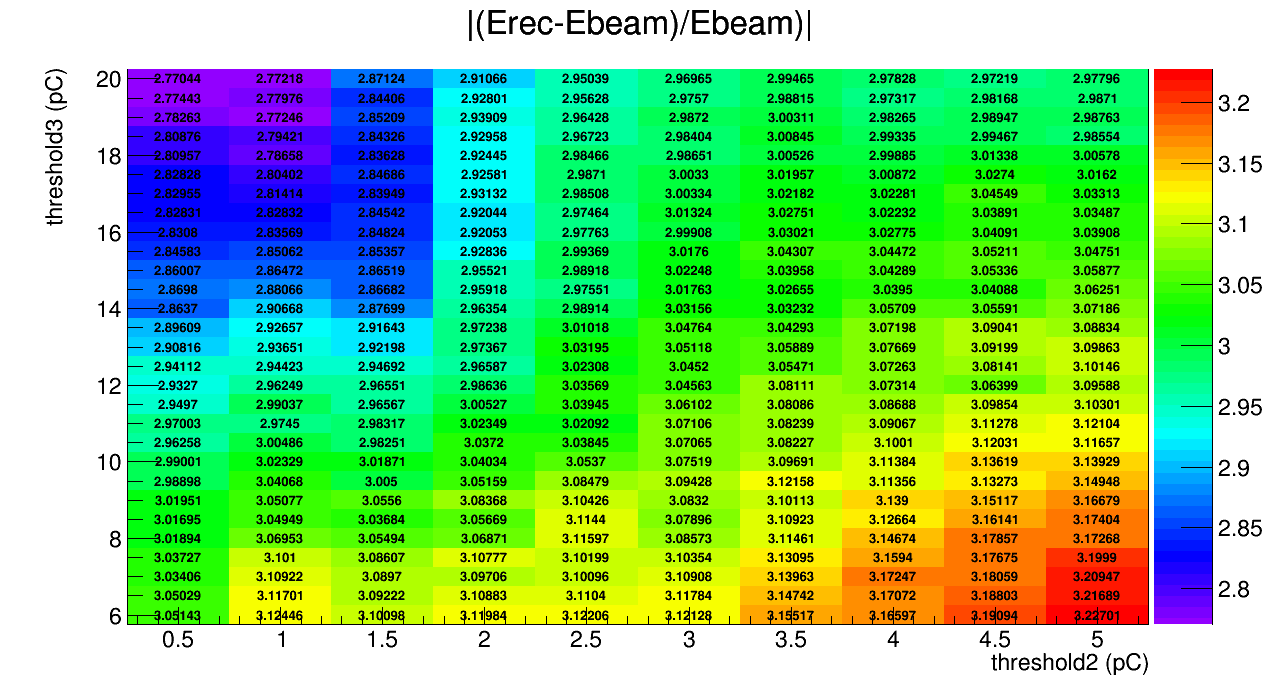
\includegraphics[width=1.\textwidth]{SDHCAL/figs/cumulLinear.png}
    \caption{Déviation relative moyenne (en $\%$) en fonction de la valeur du deuxième et du troisième seuils.}
    \label{fig:lin_vs_thr}
  \end{center}
\end{figure}
\begin{figure}[!ht]
  \begin{center}
    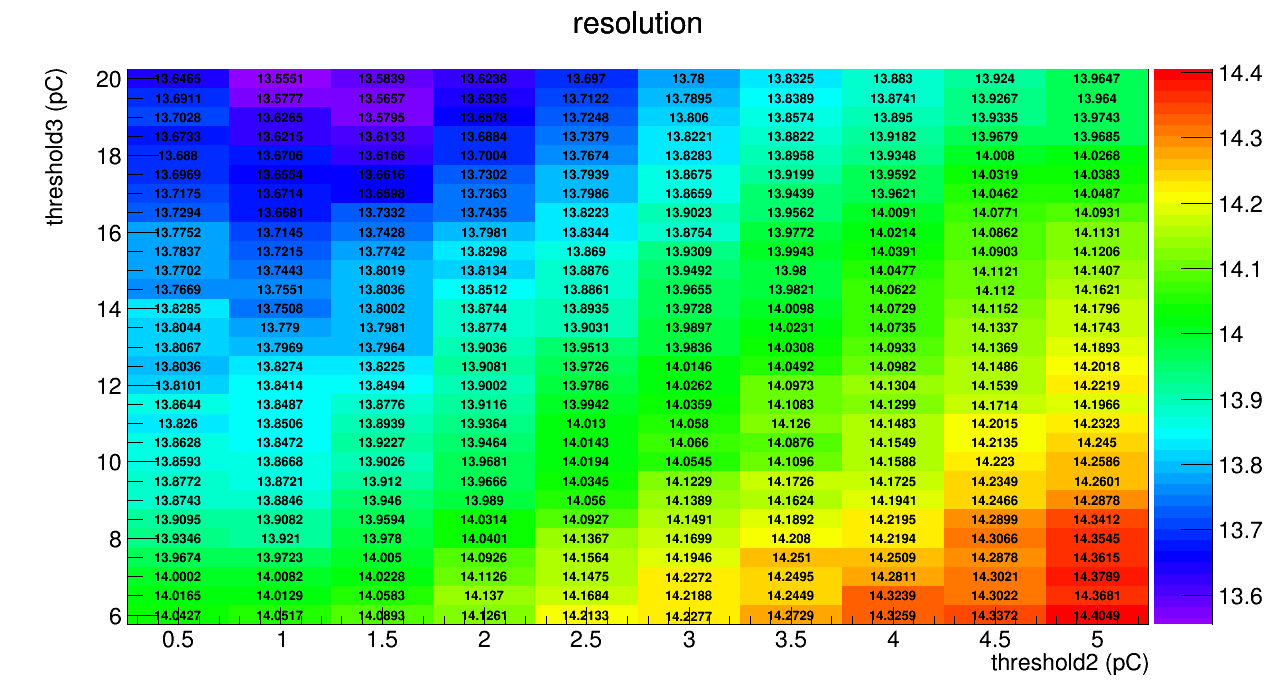
\includegraphics[width=1.\textwidth]{SDHCAL/figs/cumulResol.png}
    \caption{Résolution relative moyenne (en $\%$) en fonction de la valeur du deuxième et du troisième seuils.}
    \label{fig:res_vs_thr}
  \end{center}
\end{figure}
La figure~\ref{fig:lin_vs_thr} montre la déviation relative moyenne définie par $\big<\frac{|E_{reco}-E_{beam}|}{E_{beam}}\big>$ en fonction de la valeur des seuils 2 et 3, où $E_{reco}$ est l'énergie reconstruite et $E_{beam}$ est l'énergie du faisceau. La figure~\ref{fig:res_vs_thr} montre la résolution relative moyenne en fonction de la valeur des seuil 2 et 3. La résolution correspond à la grandeur $\sigma_{reco}/E_{reco}$, où est $\sigma_{reco}$ l'écart type d'une distribution gaussienne obtenue en ajustant les distributions de l'énergie reconstruite. On constate que la déviation relative diminue et la résolution s'améliore pour des faibles valeurs du seuil 2 et des valeurs élevées du seuils 3. Ces résultats préliminaires indiquent que de régler les seuils 2 et 3 vers 1 et 15 $pC$ permettraient d'améliorer légèrement les performances du détecteur. Il n'est malheureusement pas possible d'augmenter la valeur du troisième seuil avec la version actuelle de l'ASIC HARDROC. Avec la nouvelle génération d'ASIC HARDROC, il sera possible d'aller jusqu'à 10 et 50 $pC$ pour respectivement les seuils 2 et 3. 

\subsection{Correction des gains}
\label{sec.gainCorrect}
Tous les canaux des ASIC possèdent un préamplificateur de charge. Ils sont utilisés pour augmenter ou diminuer le signal d'un canal avant l'entrée du signal dans les discriminateurs. Le signal peut être multiplié par un gain allant de 0 à 2. Lors des tests en faisceau de 2012, tous les gains du prototype étaient réglés à 1. Lors des tests en faisceau de 2015, nous avons mis en œuvre une méthode de correction des gains pour réduire le bruit dans le détecteur et surtout pour améliorer l'homogénéité de la réponse des GRPC. Cette méthode est basée sur une analyse du bruit dans le prototype. Nous avons utilisé des données sans faisceau. Pour ne pas biaiser l'analyse, les événements physiques (cf. section~\ref{sec.trivent}) sont rejetés. En effet, même sans faisceau il reste les particules cosmiques dans les échantillons de données. De plus, les bruits cohérents dus à des problèmes de masse sont aussi filtrés: les coups d'horloge (1 coup = 200 $ns$) avec plus de 50 signaux dépassant le premier seuil sont rejetés. Il suffit alors de compter le nombre de hits enregistrés dans chaque canal pendant la prise de données. La figure~\ref{fig:noise_and_gain}(a) montre la distribution du nombre de hits de bruits de chaque canal lors d'une prise de donnée.
\begin{figure}[!ht]
  \subfigure[]{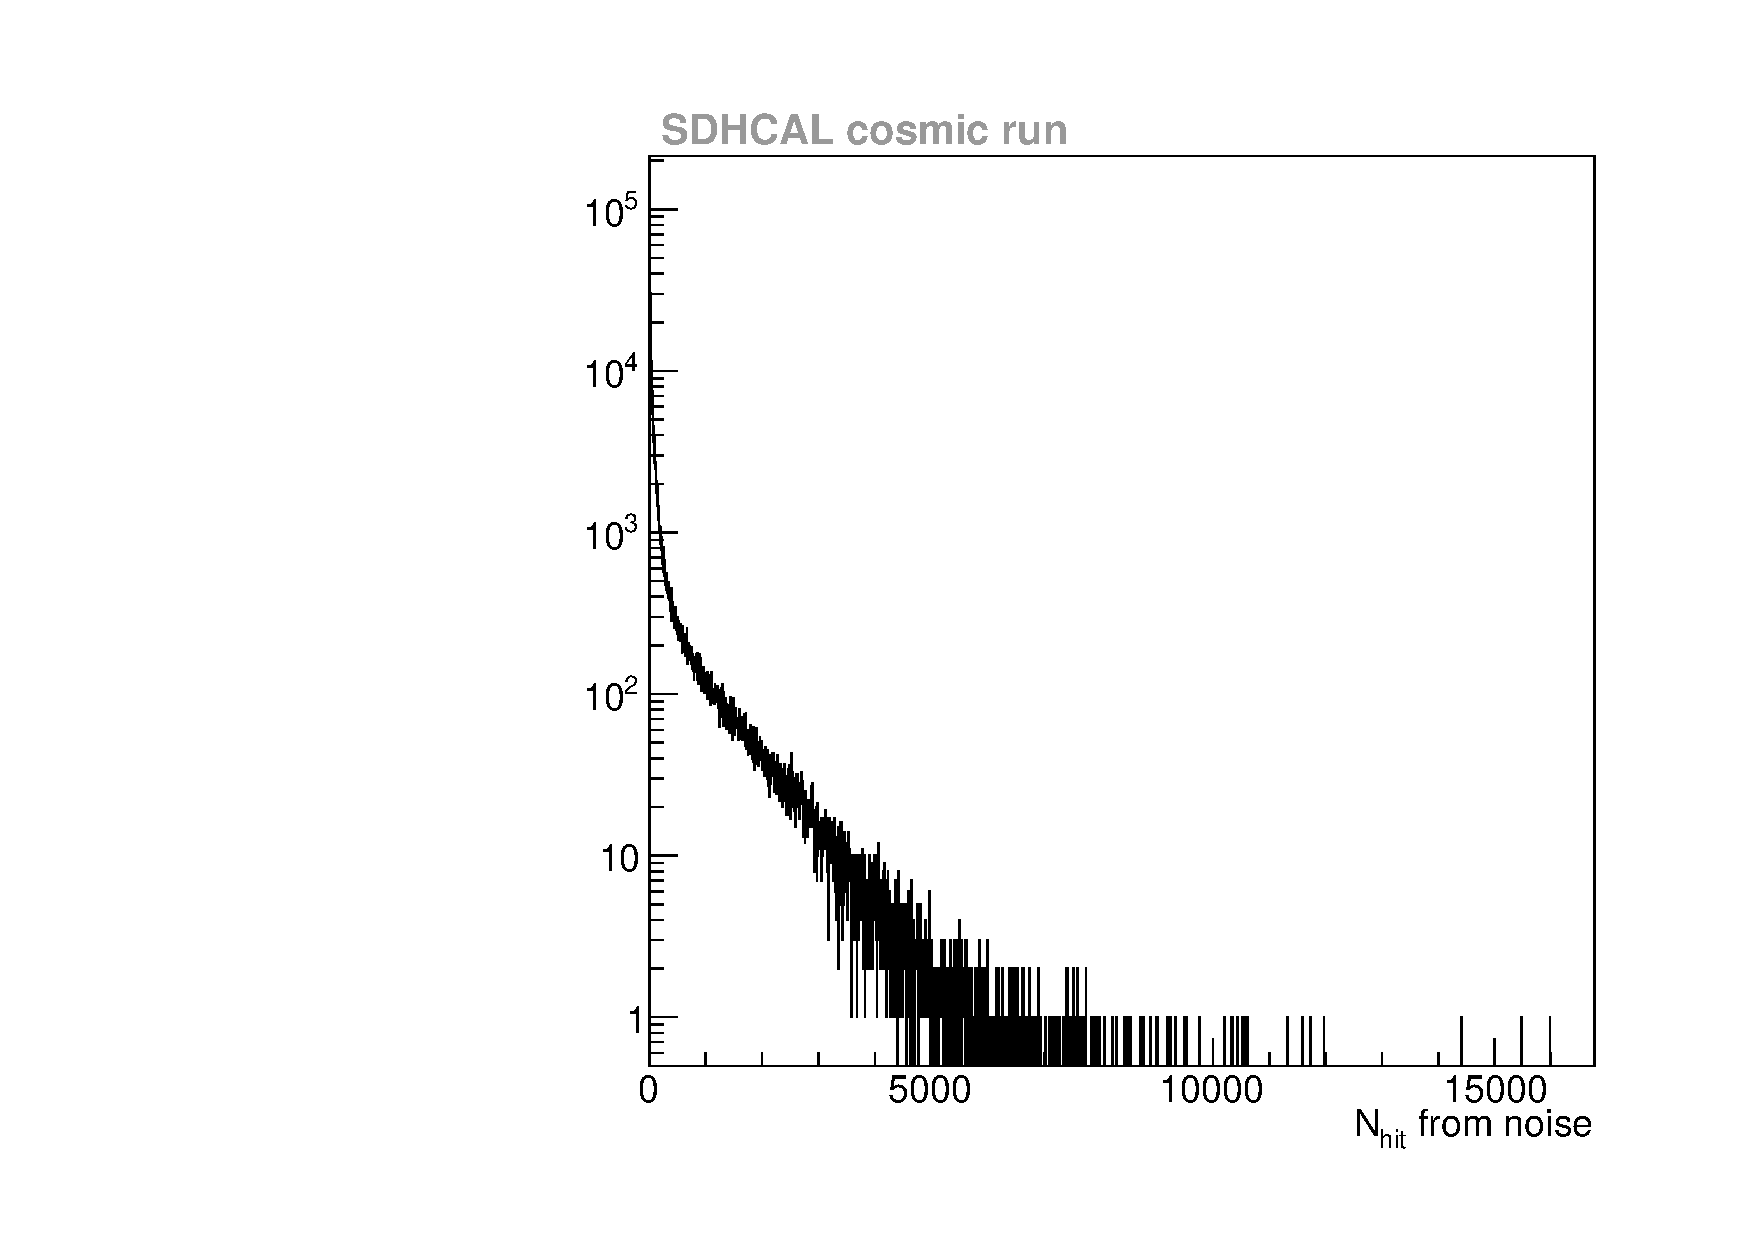
\includegraphics[width=.5\textwidth]{SDHCAL/figs/noise.pdf}}
  \subfigure[]{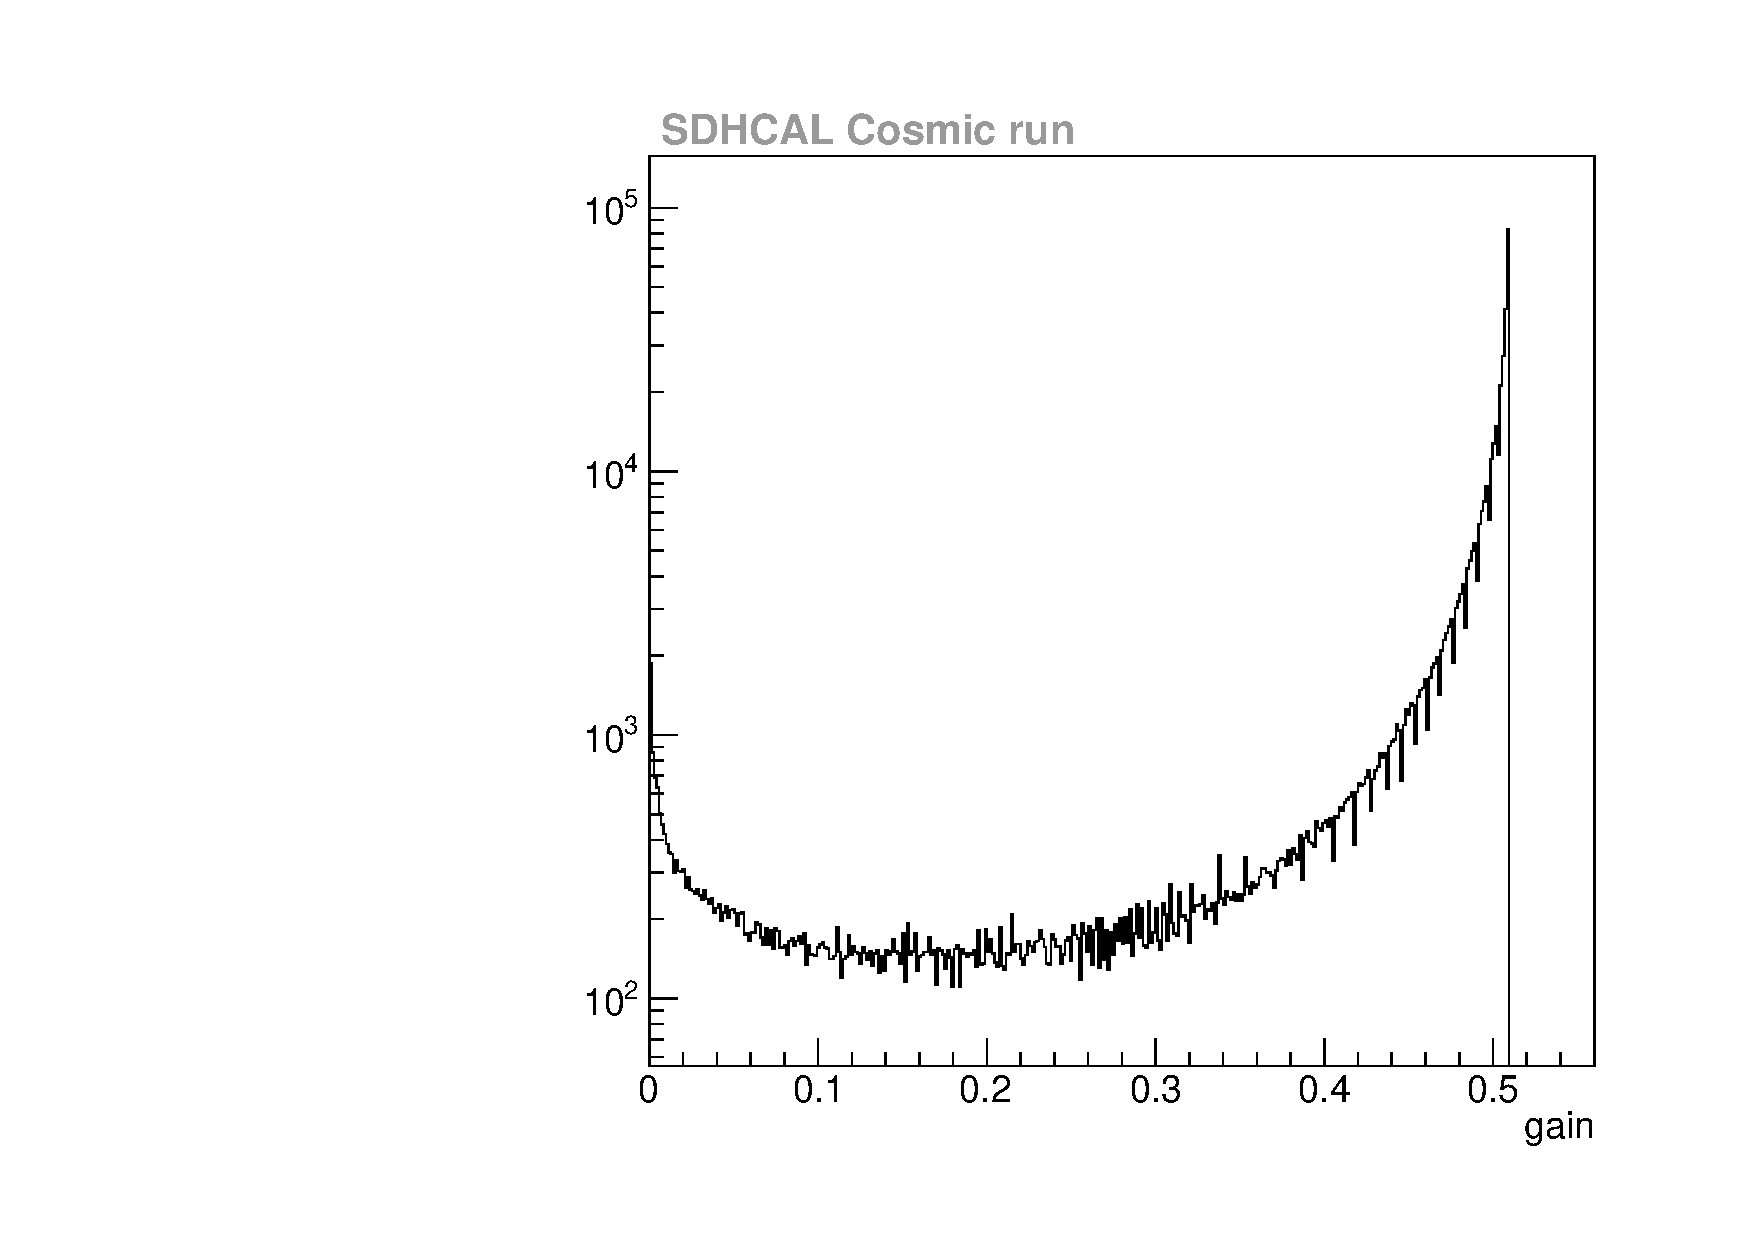
\includegraphics[width=.5\textwidth]{SDHCAL/figs/gain.pdf}}
  \caption{Distribution du nombre de hits de bruits pour chaque canal lors d'une prise de donnée sans faisceau(a). Distribution des gains (non normalisé) calculés à partir de l'équation~\ref{eq.new_gain} (b).\label{fig:noise_and_gain}}
\end{figure}
Les valeurs des nouveaux gains sont calculées pour chaque canal à l'aide de la fonction suivante:
\begin{equation}
  g_i=\frac{1}{1+e^{\frac{N_i-\tilde{N}}{\sigma_N}}}
  \label{eq.new_gain}
\end{equation}
où $N_i$ correspond au nombre de hits de bruits dans le canal $i$, $\tilde N$ et $\sigma_N$ sont la valeur médiane et l'écart type de la distribution du bruit (figure~\ref{fig:noise_and_gain}(a)). La figure~\ref{fig:noise_and_gain}(b) montre la distribution des nouveaux gains. Cette distribution est alors normalisée pour avoir un gain moyen égal à 1 sur tout le détecteur. Ces nouveaux gains, permettent de masquer les canaux les plus bruyants et ainsi de prendre des données dans de meilleures conditions. 
\begin{figure}[!ht]
  \subfigure[]{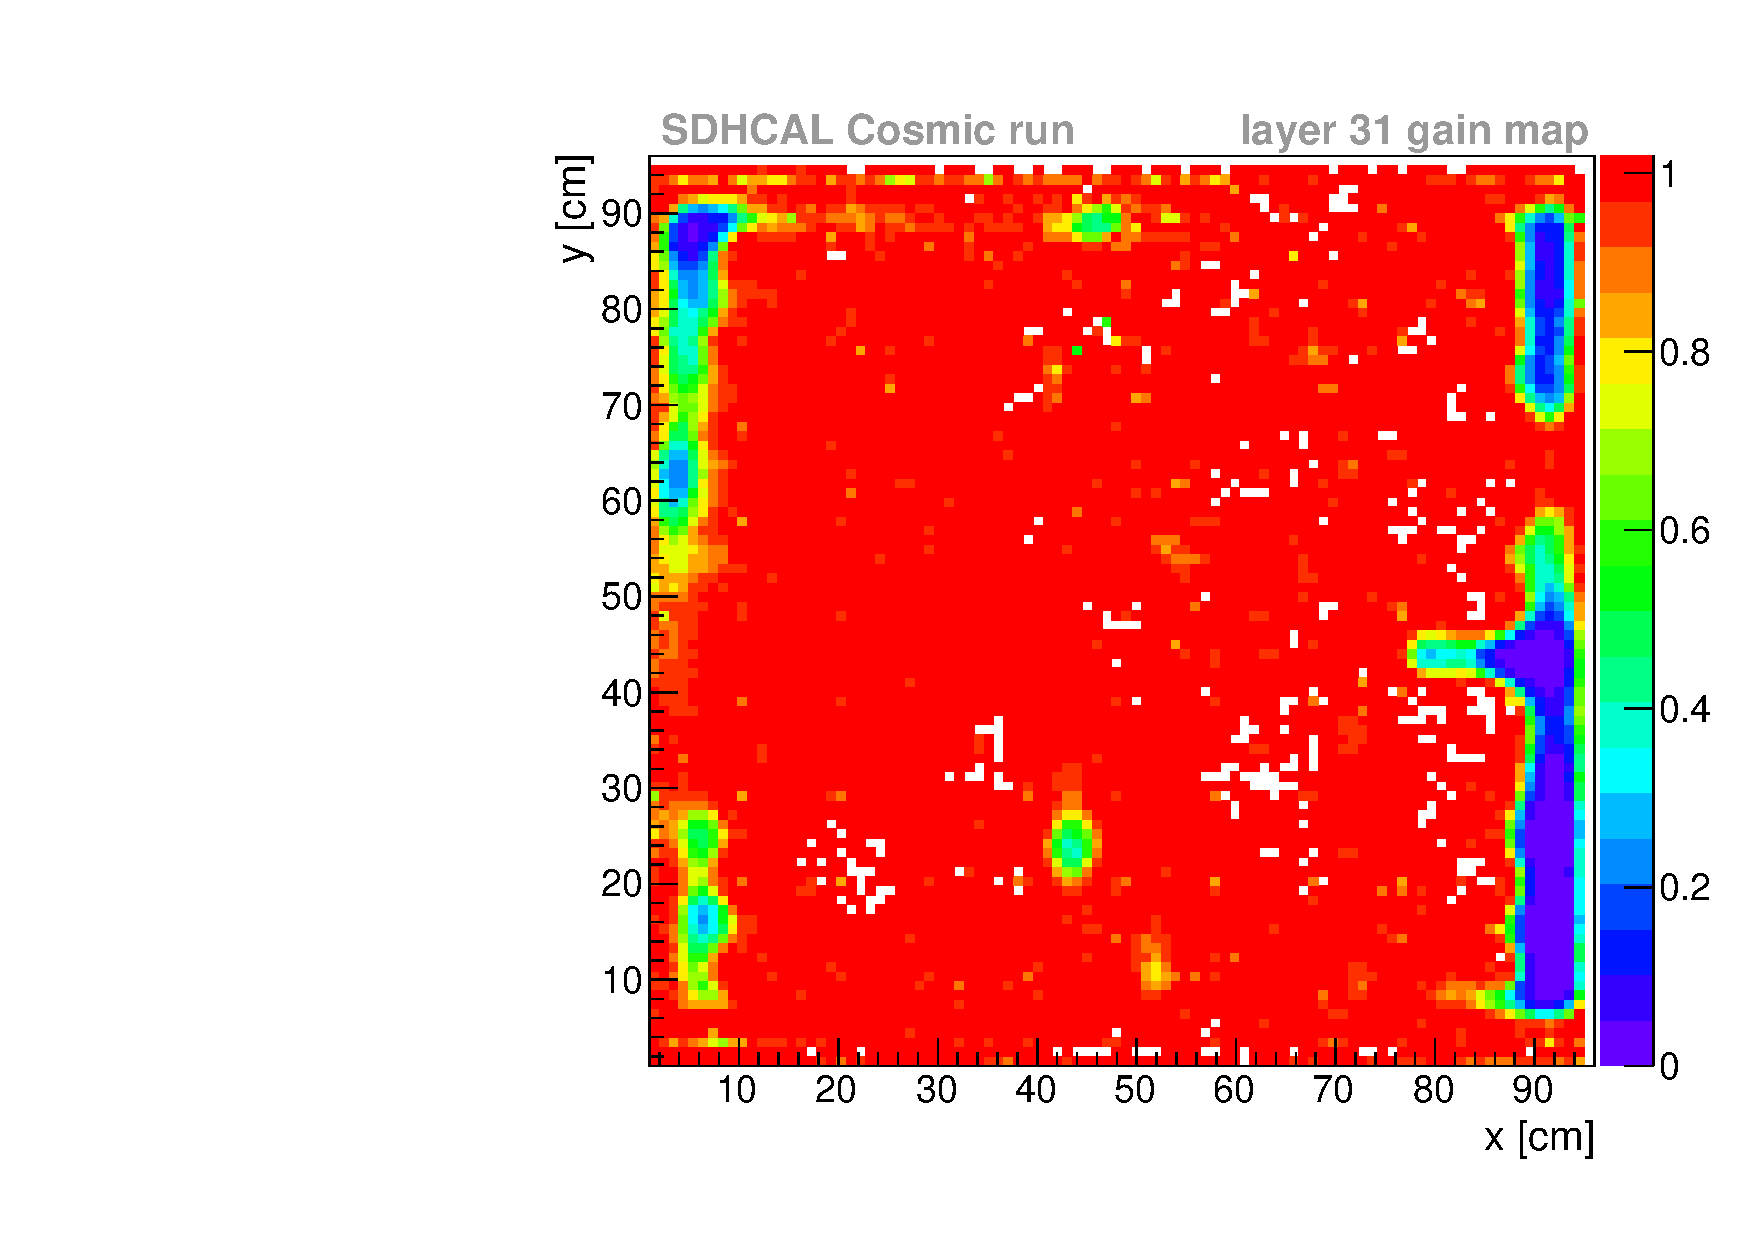
\includegraphics[width=.5\textwidth]{SDHCAL/figs/gainMap31.pdf}}
  \subfigure[]{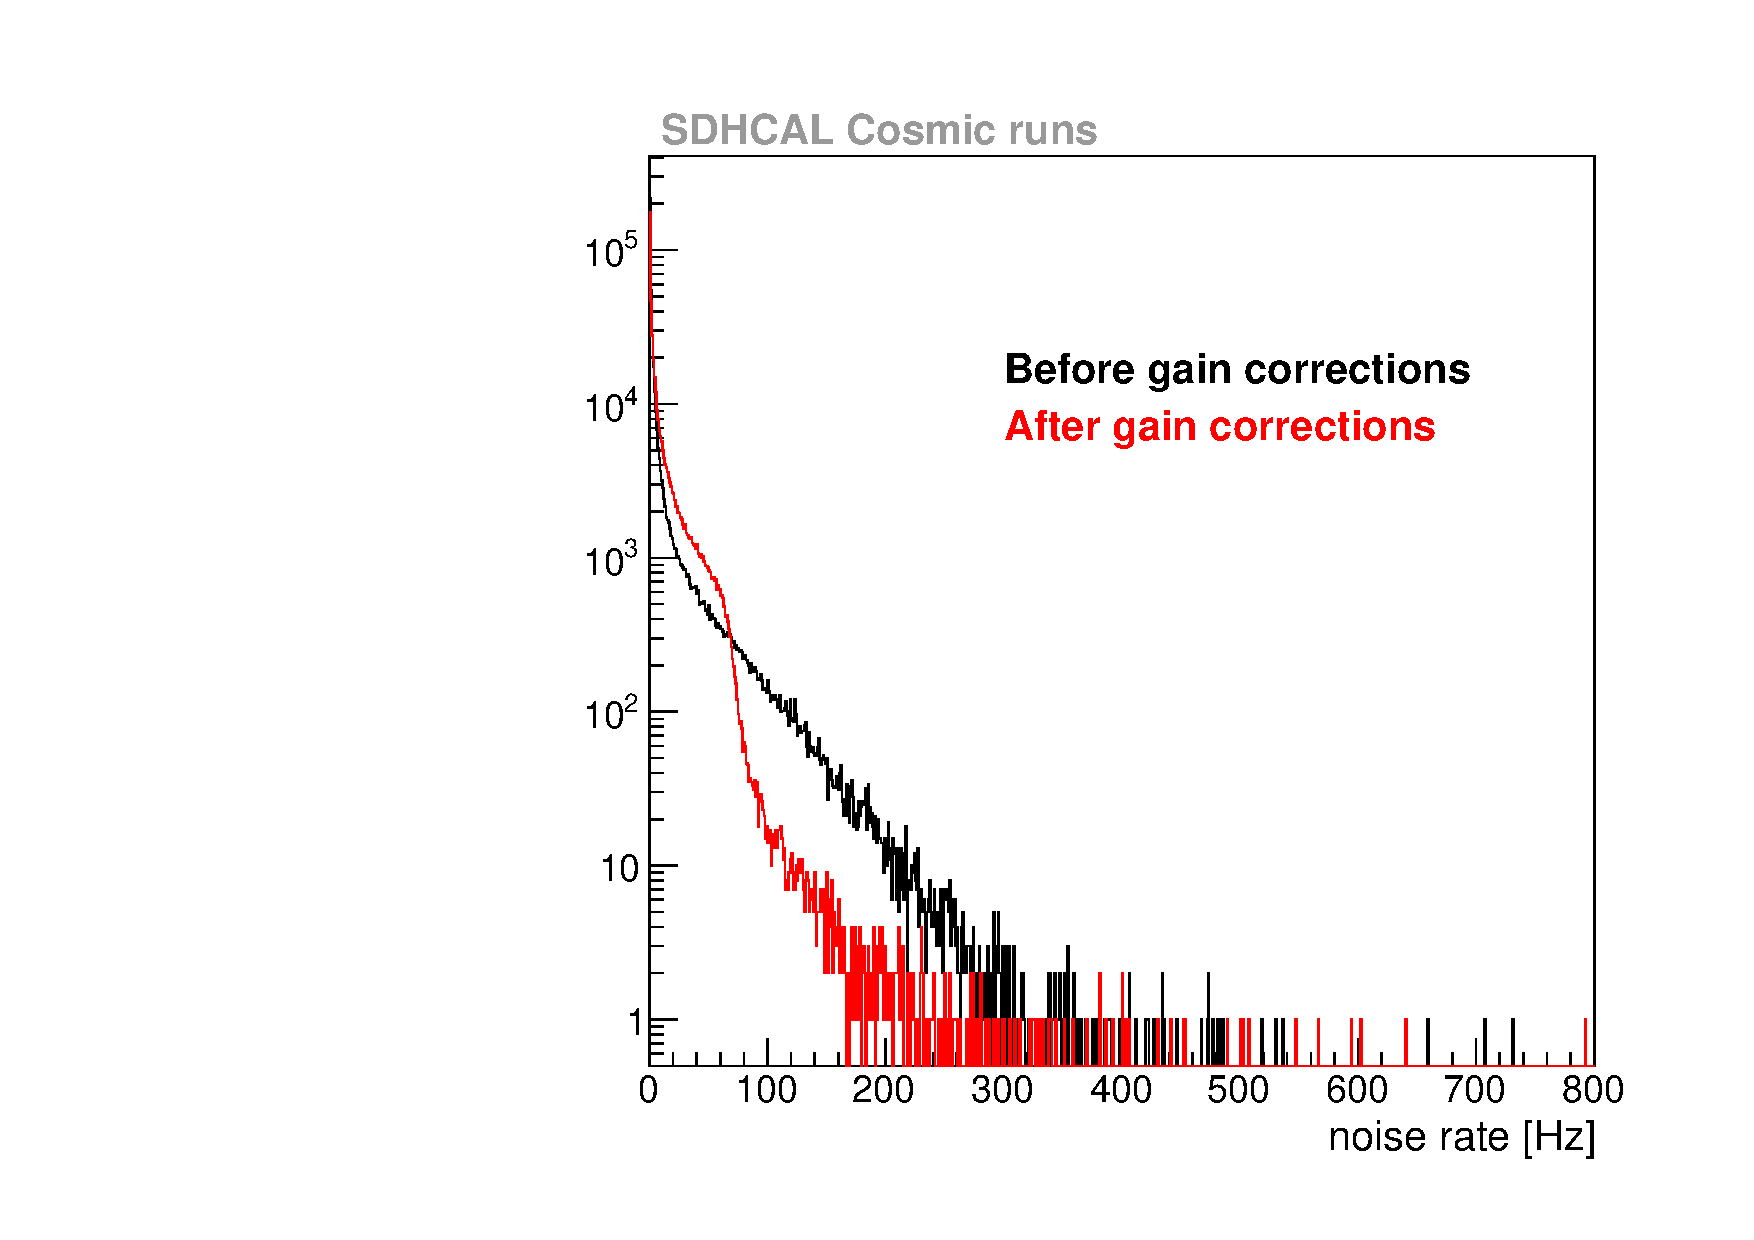
\includegraphics[width=.5\textwidth]{SDHCAL/figs/noiseRate.pdf}}
  \caption{Carte des gains de la chambre 31 du prototype SDHCAL (a). Distribution du taux de bruit dans chaque canal avant (en noire) et après (en rouge) les corrections de gain (b).\label{fig:map_and_rate}}
\end{figure}
La figure~\ref{fig:map_and_rate}(a) montre un exemple de carte de gains pour une chambre du prototype. Les zones en bleu correspondent aux zones les plus bruyantes et sont presque masquées après la correction. Les zones blanches sont, soit des zones non bruyantes, soit des zones déjà masquées. Le gain maximal est appliqué aux canaux non bruyants. La figure~\ref{fig:map_and_rate}(b) montre la distribution du taux de bruit pour chaque canal avant et après la correction de gains. Après la correction des gains, le nombre de canaux ayant un taux de bruits supérieur à 100 $Hz$ diminue sensiblement. Ceci a pour effet d'améliorer nos conditions de prises de données. En effet, le temps d'acquisition qui correspond au temps entre le début d'un cycle d'acquisition et le signal RAMfull augmente sensiblement après les corrections de gain (43 $ms$ après corrections contre 22 $ms$ avant). 

Les analyses préliminaires des données avec les corrections de gain n'ont montré ni d'amélioration, ni de détérioration significative pour la mesure de l'énergie des gerbes hadroniques. Cette méthode de correction, basée sur le bruit dans le détecteur, permet d'améliorer les conditions de prises de données. D'autres méthodes de correction pourront être développées pour améliorer l'homogénéïté de la réponse du détecteur. Dans la suite de ce manuscrit, les résultats sont obtenus avec des données collectées sans correction des gains.

%%%%%%%%%%%%%%%%%%%%%%%%%%%%%%%%%%%%%%%%%%%%%%%

\section{Reconstruction de l'énergie dans le SDHCAL}
Nous avons décrit le prototype du SDHCAL et particulièrement les GRPC qui composent sa partie active. Plusieurs campagnes de prise de données sur les lignes de faisceau H2 et H6 au CERN ont été réalisées. Dans la suite de cette section, les différentes méthodes développées pour reconstruire l'énergie des hadrons incidents sont décrites. 
\subsection{Reconstruction des événements}
\label{sec.trivent}
Nous avons déjà mentionné que le mode de lecture du prototype utilisé en test sur faisceau rend obligatoire une procédure de reconstruction des événements. Dans les données collectées, on trouve les événements physiques (muons du faisceau et cosmiques, gerbes hadroniques et électromagnétiques) et du bruit. Pour séparer les événements physiques du bruit, nous utilisons une méthode de groupement temporel des hits \cite{sdhcal-com}. Pour chaque événement RAMfull, les hits sont classés en fonction de leur temps d’occurrence. Rappelons que ce temps est échantillonné par pas de 200 $ns$ grâce à l'horloge interne des ASIC. La figure~\ref{fig:time_spectrum} montre un exemple de la distribution du temps des hits dans un événement RAMfull. 
\begin{figure}[!ht]
  \begin{center}
    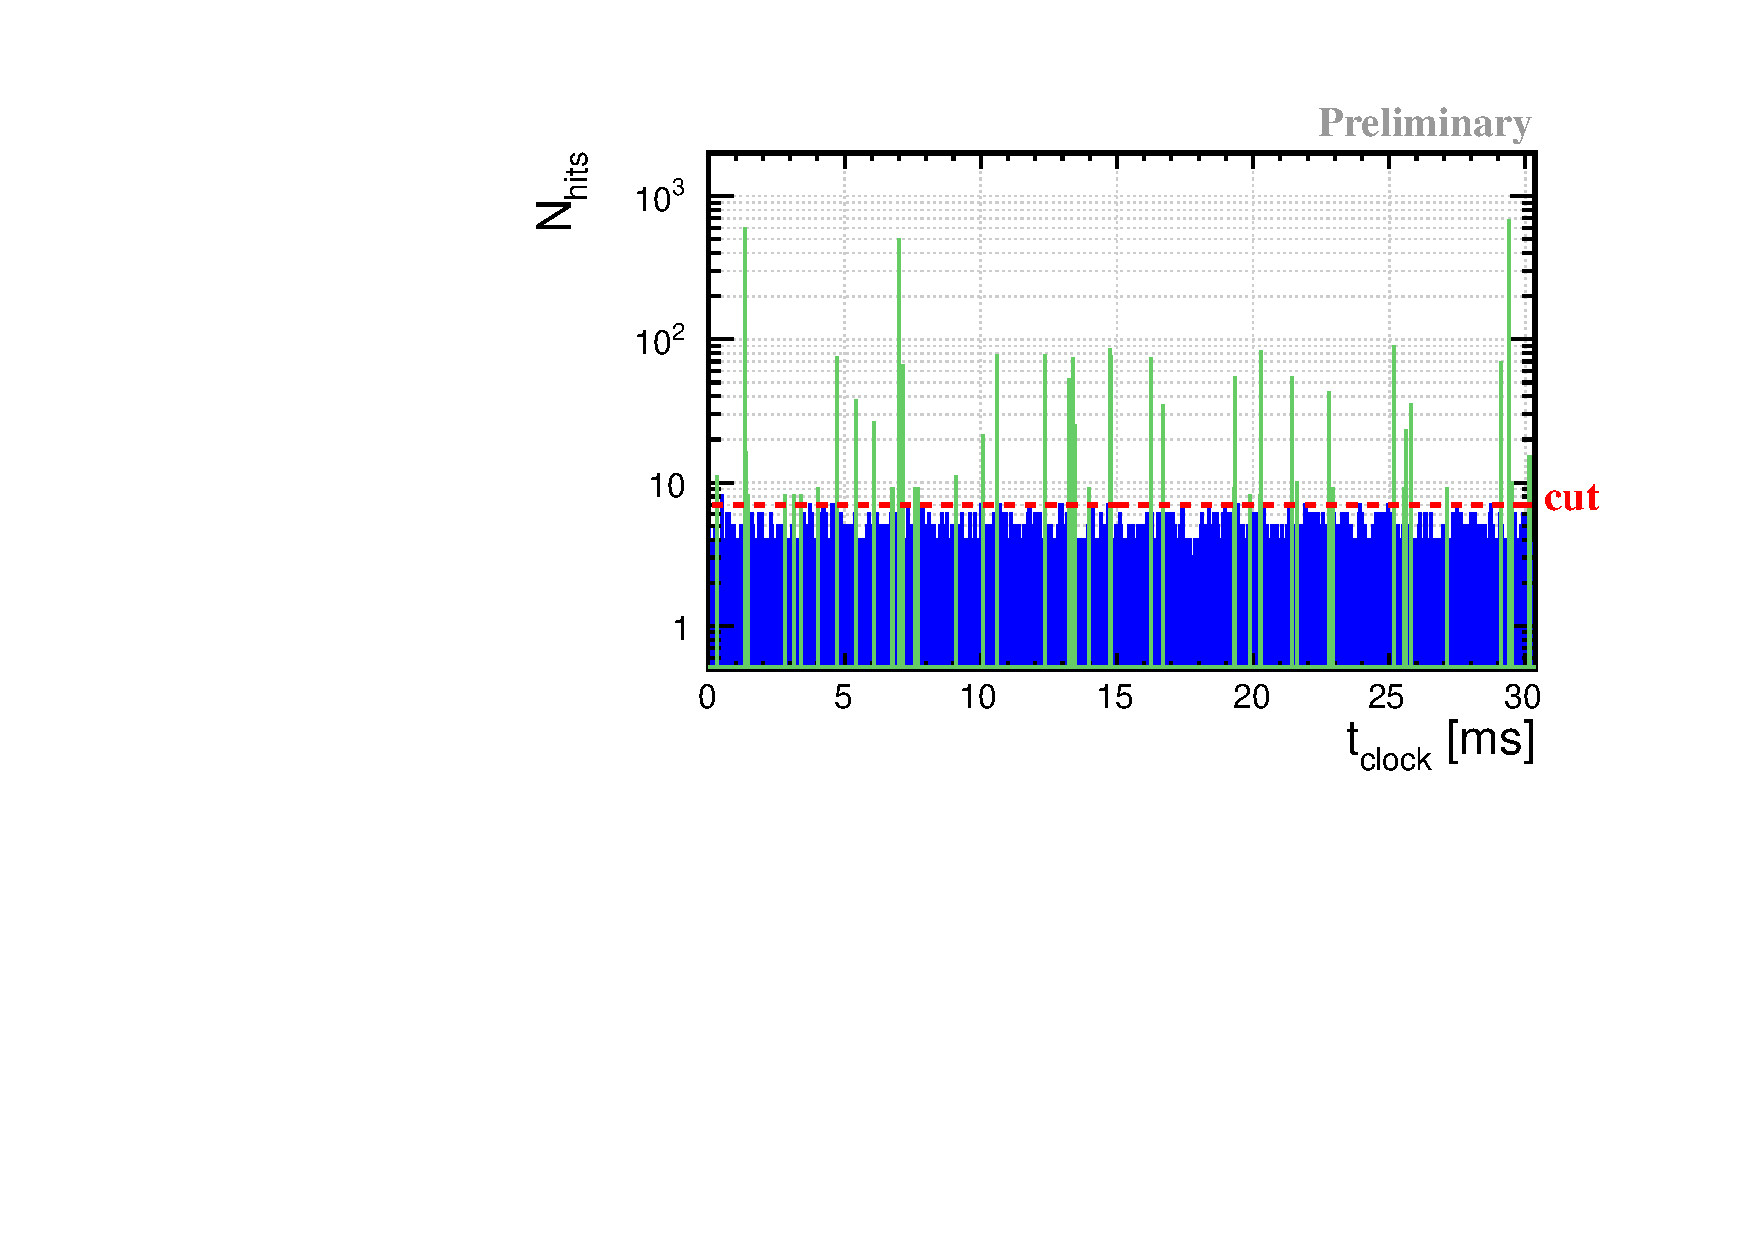
\includegraphics[width=.9\textwidth]{SDHCAL/figs/time_spectrum.pdf}
    \caption{Distribution du temps des hits dans un événement RAMfull. Les bins en vert correspondent aux fenêtres en temps qui sont utilisées comme candidats d'événements physiques.}
    \label{fig:time_spectrum}
  \end{center}
\end{figure}
Lorsque dans un créneau d'horloge $t_0$ (1 créneau=200 $ns$), le nombre de hits est suffisant (>7 sur la figure~\ref{fig:time_spectrum}), un candidat d'événement physique est créé. Ce candidat est conservé seulement s'il correspond à un maximum local ($\Delta_t=600~ns$) de la distribution de la figure~\ref{fig:time_spectrum}. Les hits dans les créneaux adjacents ($t=t_0\pm200~ns$) sont ajoutés au candidat. Cependant, il a été observé que certaines DIF pouvaient se désynchroniser des autres d'un coup d'horloge. Pour un faible nombre d'événements, un certain nombre de hits n'apparaissaient pas dans l'événement et les gerbes hadroniques reconstruites semblaient "trouées". Ainsi, la fenêtre de temps pour construire les événements physiques a dû être augmentée ($t=t_0\pm 2\times200~ns$). Un événement physique est finalement reconstruit si le nombre de plans de GRPC avec au moins un hit est supérieur à un paramètre donné ($N_{plans}>=5$ par défaut). Le format des événements physiques est légèrement différent des événement RAMfull. Il contient le temps du RAMfull, le temps relatif au début de leur cycle d'acquisition, les coordonnées des positions de touts les hits de l'événement physique et leur seuil associé. Les hits dans les fenêtres de temps, rejetées par cette procédure sont utilisés pour estimer le bruit du détecteur. 
\begin{figure}[!ht]
  \begin{center}
    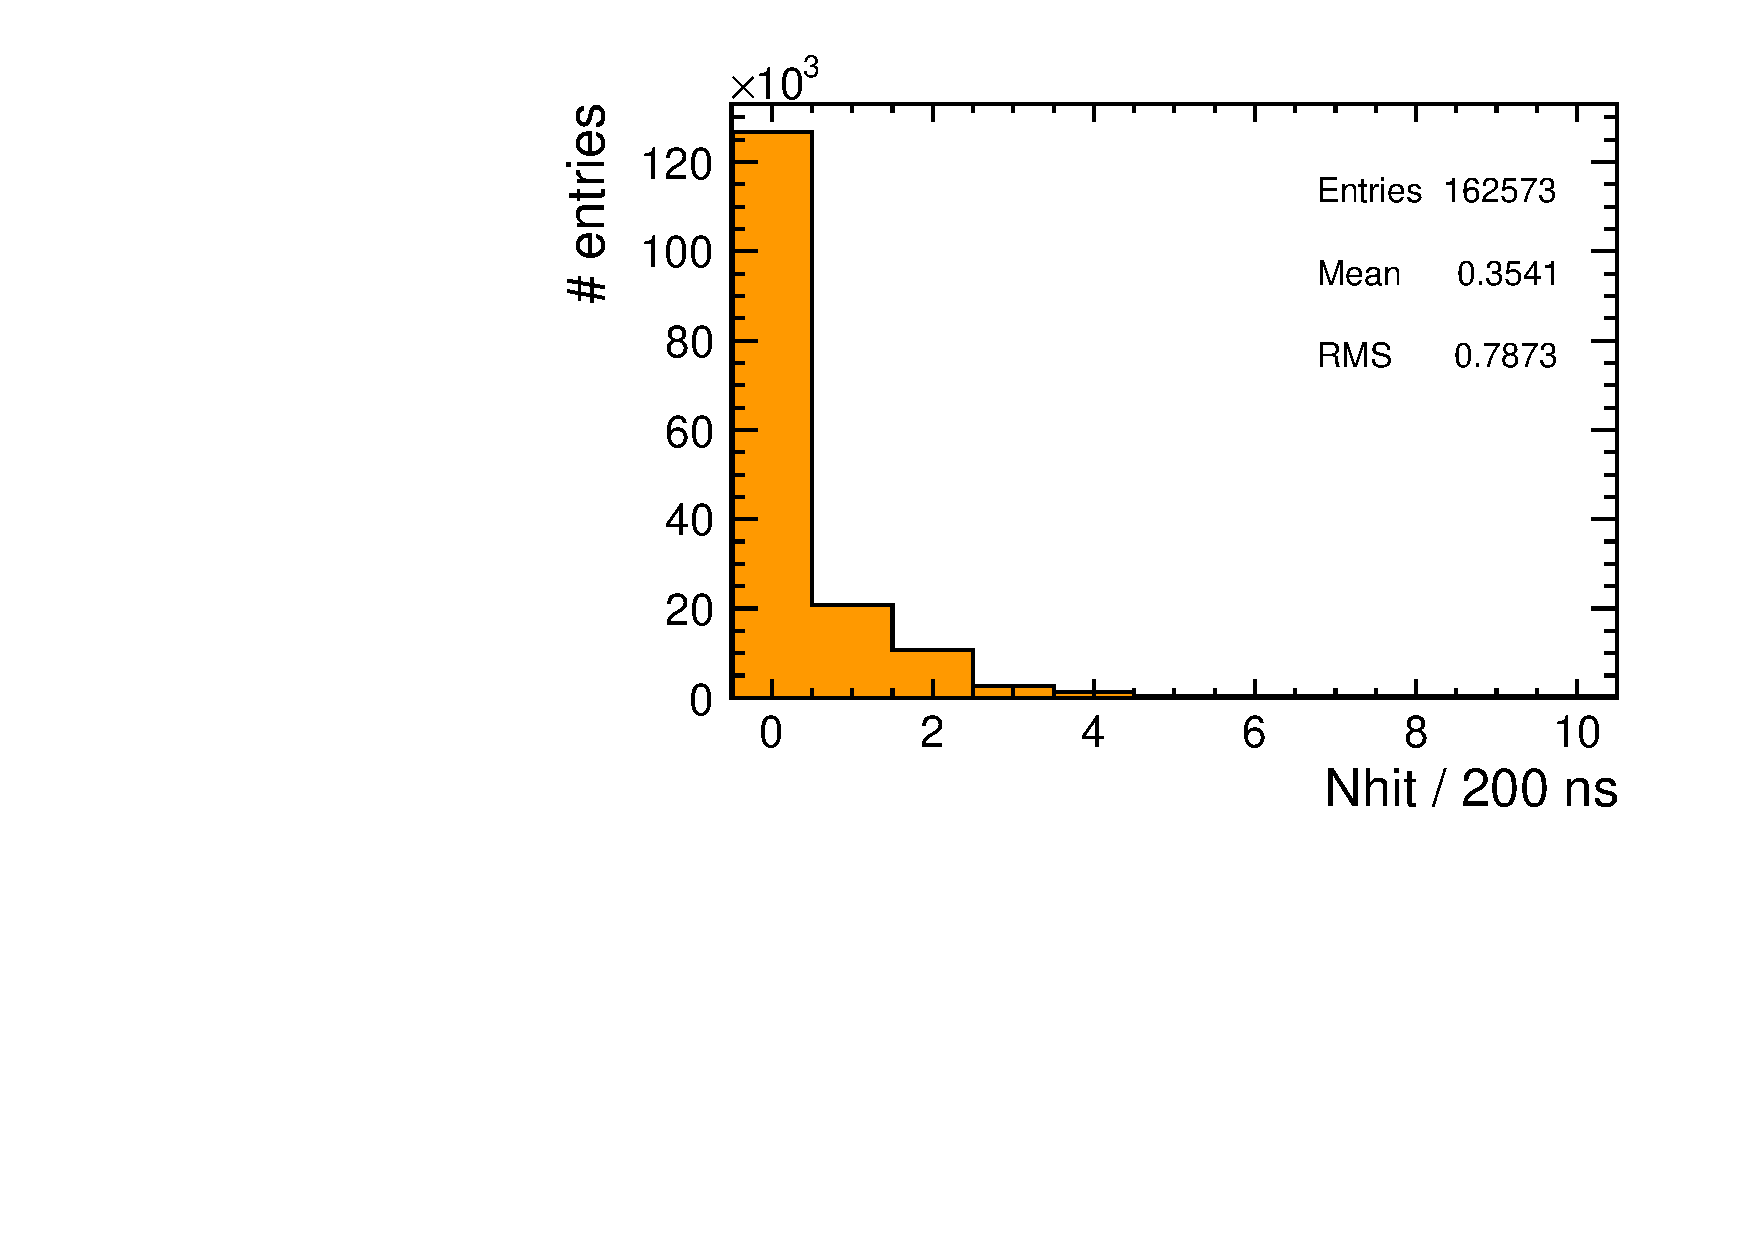
\includegraphics[width=.9\textwidth]{SDHCAL/figs/time_hit_sprectrum_all_centered_R715651_T28.pdf}
    \caption{Distribution du nombre de cellules touchées par du bruit dans un crénau d'horloge. Ces hits correspondent à ceux rejetés par la procédure de reconstruction des événements physiques.}
    \label{fig:noise_spectrum}
  \end{center}
\end{figure}
La figure~\ref{fig:noise_spectrum} montre la distribution du nombre de hits de bruit dans un créneau d'horloge pour le prototype SDHCAL. La valeur moyenne de cette distribution ($\approx 0.35~hits/200ns$) nous permet d'estimer le bruit moyen à 1.75 hits par événement physique reconstruit. 
\subsection{Performance du SDHCAL}
\label{sec.muons}
Pour étudier les performances du prototype, l'efficacité et la multiplicité sont deux variables très importantes. L'efficacité correspond à la présence d'un signal détecté lors du passage d'une particule et la multiplicité correspond au nombre de canaux déclenchés lorsqu'une seule particule (MIP) traverse la couche de gaz. Ces deux variables correspondent aux propriétés intrinsèques des GRPC. L'efficacité et la multiplicité sont étudiées pour de nombreuses applications. Les programmes de surveillance (monitorage) utilisés en test sur faisceau, calculent ces variables, ce qui permet rapidement de vérifier la qualité de la prise de données. Nous verrons dans le chapitre~\ref{chap.simulation} qu'une mesure précise de ces propriétés est indispensable pour la simulation du détecteur.
\subsubsection{Reconstruction des traces}
Pour étudier ces deux variables, qui représentent la réponse du détecteur au passage d'une seule particule, nous utilisons les événements muons. Ces événements sont reconstruits avec la procédure décrite dans la section~\ref{sec.trivent} de ce chapitre. Cependant, lors des tests en faisceau, nous n'avons pas pu utiliser de compteur Cerenkov pour identifier la nature des particules. Il est donc nécessaire d'utiliser une procédure de sélection des événements muons et ainsi de rejeter les gerbes hadroniques et électromagnétiques présentes dans nos échantillons de données. Une analyse en composante principale PCA (Principal Component Analysis) permet efficacement de sélectionner des candidats de traces. Une PCA consiste à diagonaliser la matrice de covariance. Cette matrice est une matrice $3\times3$ et ses éléments $M_{i,j}$ sont calculés avec l'équation suivante:
\begin{equation}
  M_{i,j}=\sum_{k=0}^{N_{hits}}{(q_{i,k}-\bar{q_i})(q_{j,k}-\bar{q_j})}
\end{equation}
où les $q_{i,k}$ sont les coordonnées des positions des hits et les $\bar q_i$ sont les coordonnées du barycentre des hits de l'événement. Ces éléments sont ensuite normalisés avec la trace de cette matrice. Les valeurs propres $\lambda_i$ issues de la diagonalisation de la matrice sont classées par ordre décroissant. La valeur propre $\lambda_1$ est associée au vecteur propre qui donne la direction principale de l'événement. Les valeurs propres $\lambda_2$ et $\lambda_3$ sont associées aux directions transverses. Le rapport $\frac{\sqrt{\lambda_2^2+\lambda_3^2}}{\lambda_1}$ est utilisé pour sélectionner les événements muons. La figure~\ref{fig:transverseRatio} montre ce rapport en fonction du nombre de hits. 
\begin{figure}[!ht]
  \begin{center}
    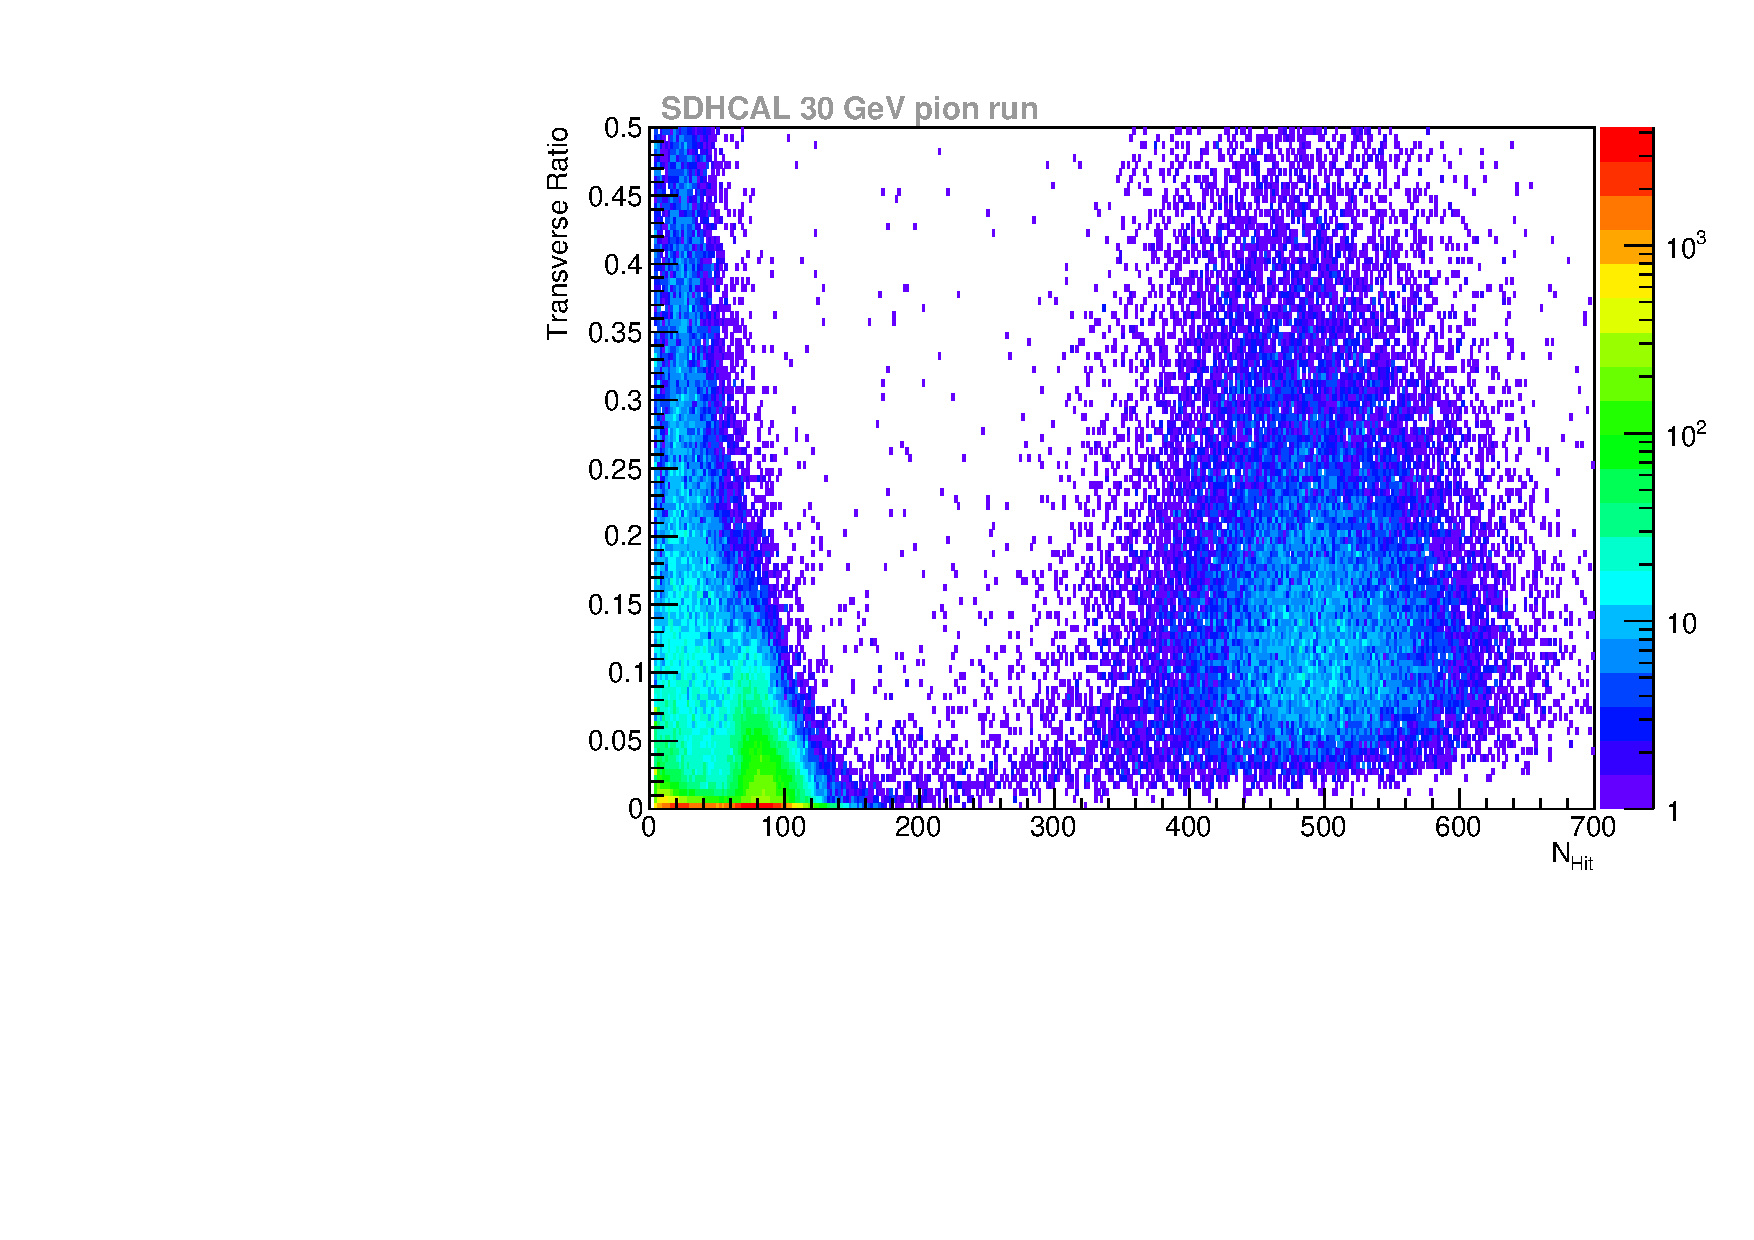
\includegraphics[width=.7\textwidth]{SDHCAL/figs/transverseRatio.pdf}
    \caption{Rapport $\frac{\sqrt{\lambda_2^2+\lambda_3^2}}{\lambda_1}$ (Transverse Ratio) en fonction du nombre de hits ($N_{Hit}$) pour un échantillon de données à 30 $GeV$.}
    \label{fig:transverseRatio}
  \end{center}
\end{figure}
On peut facilement distinguer deux régions sur la figure~\ref{fig:transverseRatio}. La première région pour laquelle le nombre de hits est assez faible ($N_{Hit}<200$) correspond aux muons cosmiques et aux muons du faisceau. La deuxième région ($N_{Hit}>200$) correspond au gerbes hadroniques. Une coupure sur la rapport $\frac{\sqrt{\lambda_2^2+\lambda_3^2}}{\lambda_1}$ à 0.05 permet de conserver une partie importante des muons tout en rejetant la plupart des gerbes hadroniques. Une deuxième procédure de sélection permet d'améliorer la qualité des traces sélectionnées et de rejeter les gerbes hadroniques restantes. Les étapes de cette sélection sont les suivantes:
\begin{enumerate}[-]
\item les hits d'un même plan sont groupés dans des amas lorsqu'ils sont voisins. Les événements dont le nombre d' amas de hits est inférieur à une valeur donnée sont rejetés~($N_{amas}<5$ par défaut). La figure~\ref{fig:amas} présente deux exemples de configurations d'amas possibles;
\begin{figure}[!ht]
  \begin{center}
    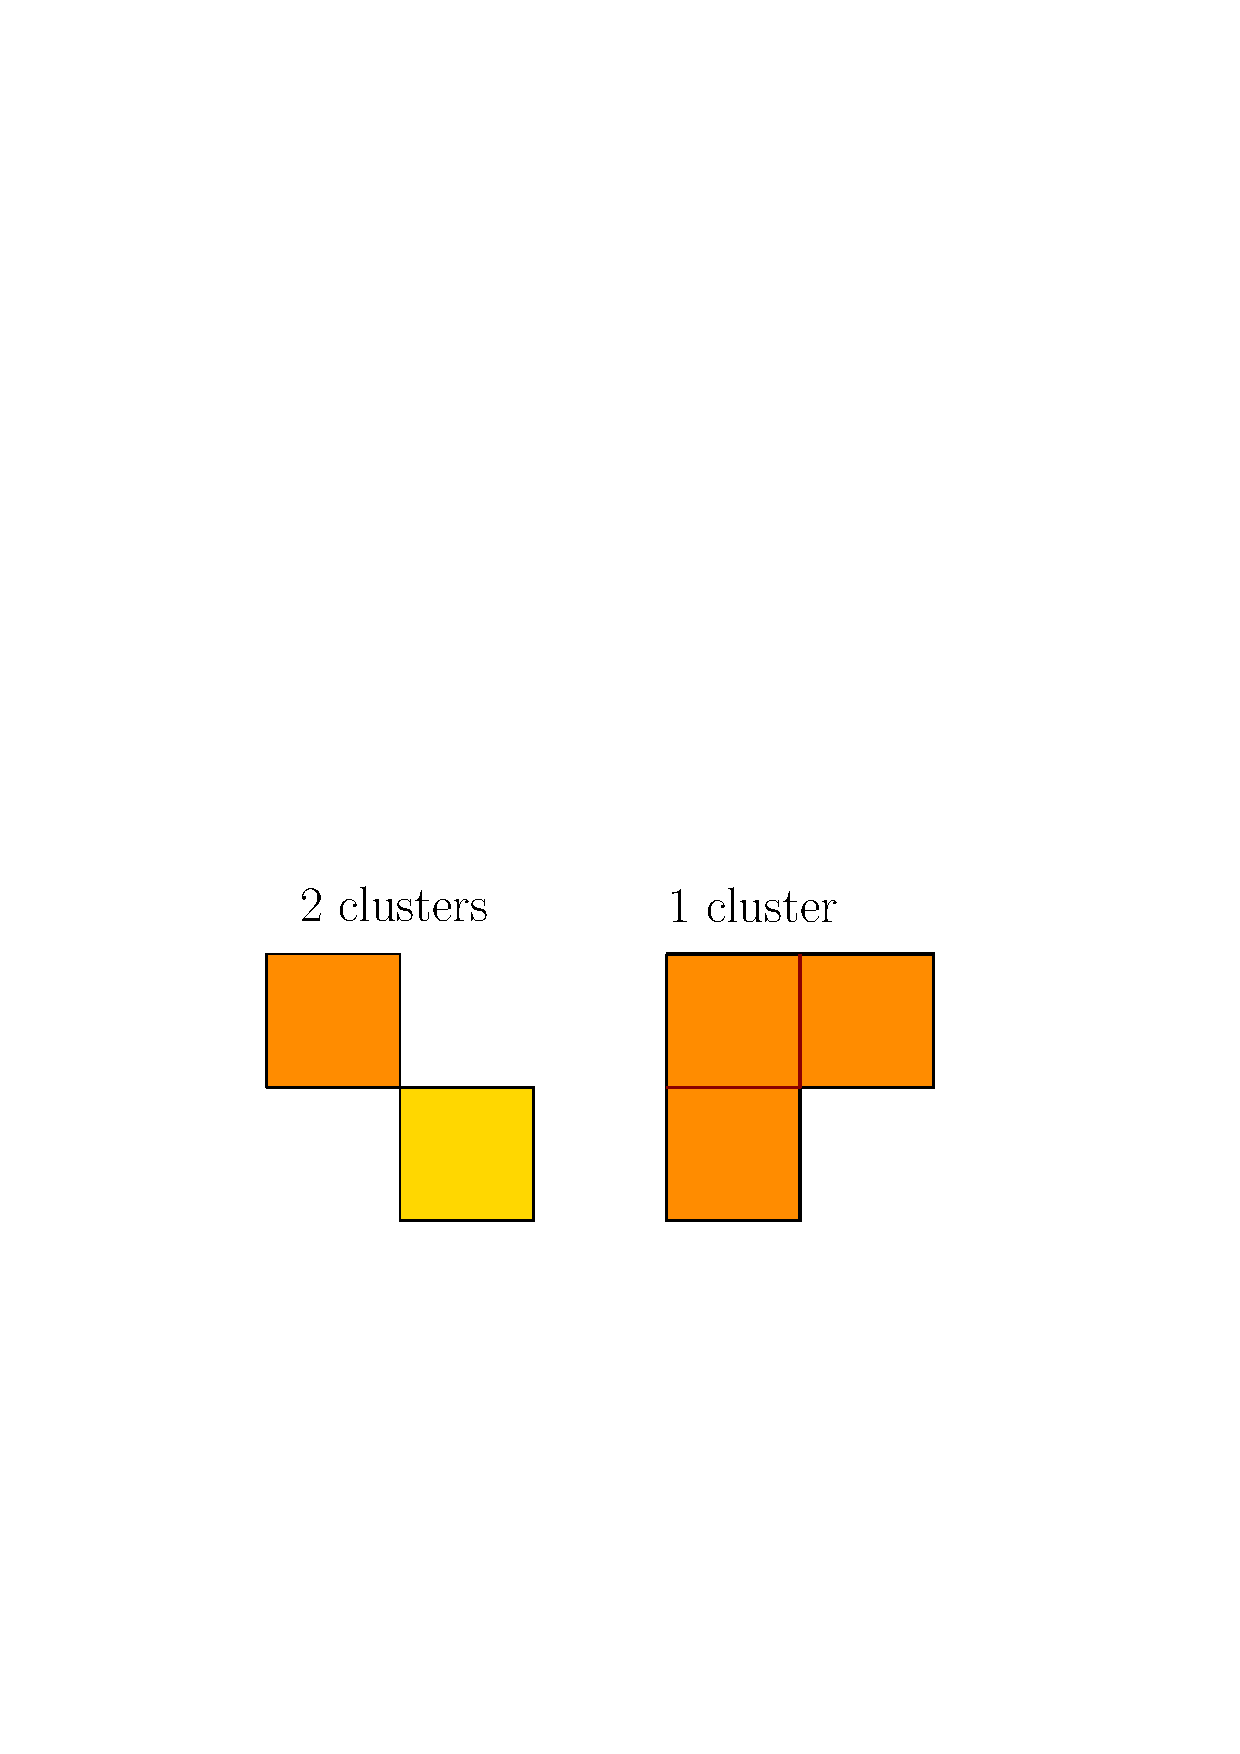
\includegraphics[width=.5\textwidth]{SDHCAL/figs/Clusters.pdf}
    \caption{Exemple de configuration d'amas. A gauche, deux amas sont créés. La configuration de droite conduit à la formation d'un seul amas.}
    \label{fig:amas}
  \end{center}
\end{figure}
\item la trajectoire de la particule est ajustée avec une régression linéaire dans les plans $(xOz)$ et $(yOz)$\footnote{L'axe $(Oz)$ correspond à la direction du faisceau}. Un $\chi^2$ de l'ajustement est calculé  avec l'équation suivante:
  \begin{equation}
    \chi^2=\frac{1}{N_{amas}-1}\sum_{i=0}^{N_{amas}}d_i^2
  \end{equation}
où les $d_i$ correspondent aux distances (en $mm$) entre le barycentre des amas de hits et la droite définie par les coefficients obtenus lors des régressions linéaires. Les événements dont le $\chi^2$ est supérieur à 100 sont rejetés. Ces sélections ont été testées avec des échantillons de simulation de muons dans le SDHCAL. L'efficacité de sélection obtenue avec la simulation est proche de 96$\%$.
\end{enumerate}
\begin{figure}[!ht]
  \begin{center}
    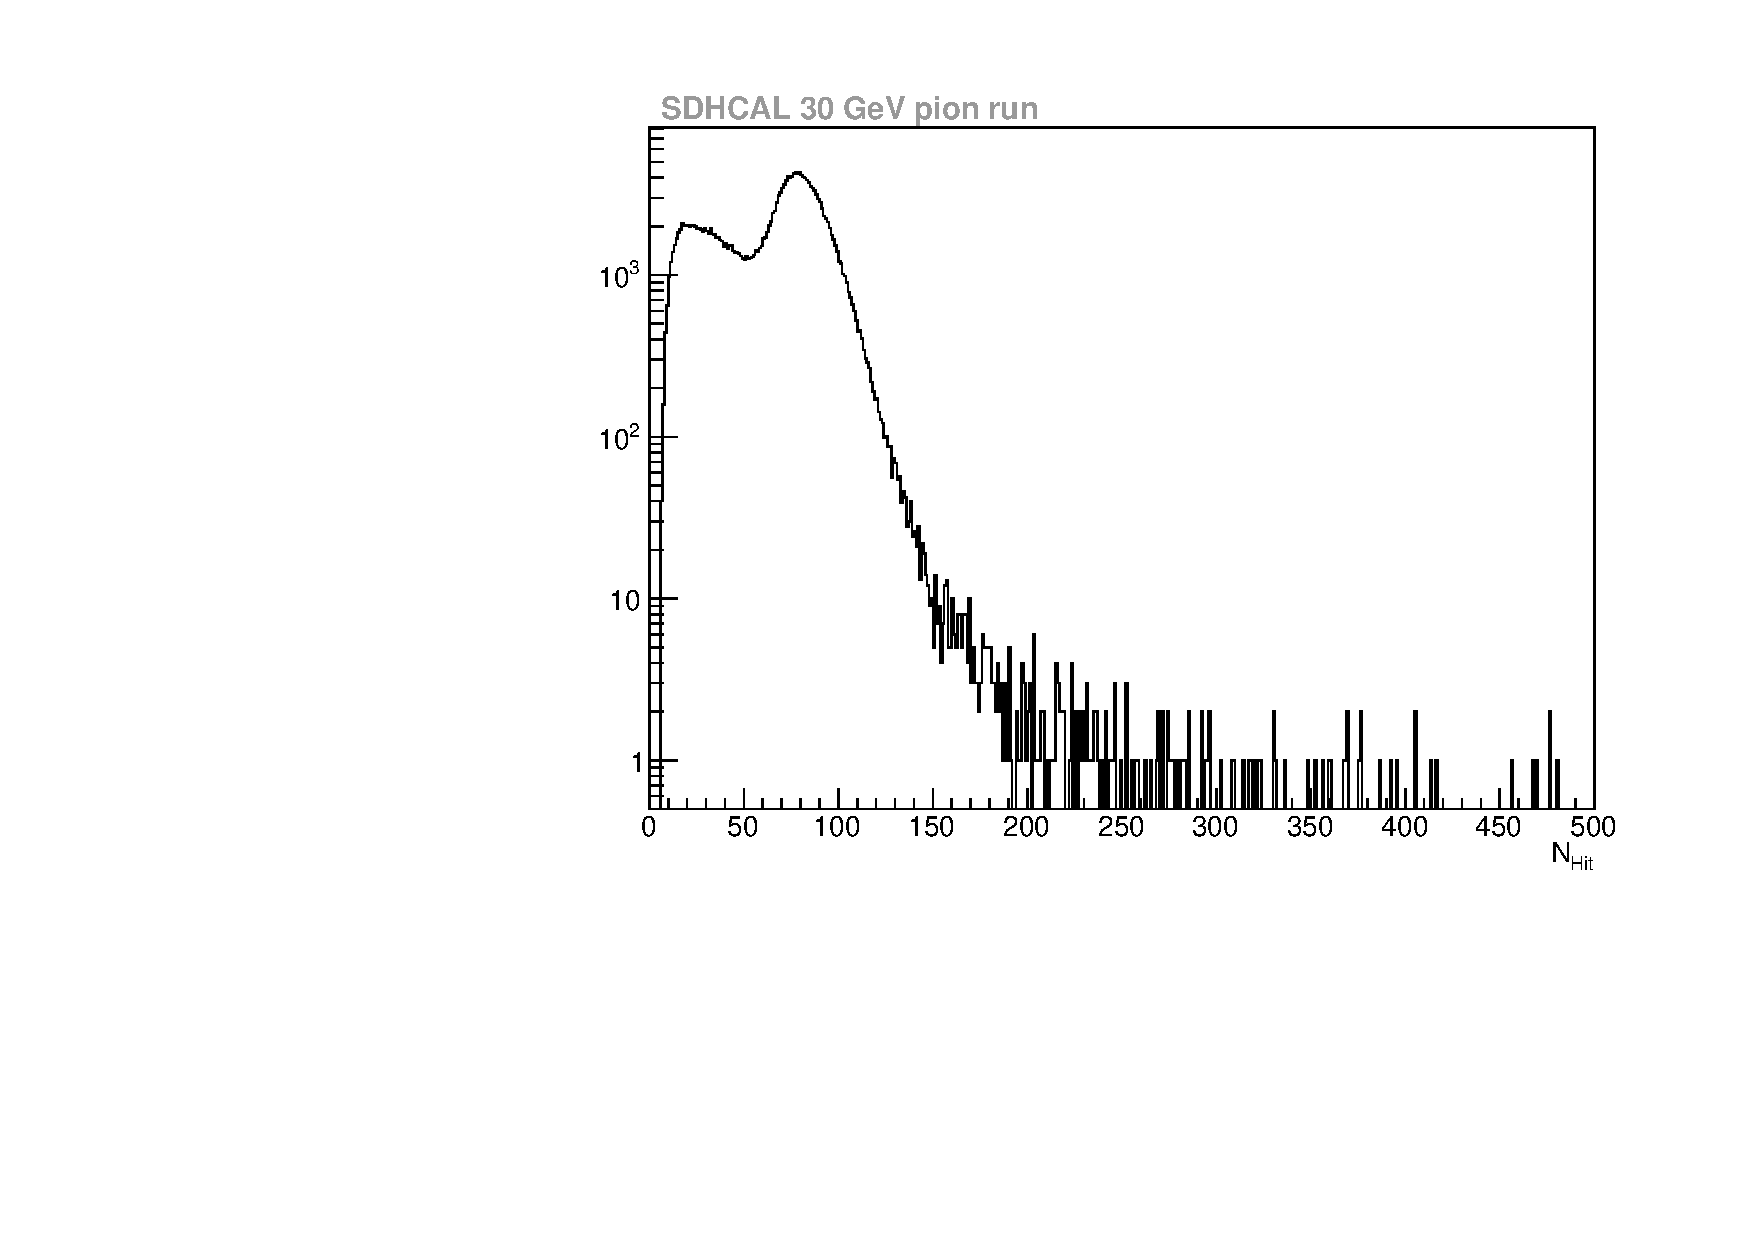
\includegraphics[width=.7\textwidth]{SDHCAL/figs/nhitMuon.pdf}
    \caption{Distribution du nombre de hits ($N_{Hit}$) après sélection des événements muons pour un échantillon de données à 30 GeV.}
    \label{fig:nhitMuon}
  \end{center}
\end{figure}
La figure~\ref{fig:nhitMuon} montre la distribution du nombre de hits ($N_{Hit}$) pour un échantillon de donnée à 30 GeV après les sélections des événements muons. On distingue deux pics sur cette figure. Le premier correspond aux muons cosmiques et le deuxième aux muons du faisceau.
\subsubsection{Efficacité et multiplicité}
Pour chaque muon reconstruit, l'efficacité est estimée pour chaque plan du détecteur susceptible d'être touché par la particule. Pour chacun de ces plans, l'impact de la trace est calculé avec une régression linéaire en utilisant la même méthode que précédemment. Les amas de hits du plan étudié ne sont pas inclus dans la régression linéaire pour éviter tout biais. Un plan est considéré comme efficace si un amas de hits est trouvé à moins de 5 $cm$ de l'impact attendu. La multiplicité correspond alors au nombre de hits dans l'amas correspondant. 
\begin{figure}[!ht]
  \begin{center}
    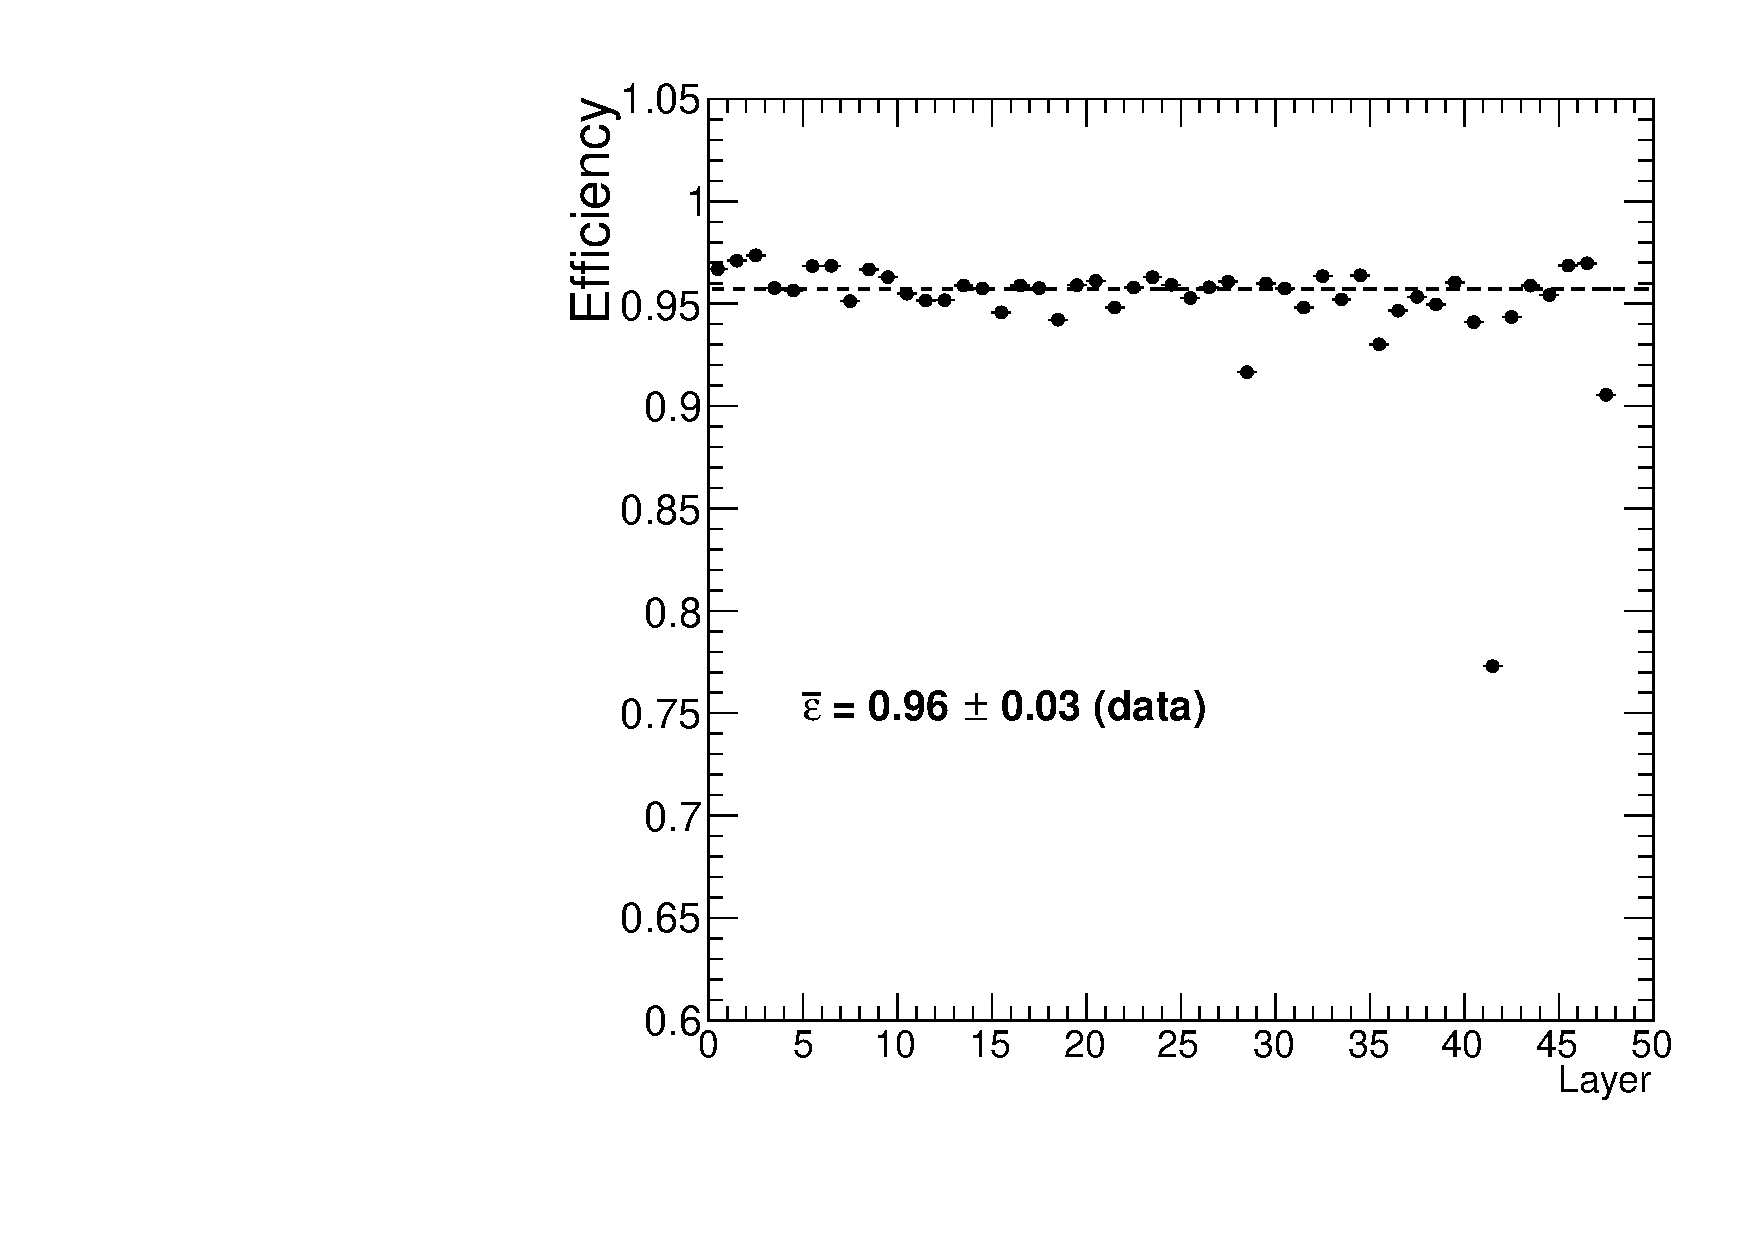
\includegraphics[width=.45\textwidth]{SDHCAL/figs/eff_2012.pdf}
    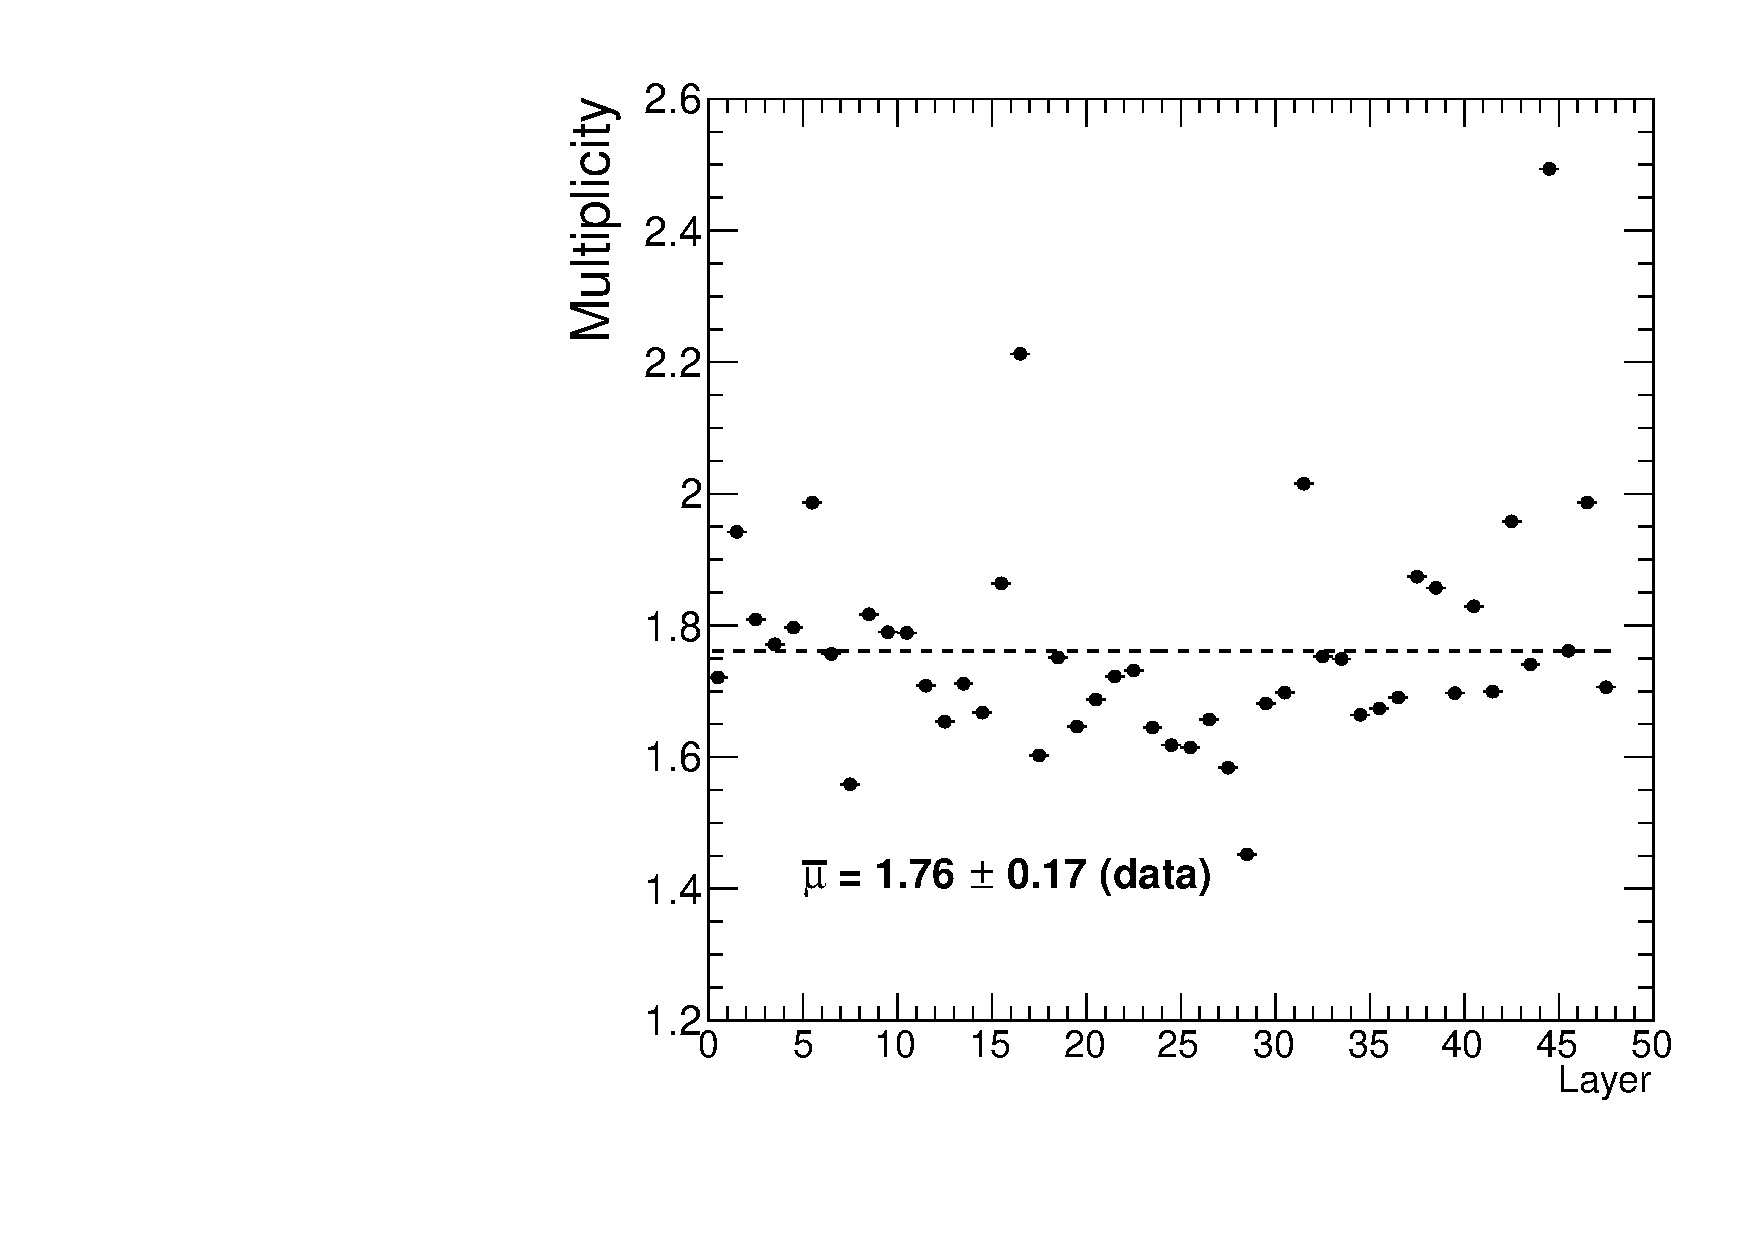
\includegraphics[width=.45\textwidth]{SDHCAL/figs/mul_2012.pdf}
    \caption{Efficacité (à gauche) et multiplicité (à droite) moyenne pour chaque chambre du SDHCAL.}
    \label{fig:eff_and_multi}
  \end{center}
\end{figure}
La figure~\ref{fig:eff_and_multi} montre l'efficacité (à gauche) et la multiplicité (à droite) moyenne pour chaque plan du prototype. L'efficacité moyenne du détecteur est de $96\pm0.03\%$ et la multiplicité moyenne de $1.76\pm0.17$. Les incertitudes sur ces deux valeurs correspond aux écarts types de ces grandeurs. Une partie (environ 1/3) du 42ème plan ne fonctionnait pas, ce qui explique la plus faible efficacité de ce plan ($\varepsilon_{42}\simeq77\%$). La dispersion autour de la multiplicité moyenne est probablement due à des différences de résistivité de la peinture appliquée sur les électrodes d'une chambre à l'autre.
\subsection{Sélection des gerbes hadroniques}
\label{sec.pi_selection}
Nous avons vu la procédure pour sélectionner les événements muons pour calculer l'efficacité et la multiplicité des GRPC. Nous allons maintenant décrire la procédure pour sélectionner les gerbes hadroniques. Rappelons que les échantillons de données contiennent des muons (cosmiques et du faisceau), des gerbes hadroniques et électromagnétiques. Cette procédure de sélection est optimisée pour filtrer les événements muons et les gerbes électromagnétiques, tout en conservant un maximum de gerbes hadroniques pour éviter des biais. 
\subsubsection{Contamination par les protons}
Le faisceau de la ligne H6 du SPS est contaminé par des protons. Les protons produisent des gerbes hadroniques qui seront très difficilement différenciables de celles des pions. La collaboration ATLAS a mesuré la contamination de la ligne H6 \cite{Abat}. Le tableau suivant présente la fraction $f_p$ du nombre de protons sur le nombre totale de particules sur la ligne H6 pour 50 et 100 $GeV$:
\begin{table}[!ht]
  \begin{center}
    \begin{tabular}{c|c}
      \rowcolor{black!20!white}Énergie & $f_p$\\
      \rowcolor{black!5!white}\hline
      \rowcolor{black!5!white}50 & $0.45\pm0.12$\\
      \rowcolor{black!5!white}100 & $0.61\pm0.06$\\
    \end{tabular}
  \end{center}  
  \caption{Fraction du nombre de protons sur la ligne H6 du SPS \cite{Abat}.}
  \label{tab.fp}
\end{table}
Dans la suite, aucun traitement ne sera effectué pour identifier les gerbes hadroniques induites par les protons et celles-ci seront traitées de la même façon que pour les pions. Cependant, la longueur d’interaction est légèrement plus faible pour les protons que pour les pions. La collaboration ATLAS a aussi mesuré le rapport des longueurs d’interactions des pions et des protons avec un calorimètre à échantillonnage utilisant des scintillateurs comme milieu actif et du fer en absorbeur. Le résultat de cette mesure est le suivant:
\begin{equation}
  \lambda_{pi}/\lambda_{p}=1.25\pm0.01_{stat}{}_{-0.01syst}^{+0.04}
\end{equation}
Cette mesure est en bon accord avec la valeur théorique de 1.22. Ainsi, en moyenne, les protons interagissent fortement après avoir parcouru une épaisseur de matière plus faible que les pions. Ceci aura pour effet de limiter l'effet de fuite des gerbes hadroniques et donc d'augmenter le nombre de hits détectés à haute énergie sur la ligne H6. Cette contamination n'est pas présente dans les échantillons de données enregistrés sur la ligne H2 du CERN car les particules ont une charge négative sur cette ligne.
\subsubsection{Axe des événements}
L'axe des événements est une propriété qui sera utilisée à plusieurs reprises dans les paragraphes suivants. Pour construire cet axe, la méthode utilisée ressemble à la méthode décrite dans la section~\ref{sec.muons}. Un ajustement linéaire est réalisé en utilisant les coordonnées de tous les hits de l'événement. Cet axe est ensuite utilisé pour déterminer le point d'impact de la particule dans le prototype et l'angle entre la particule et l'axe $(Oz)$.
\subsubsection{Contamination par les muons}
Les coupures suivantes permettent de supprimer une importante fraction de la contamination des données par les muons.
\begin{enumerate}[-]
\item $\frac{N_{hits}}{N_{plans}}>3$, où $N_{plans}$ correspond au nombre de plans avec au moins 1 hit;
\item $\frac{\sqrt{\lambda_2^2+\lambda_3^2}}{\lambda_1}>0.01$, où $\frac{\sqrt{\lambda_2^2+\lambda_3^2}}{\lambda_1}$ correspond au rapport des valeurs propres après une analyse en composantes principales (cf. section~\ref{sec.muons});
\item $\frac{N_{IP}}{N_{plans}}>0.1$, où $N_{IP}$ correspond au nombre de plans pour lesquels l'écart type de la position des hits est supérieur à 5 $cm$. Cette coupure permet de rejeter les muons radiatifs. La figure~\ref{fig:muon-rad} montre un exemple de muon radiatif de 50 $GeV$ dans le prototype du SDHCAL.
  \begin{figure}[!ht]
    \begin{center}
      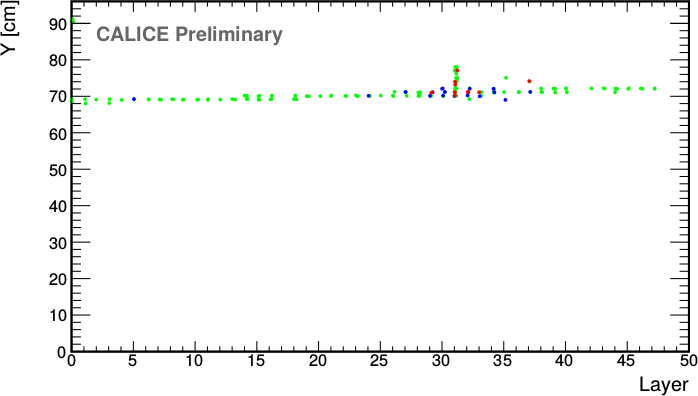
\includegraphics[width=.6\textwidth]{SDHCAL/figs/muon-rad.png}
      \caption{Exemple d'un muon radiatif de 50 $GeV$, enregistré par le prototype du SDHCAL sur la ligne H6 du SPS au CERN. Les couleurs indiquent les différents seuils de lecture.}
      \label{fig:muon-rad}
    \end{center}
  \end{figure}
\end{enumerate}
\begin{figure}[!ht]
  \begin{center}
    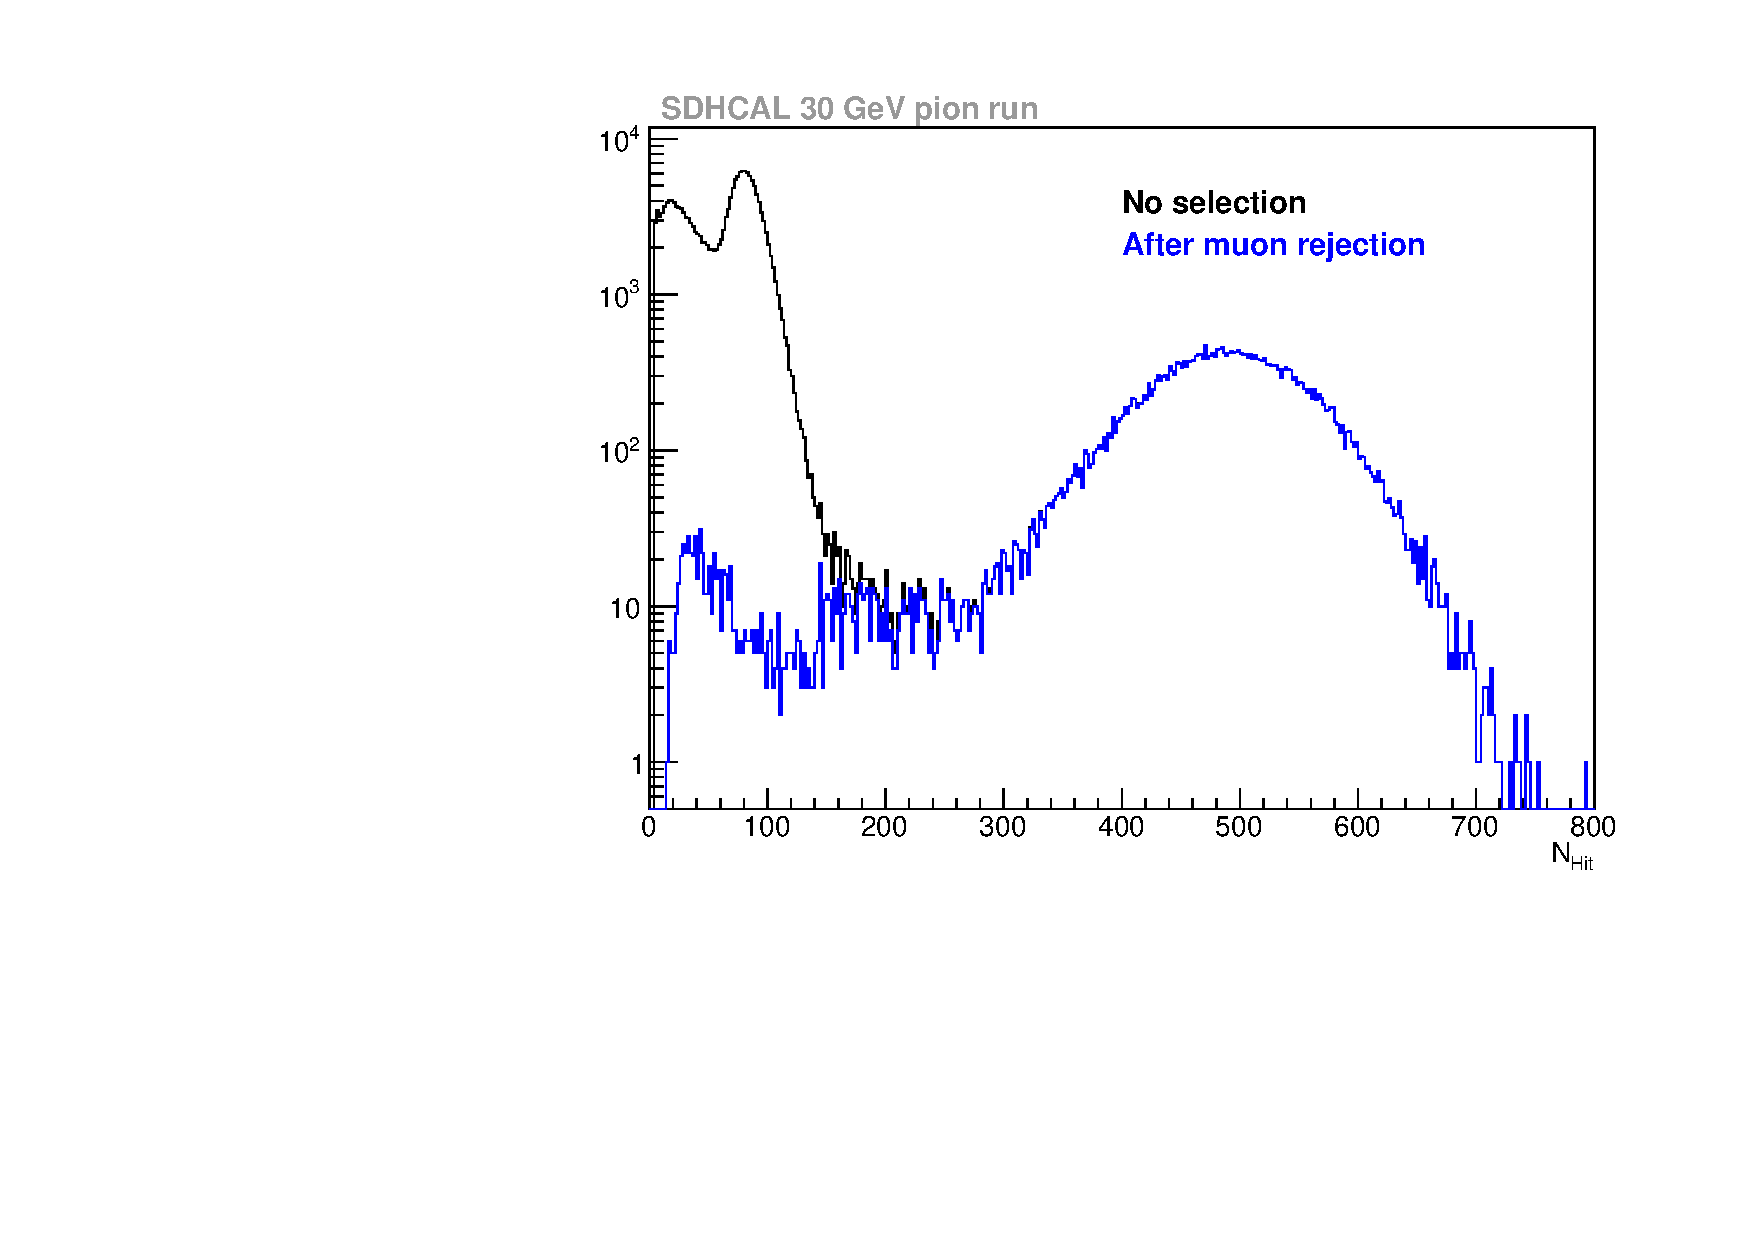
\includegraphics[width=.8\textwidth]{SDHCAL/figs/muCut715747.pdf}
    \caption{Distribution du nombre de hits avant (en noir) et après (en bleu) l'application des coupures pour rejeter les événements muons à 30 GeV.}
    \label{fig:muCut}
  \end{center}
\end{figure}
La figure~\ref{fig:muCut} montre la distribution du nombre de hits pour un échantillon de données à 30 GeV, avant et après l'application des coupures pour rejeter les muons.
\subsubsection{Contamination par les gerbes électromagnétiques}
Pour supprimer les événements induits par des électrons, au moins une des trois coupures suivantes doit être vérifiée:
\begin{enumerate}[-]
\item $N_{Traces}>0$, où $N_{Traces}$ correspond au nombre de traces reconstruites en utilisant la technique de Transformée de Hough (cf. section~\ref{sec.hough} du chapitre~\ref{chap.topo}). Si une trace reconstruite débute dans les trois premiers plans et que l'angle entre cette trace et l'axe $(Oz)$ est faible (<25$\degree$), alors elle définit la trace primaire;
\item $P_{Start}\geq5$, où $P_{Start}$ correspond au premier plan d’interaction. Il est défini comme étant le premier plan avec un amas avec plus de 4 hits. Ce plan doit se trouver après le dernier plan de la trace primaire. Le barycentre de l'amas de hits correspondant doit être situé à moins de 10 $cm$ de l'impact attendue de la trace primaire. Si aucune trace primaire n'est reconstruite, alors le premier plan avec un amas de plus de 4 hits proche de l'axe de la gerbe, définit le premier plan d’interaction;
\item $N_{Plans}>30$, les gerbes électromagnétiques sont très compactes. La valeur de la coupure a été optimisée avec la simulation puis vérifiée avec les données.
\end{enumerate}
\begin{figure}[!ht]
  \subfigure[]{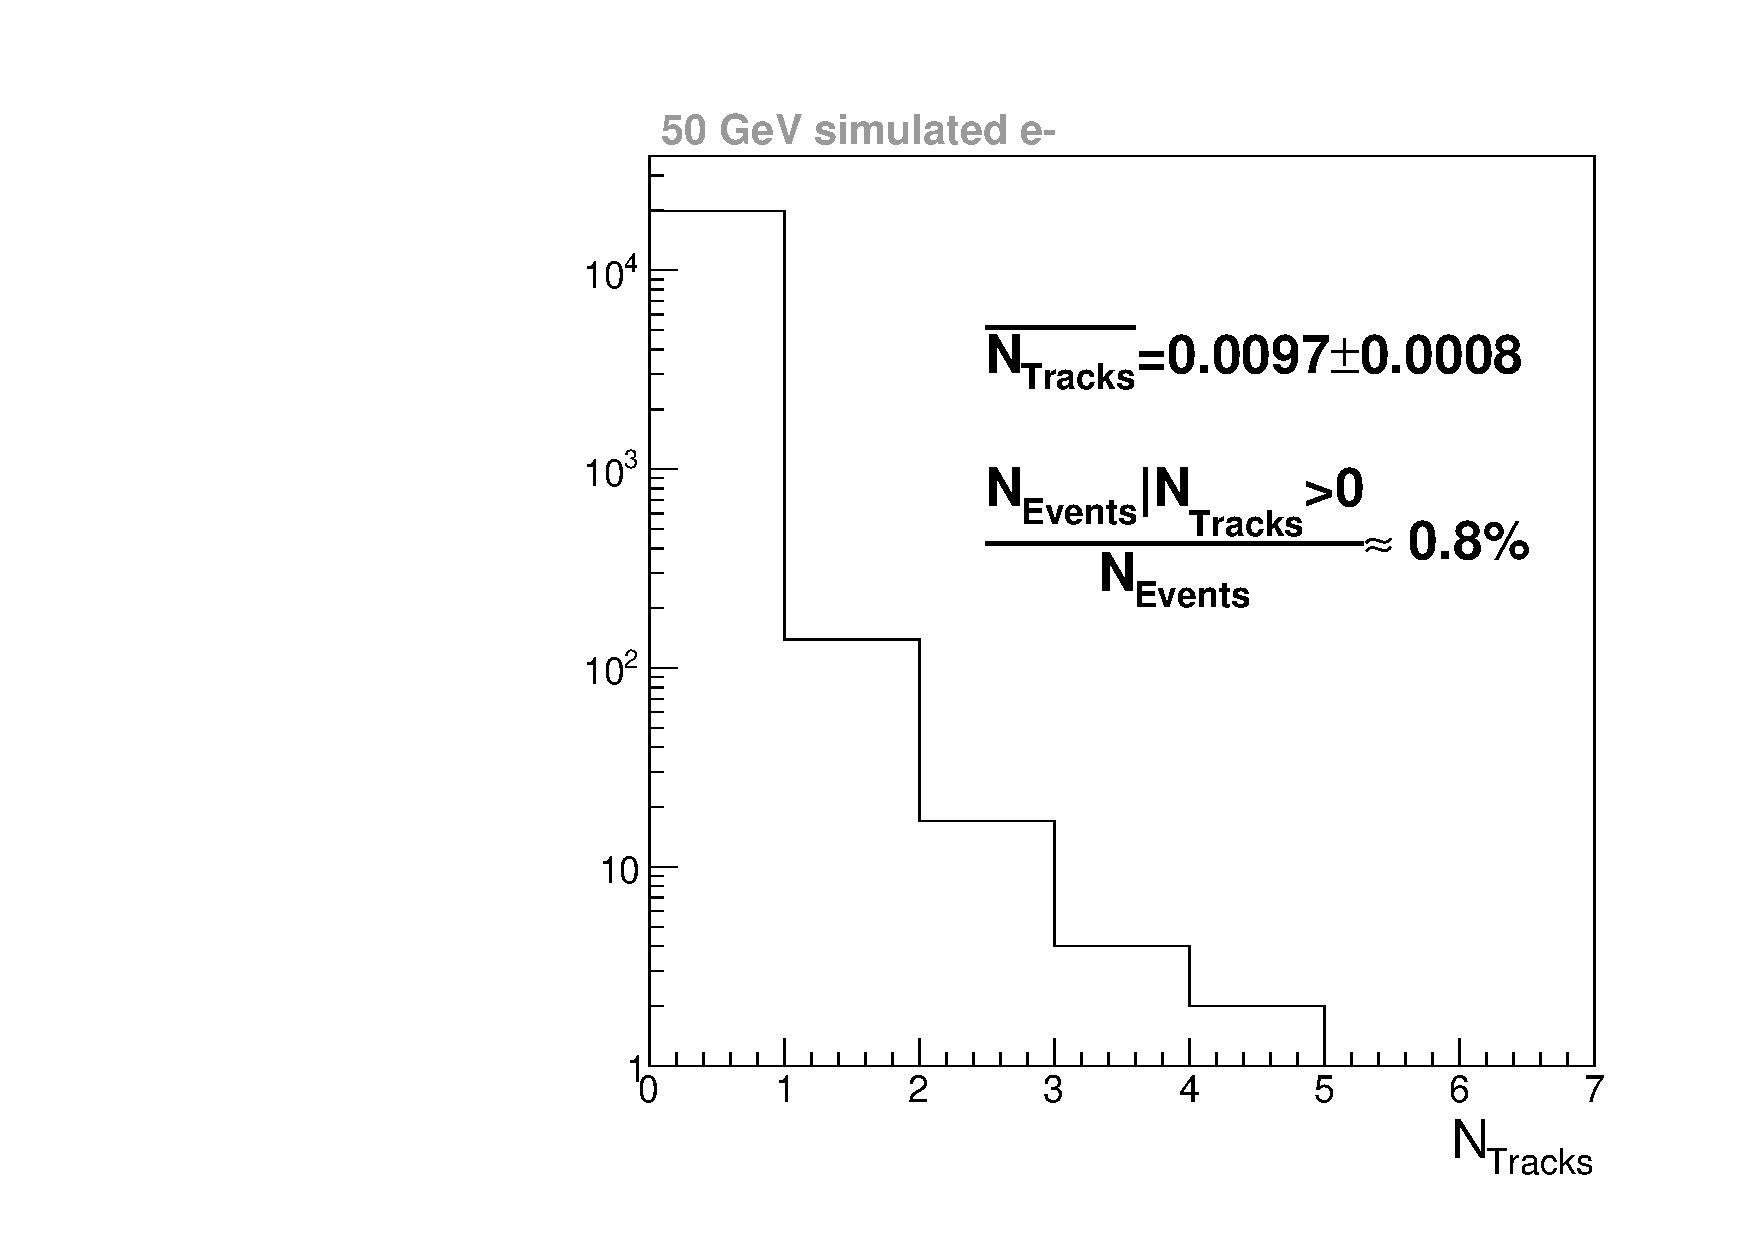
\includegraphics[width=.3\textwidth]{SDHCAL/figs/ntrack_e-_50GeV.pdf}}
  \subfigure[]{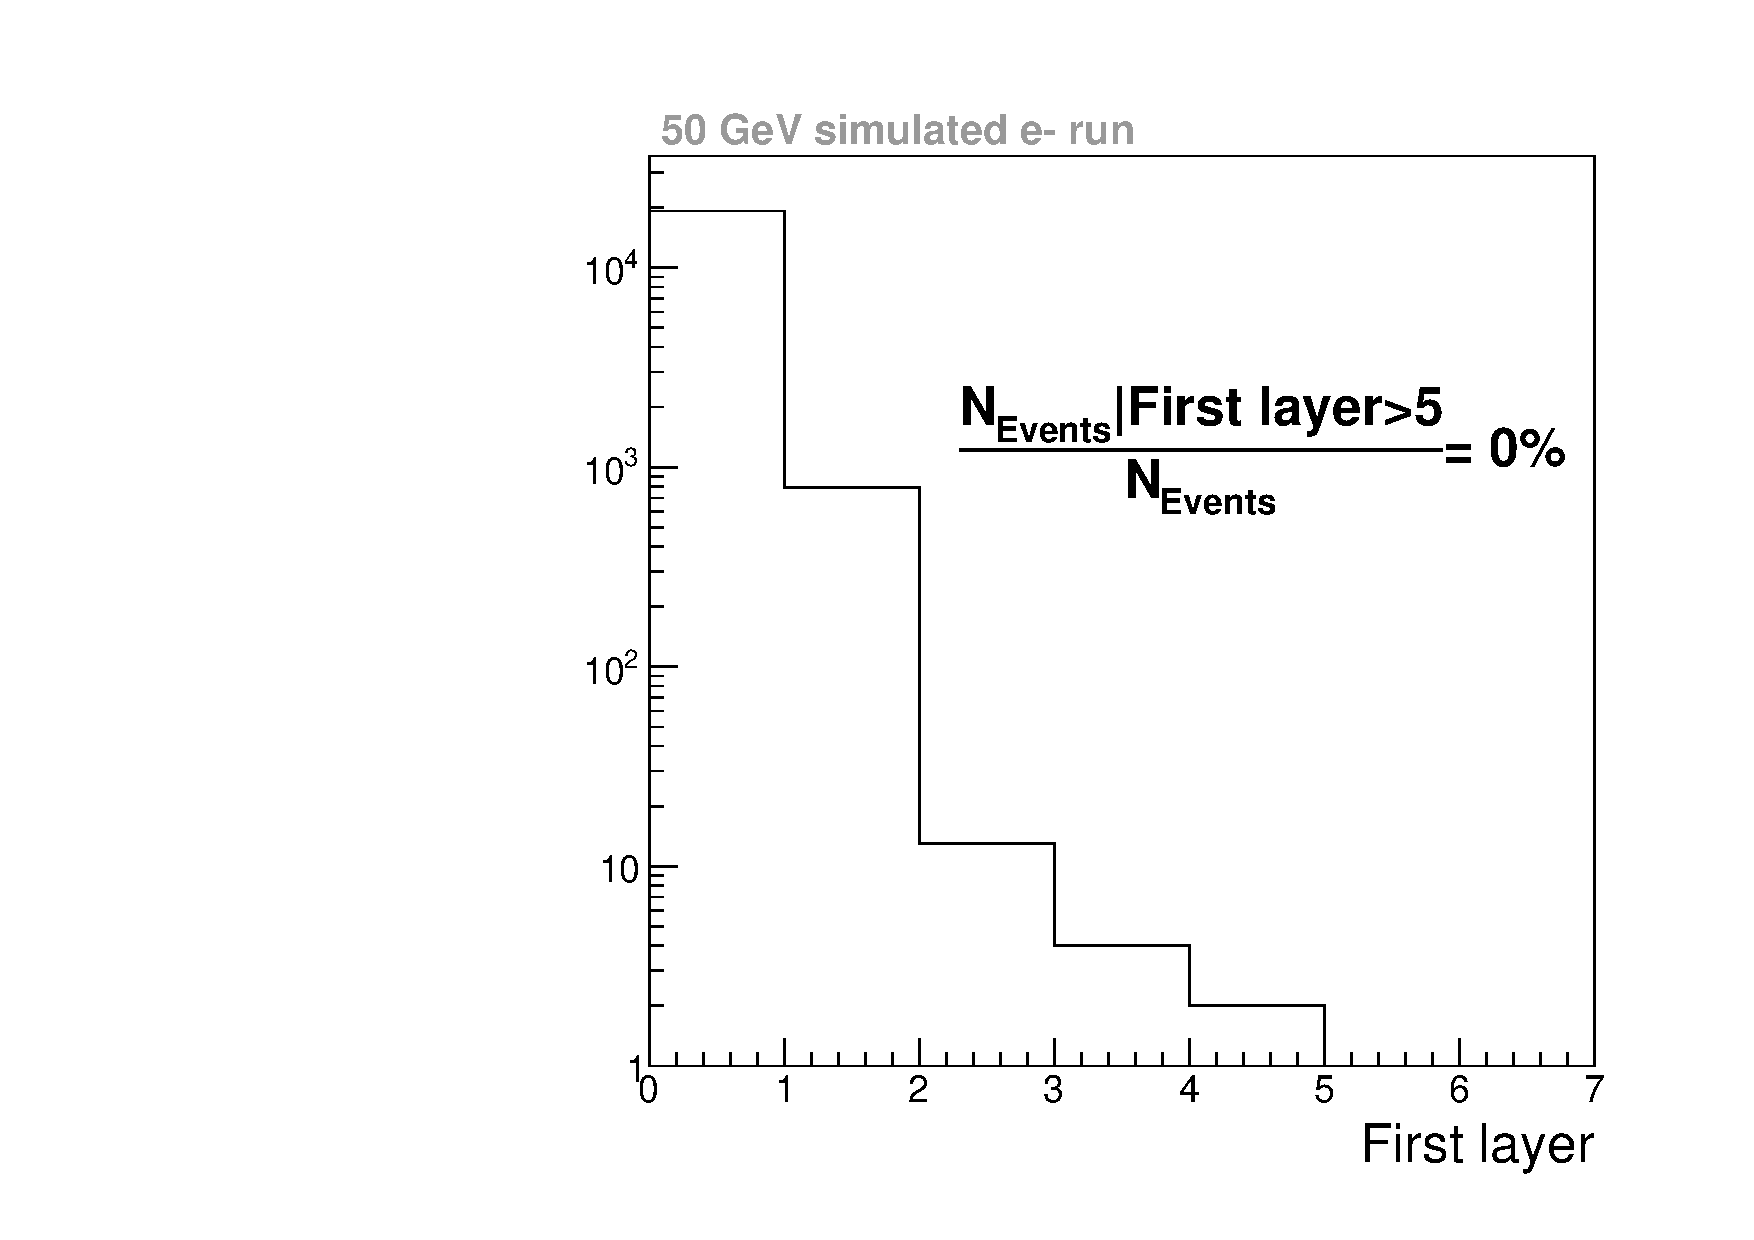
\includegraphics[width=.3\textwidth]{SDHCAL/figs/zbegin_e-_50GeV.pdf}}
  \subfigure[]{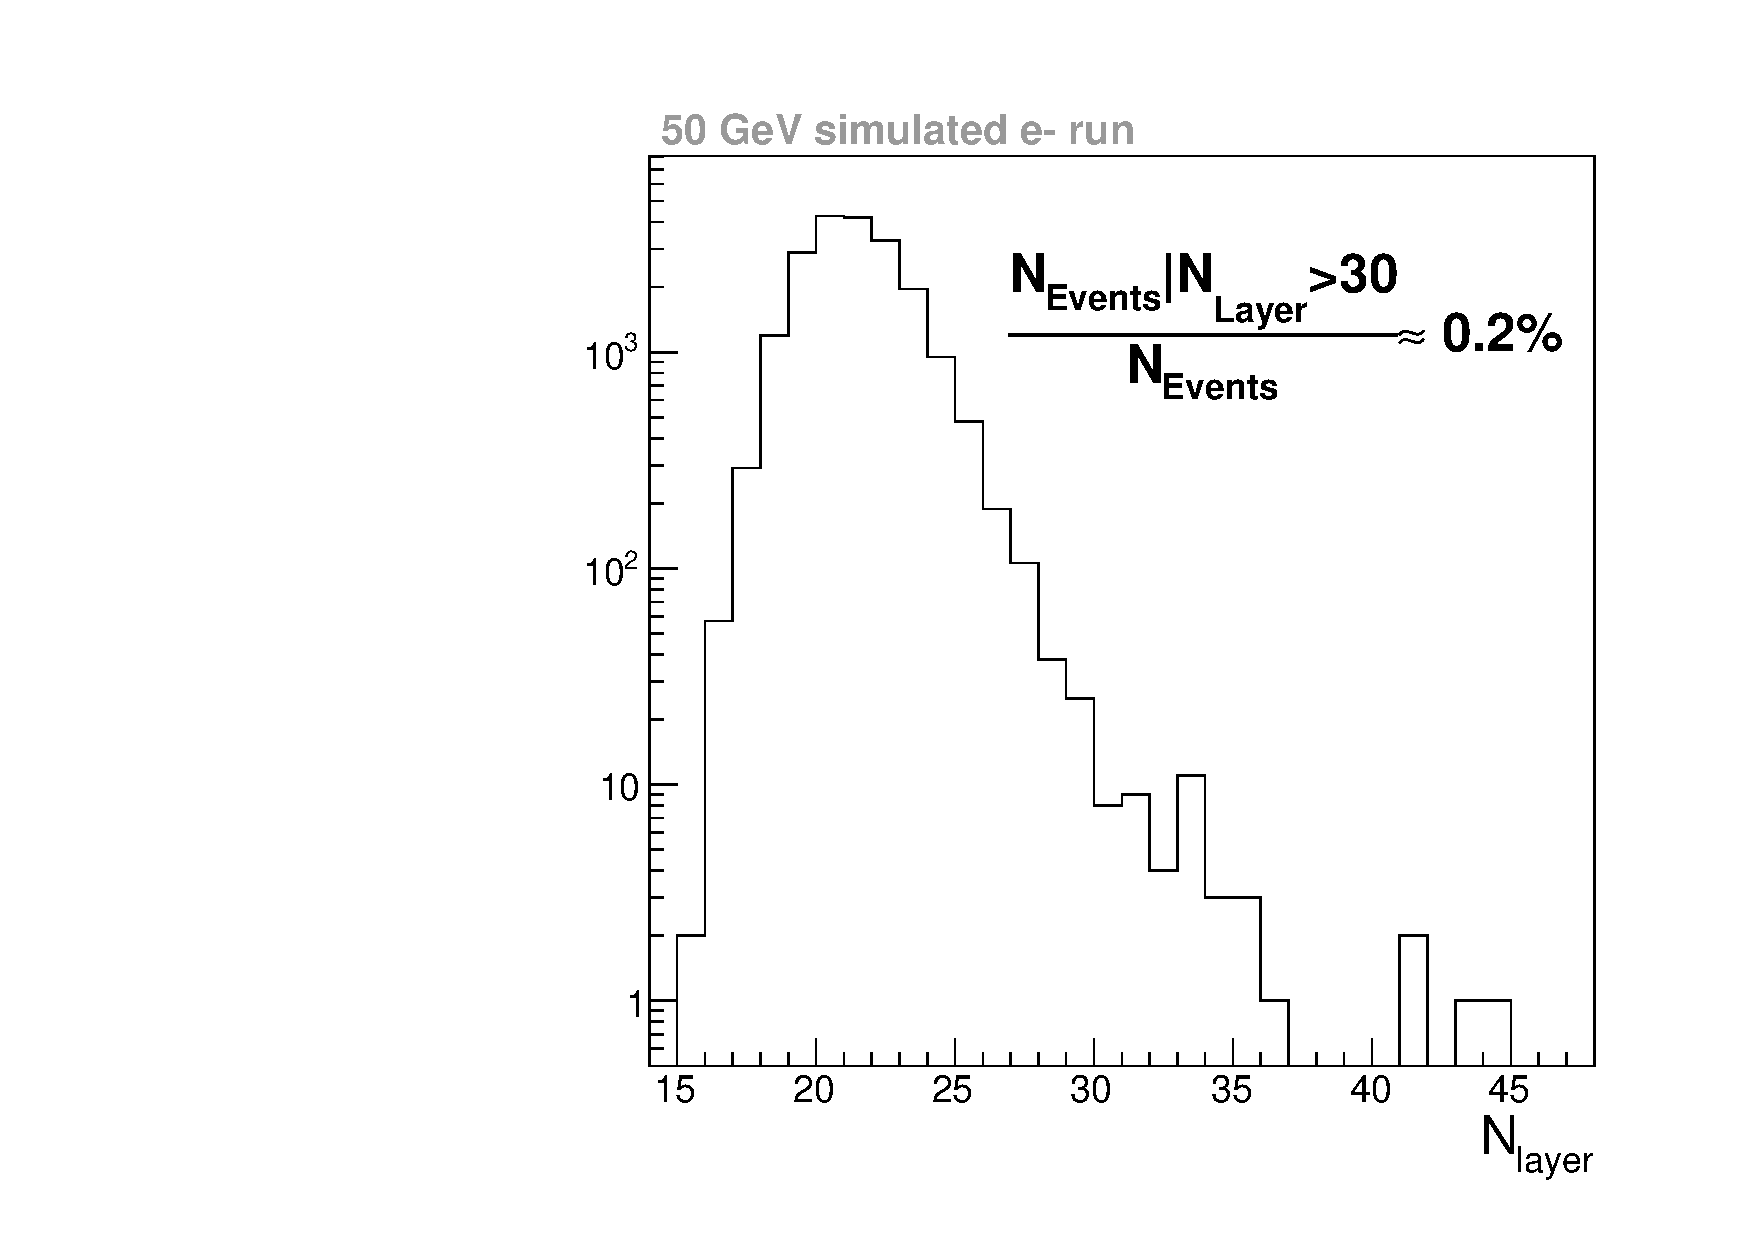
\includegraphics[width=.3\textwidth]{SDHCAL/figs/nlayer_e-_50GeV.pdf}}
  \caption{Distributions du nombre de traces reconstruites (a), du premier plan d'interaction (b) et du nombre de plans touchés (c) pour un échantillon de simulation de gerbes électromagnétiques à 50 $GeV$.\label{fig:electron_control}}
\end{figure}
La figure~\ref{fig:electron_control} montre les distributions des trois variables utilisées pour rejeter les électrons. Ces distributions proviennent de simulation d'électrons à 50 $GeV$. Pour chacune des variables, les rapports $\frac{N_{Events}|Var>cut}{N_{Events}}$ donnent la proportion d'événements non rejetés par les coupures définies ci-dessus. Ces rapports permettent d'affirmer que la proportion de gerbes électromagnétiques identifiées comme gerbes hadroniques, sera faible. Ces coupures sont toutes très efficaces pour filtrer les gerbes électromagnétiques mais elles sont combinées pour éviter de supprimer une partie significative des gerbes hadroniques et ainsi de biaiser nos échantillons de données. Notons que pendant les tests en faisceau, une fine couche de plomb (8 $mm$ d'épaisseur) était insérée sur la ligne de faisceau pour diminuer la contamination par les électrons. 
\subsubsection{Coupures supplémentaires}
La figure~\ref{fig:muCut} montre que les échantillons de données sont toujours contaminés, notamment dans la région de faible nombre de hits, malgré les coupures déjà appliquées. Quelques coupures supplémentaires sont nécessaires pour purifier les échantillons de données:
\begin{enumerate}[-]
\item les événements multiples sont filtrés en étudiant la dispersion des hits dans les 5 premiers plans. Ces événements sont issus la plupart du temps d’interactions de la particule incidente en amont du prototype (interactions avec les collimateurs, la couche de plomb, avec les détecteurs permettant le réglage du faisceau...). Si des amas de hits sont séparés de plus de 5 $cm$ dans 4 des 5 premiers plans alors l'événement est considéré comme multiple. La figure~\ref{fig:multiple} montre un exemple d'événement identifié comme multiple dans le prototype du SDHCAL;
  \begin{figure}[!ht]
    \begin{center}
      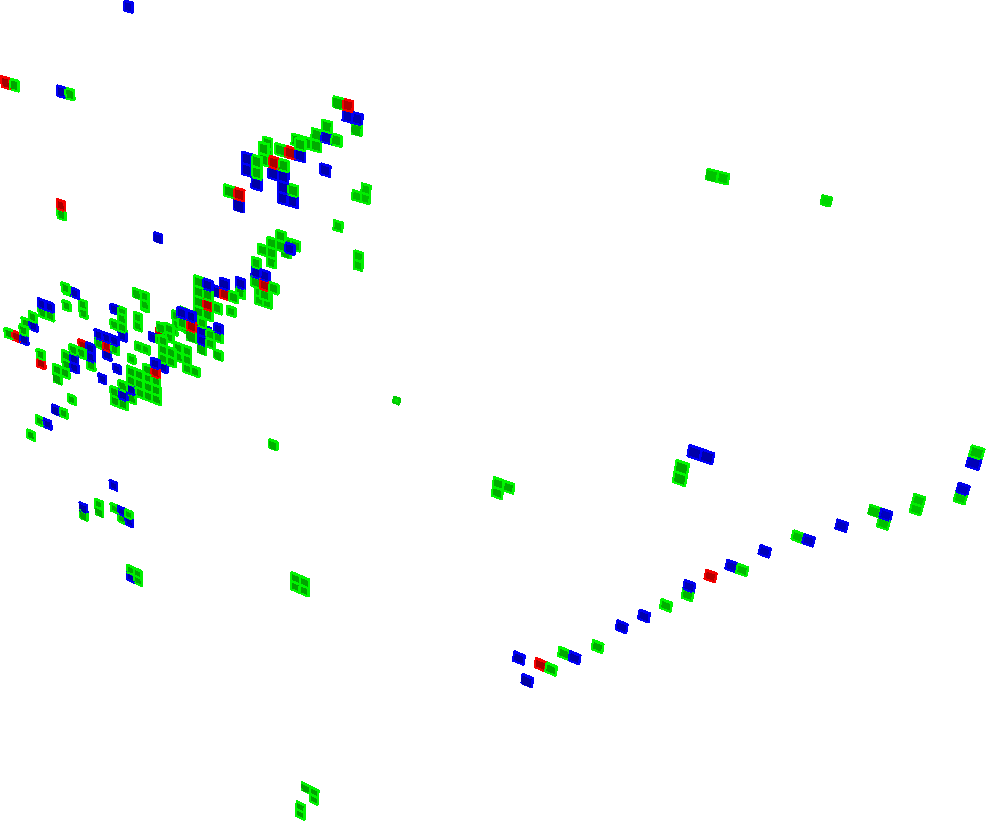
\includegraphics[width=.5\textwidth]{SDHCAL/figs/multiple.png}
      \caption{Exemple d'événement multiple, enregistré par le prototype du SDHCAL sur la ligne H6 du SPS au CERN. Les couleurs indiquent les différents seuils de lecture.}
      \label{fig:multiple}
    \end{center}
  \end{figure}
\item les particules neutres sont filtrées en imposant la présence d'au moins 4 hits dans les 5 premiers plans. Cette coupures rejette aussi beaucoup de muons cosmiques;
\item l'angle entre la particule incidente et l'axe $(Oz)$ doit être inférieur à 25$\degree$. Cette coupure permet aussi d'éliminer des événements où la particule incidente aurait légèrement interagit avant le prototype.
\end{enumerate}
\label{sec.shower_selection}
\begin{figure}[!ht]
  \begin{center}
    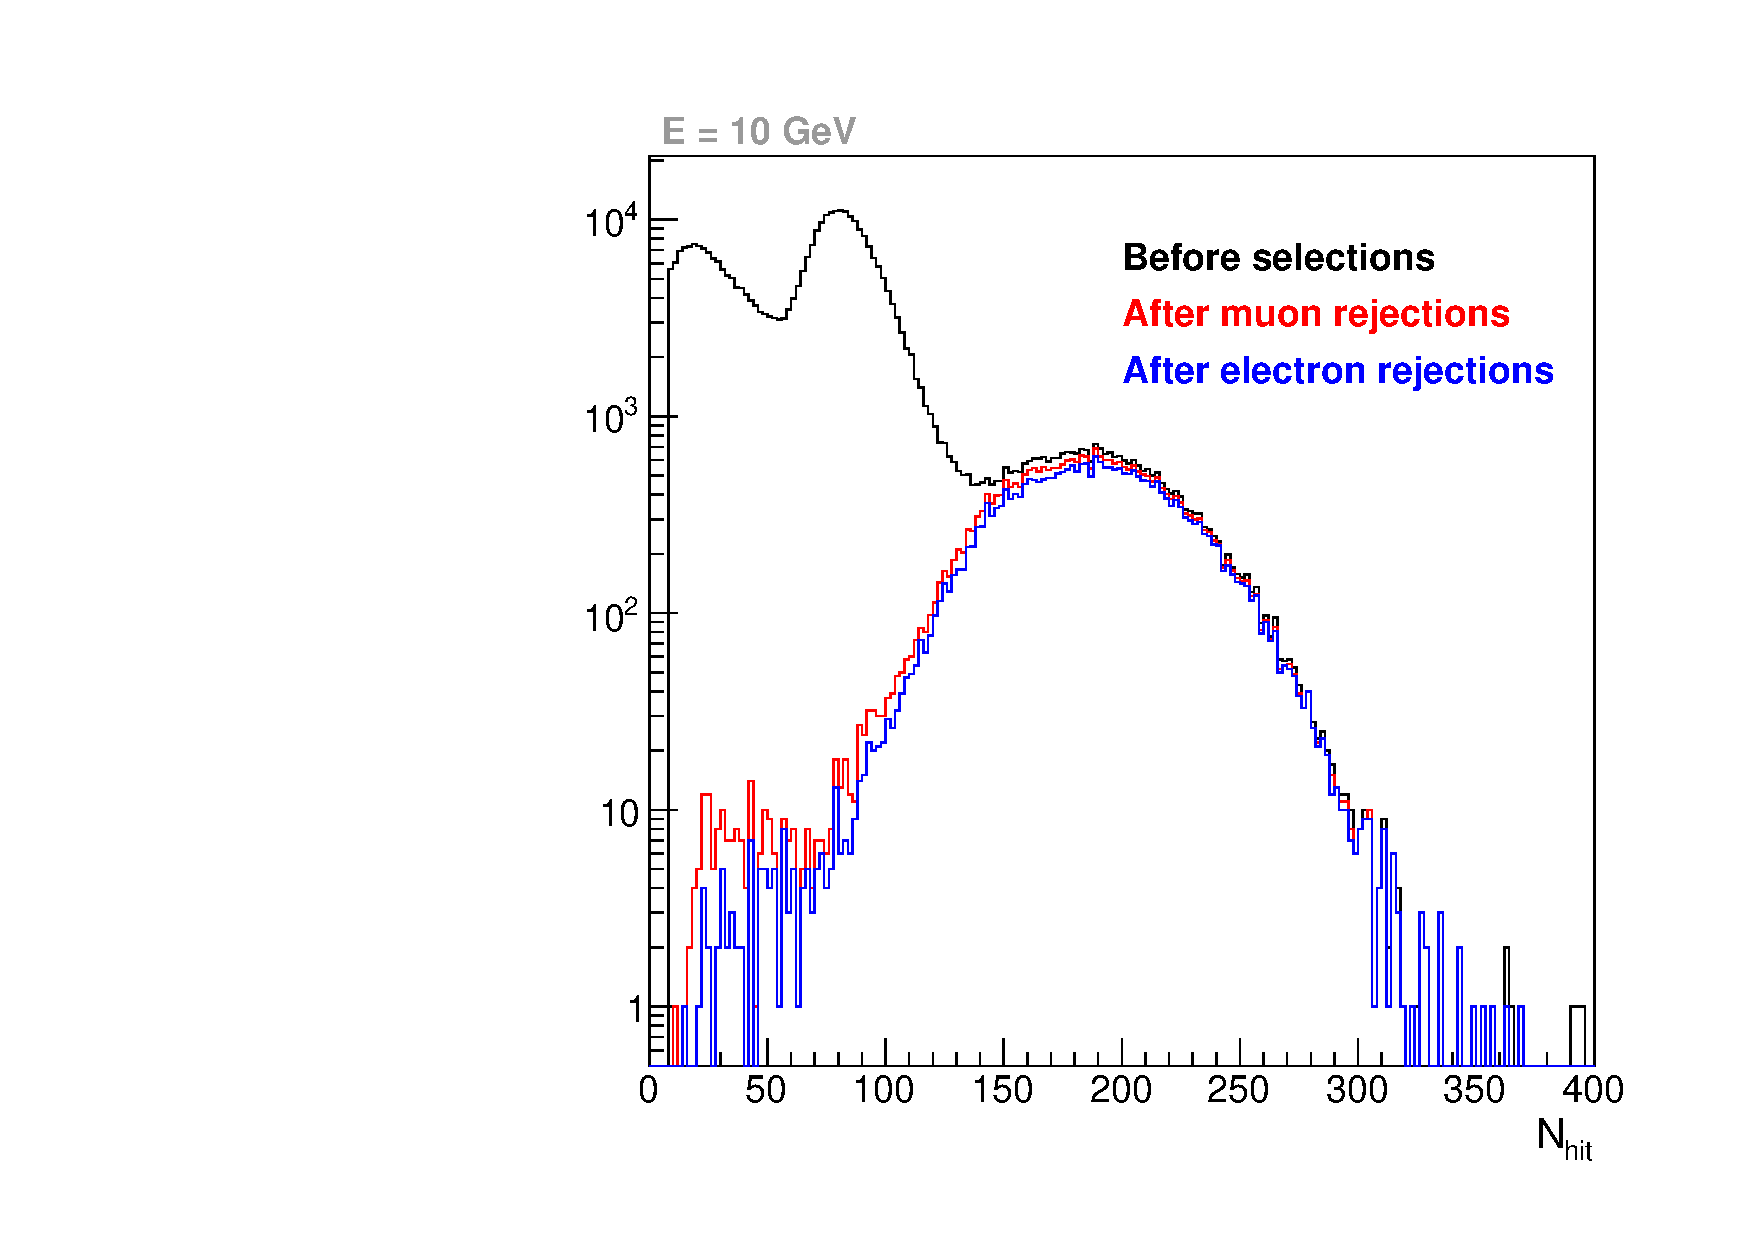
\includegraphics[width=.45\textwidth]{SDHCAL/figs/pi-_selection10GeV.pdf}
    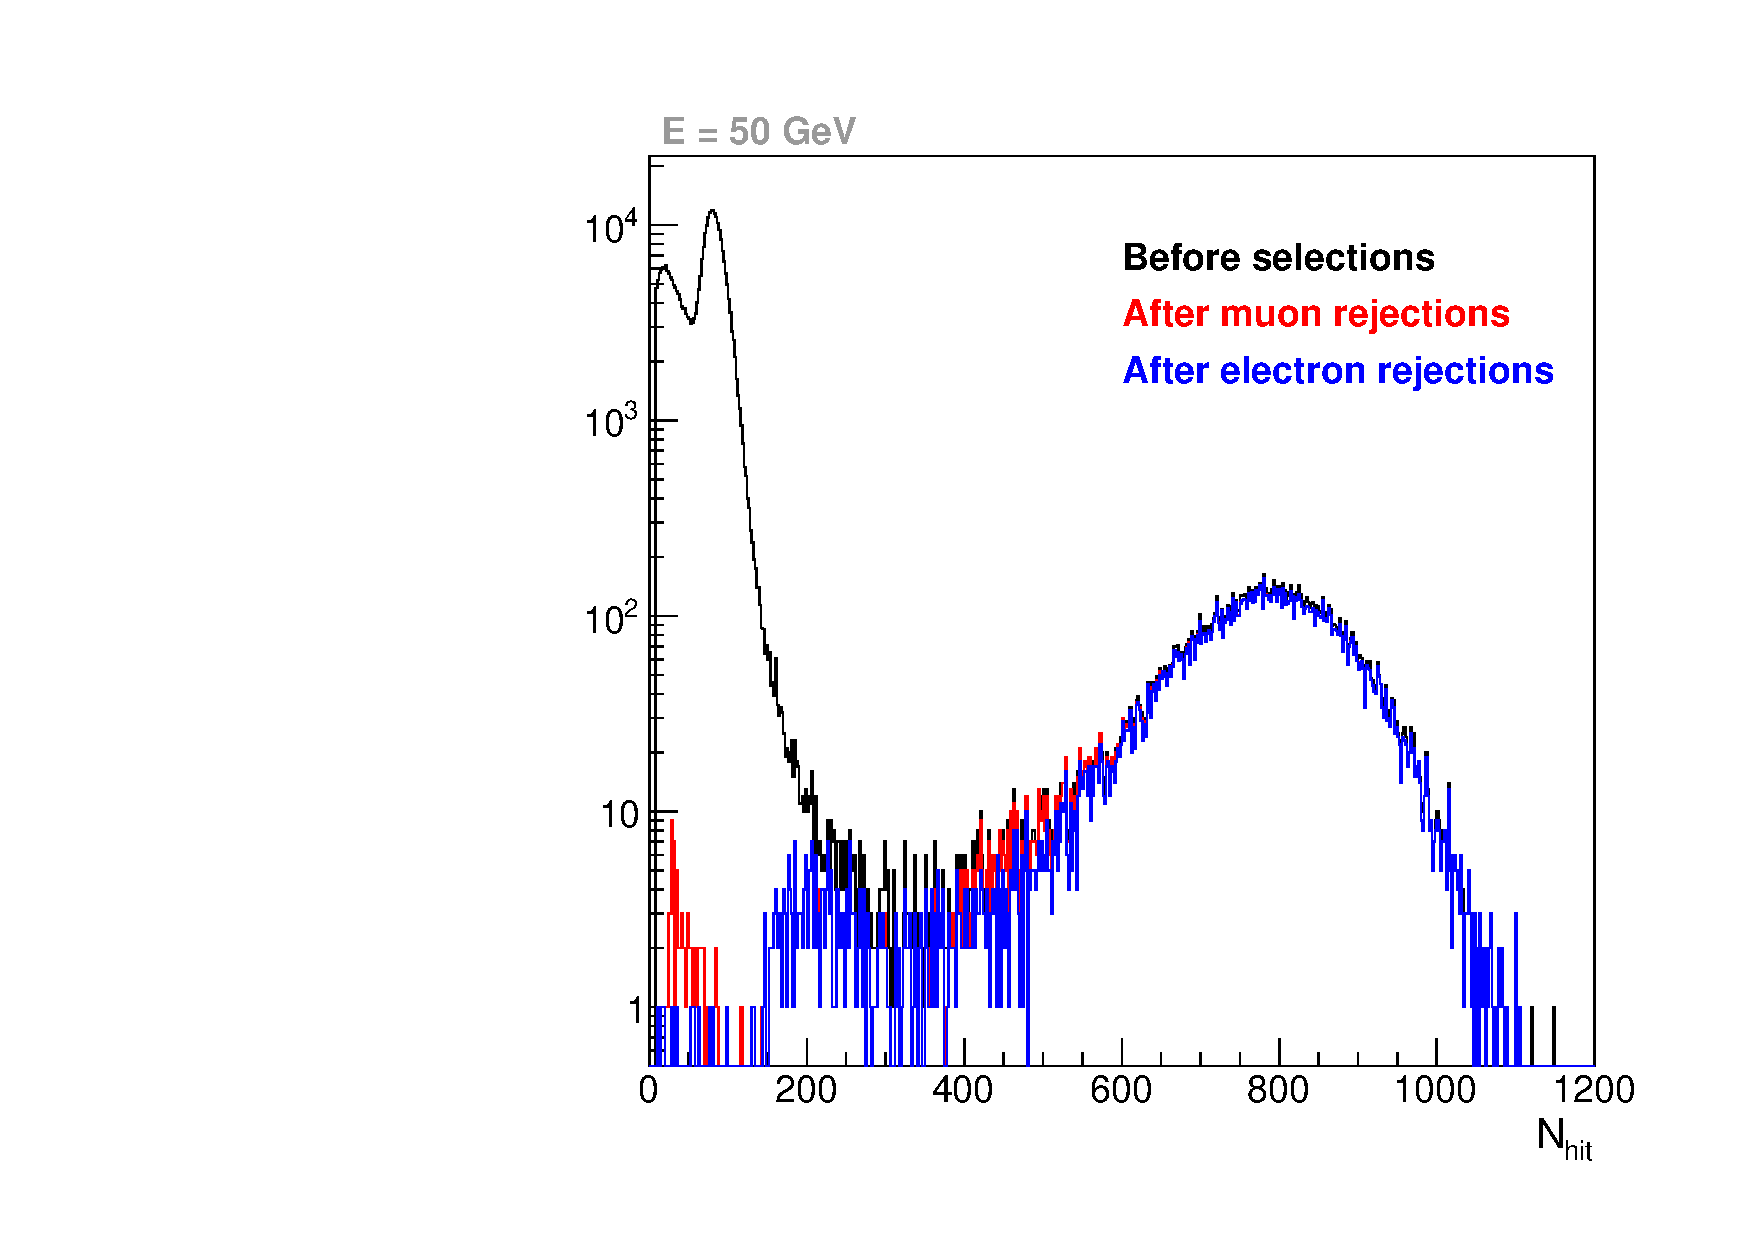
\includegraphics[width=.45\textwidth]{SDHCAL/figs/pi-_selection50GeV.pdf}
    \caption{Distribution du nombre de hits pour des échantillons de données à 10 (à gauche) et 50 (à droite) $GeV$ avant toutes les coupures (en noir), après les coupures de sélection des gerbes hadroniques (en bleu) et après les coupures de sélection des gerbes électromagnétiques (en rouge).}
    \label{fig:pion_selection}
  \end{center}
\end{figure}
La figure~\ref{fig:pion_selection} présente les distributions de nombre de hits pour des échantillons de données à 10 et 50 $GeV$ avant toutes les coupures (en noir), et après les coupures pour filtrer les muons (en rouge), puis les électrons (en bleu). Nous détaillerons la procédure de sélection des électrons dans la section~\ref{sec.resultats} du chapitre~\ref{chap.simulation}. Les coupures que nous venons de détailler ont été accordées pour purifier au maximum les échantillons de données tout en essayant de conserver un maximum de gerbes hadroniques et ainsi d'introduire un minimum de biais.
\begin{table}[!ht]
  \begin{center}
    \begin{tabular}{c|c}
      \rowcolor{black!20!white}Energie & Efficacité \\
      \rowcolor{black!5!white}\hline
      \rowcolor{black!5!white}$5 ~GeV$ & $57.9\pm0.3\%$  \\
      \rowcolor{black!5!white}$10~GeV$ & $85.8\pm0.2\%$ \\
      \rowcolor{black!5!white}$15~GeV$ & $90.5\pm0.2\%$ \\
      \rowcolor{black!5!white}$20~GeV$ & $92.3\pm0.2\%$ \\
      \rowcolor{black!5!white}$25~GeV$ & $93.9\pm0.2\%$ \\
      \rowcolor{black!5!white}$30~GeV$ & $94.3\pm0.2\%$ \\
      \rowcolor{black!5!white}$40~GeV$ & $95.1\pm0.2\%$ \\
      \rowcolor{black!5!white}$50~GeV$ & $94.9\pm0.2\%$ \\
      \rowcolor{black!5!white}$60~GeV$ & $95.1\pm0.2\%$ \\
      \rowcolor{black!5!white}$70~GeV$ & $94.5\pm0.2\%$ \\
      \rowcolor{black!5!white}$80~GeV$ & $94.3\pm0.2\%$ \\
    \end{tabular}
  \end{center}  
  \caption{Efficacité de sélection des gerbes hadroniques en fonction de l'énergie de la particule incidente.}
  \label{tab.pi-selection}
\end{table}
Le tableau~\ref{tab.pi-selection} présente l'efficacité de sélection des gerbes hadroniques en fonction de l'énergie incidente. Cette efficacité est mesurée avec la simulation et correspond au rapport entre le nombre d'événements simulés et le nombre d'événements identifiés comme gerbes hadroniques. Ces efficacités sont satisfaisantes excepté à 5 $GeV$. Environ 21$\%$ des gerbes hadroniques simulées à 5 $GeV$ sont rejetées par les coupures muons, 15 $\%$ par les coupures électrons et environ 11$\%$ sont rejetées à cause de la coupure sur l'angle de la gerbe. Ceci est dû au fait qu'à 5 $GeV$, la particule incidente subie le phénomène de diffusion multiple dans les couches d'absorbeurs. En comparaison, aucun événement de gerbe hadronique simulé à 80 $GeV$ n'est rejeté par cette coupure.
\subsection{Calibration en fonction du temps}
\label{sec.timeCalib}
Dans la section~\ref{sec.grpc} de ce chapitre, nous avons déjà expliqué que la résistivité des électrodes est un paramètre très important pour les RPC. La résistivité volumique du verre utilisé pour le SDHCAL est très élevée ($\rho=10^{12}~\Omega cm$). Cette résistivité élevée a pour conséquence de fortement dégrader l'efficacité de détection des GRPC lorsque le flux de particules augmente. La figure~\ref{fig:eff_vs_rate} présente l'efficacité de détection de différentes GRPC en fonction du flux de particules incidentes~\cite{haddad}. 
\begin{figure}[!ht]
  \begin{center}
    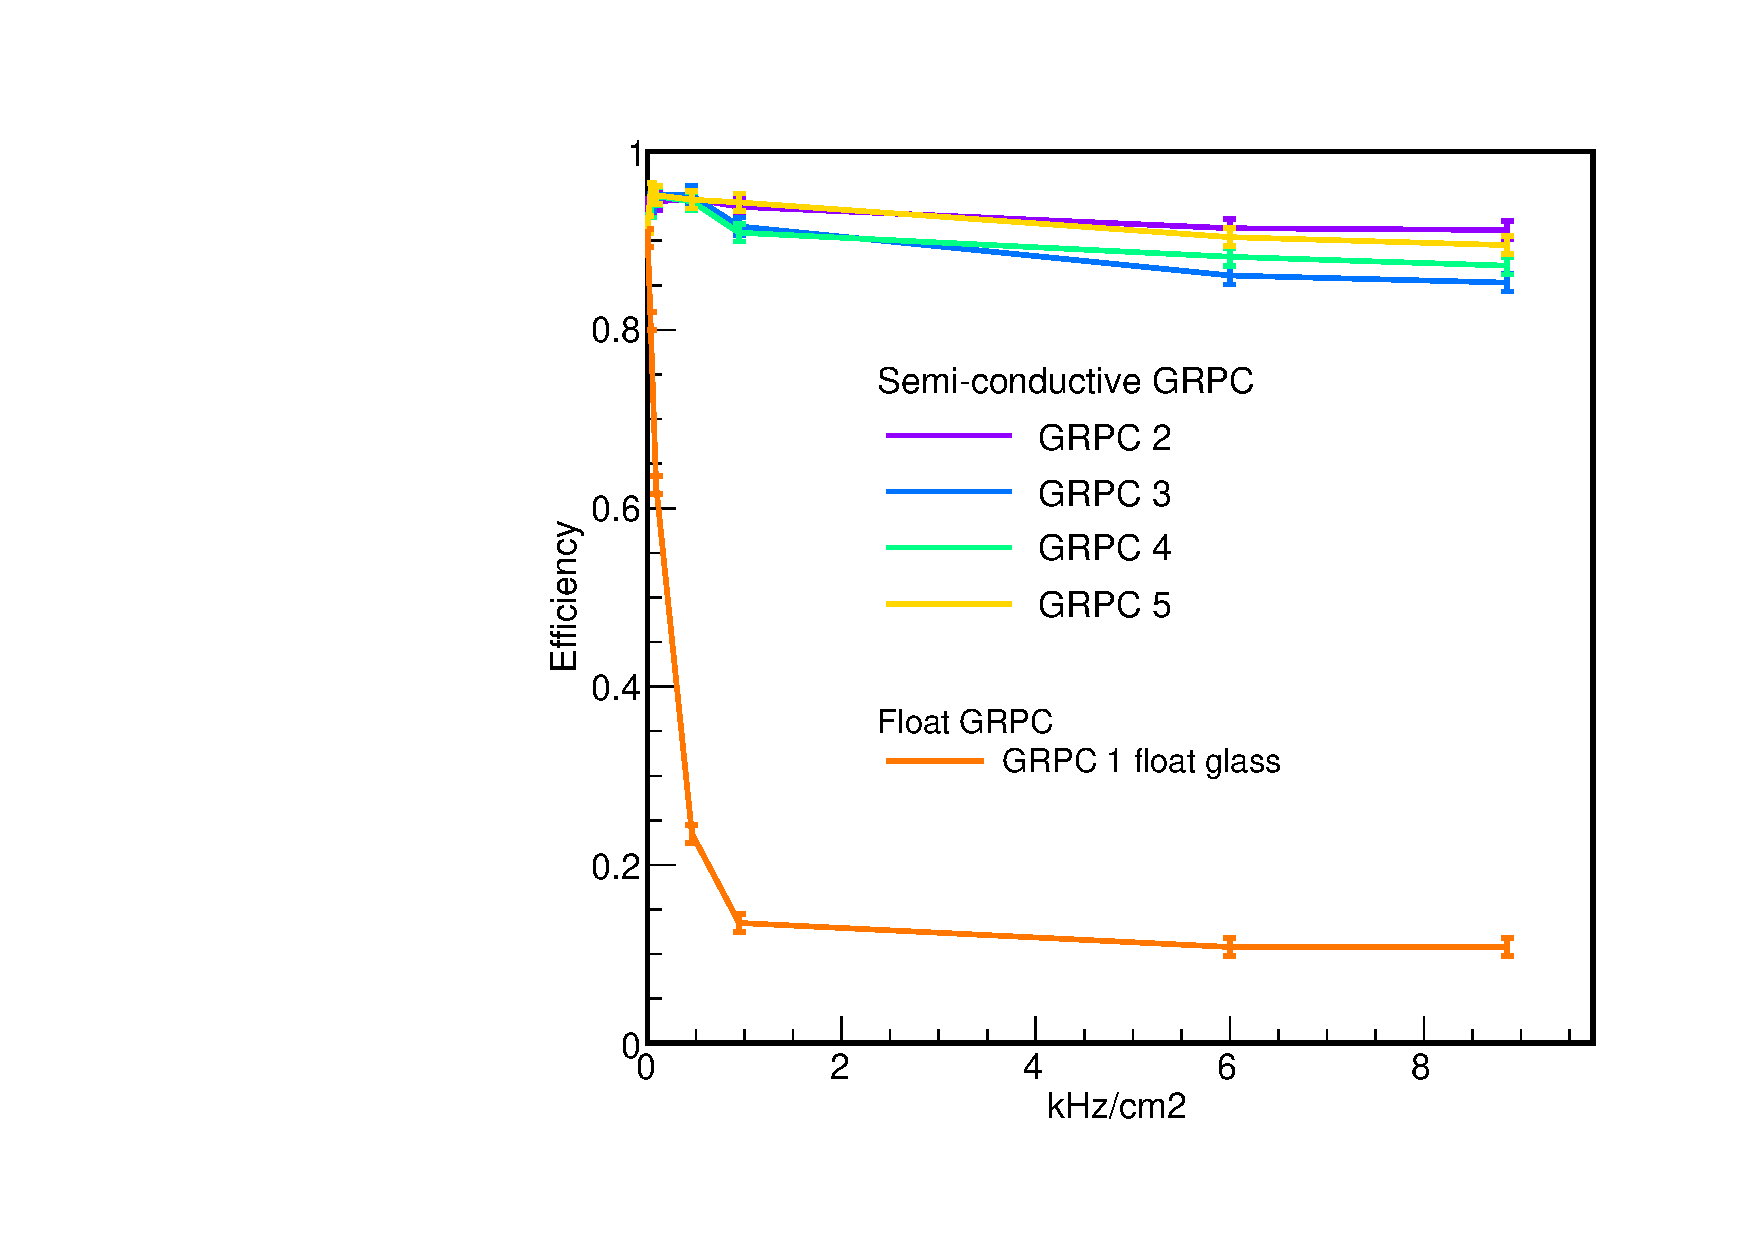
\includegraphics[width=.6\textwidth]{SDHCAL/figs/EFFRate.pdf}
    \caption{Efficacité de détection en fonction du flux de particules incidentes.}
    \label{fig:eff_vs_rate}
  \end{center}
\end{figure}
L'efficacité de la chambre avec du verre standard (Float Glass, courbe orange) chute très rapidement lorsque le taux augmente. Les GRPC construites avec du verre semi-conducteur, fabriqué à l'université de Tsinghua en Chine \cite{yi_wang}, ont une résistivité plus faible que les GRPC du SDHCAL ($\rho=10^{10}~\Omega cm$). Cette résistivité leur permet de conserver une bonne efficacité malgré un fort flux de particules.
Cet effet est encore plus important avec les gerbes hadroniques et électromagnétiques où la densité de particules secondaires est très élevée.
\begin{figure}[!ht]
  \begin{center}
    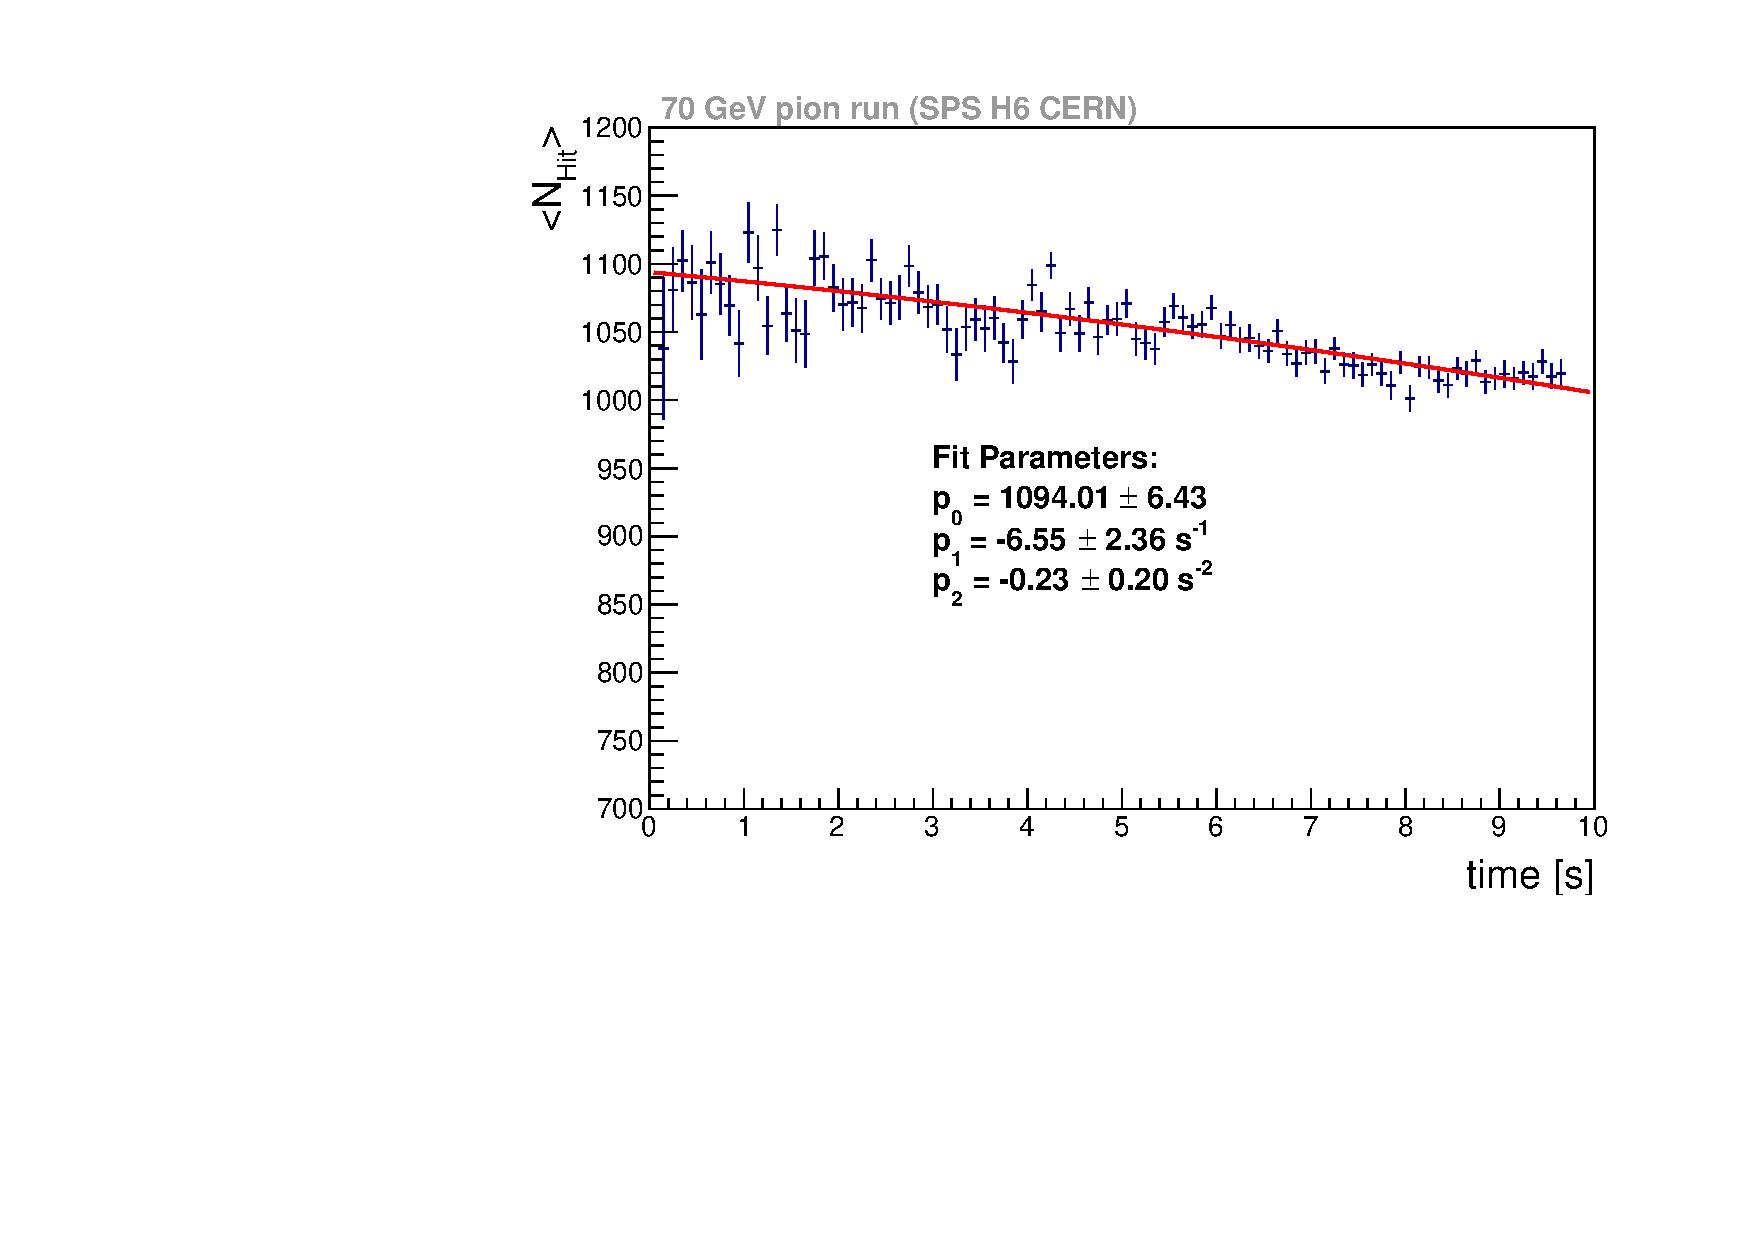
\includegraphics[width=.7\textwidth]{SDHCAL/figs/timeCalib70.pdf}
    \caption{Nombre moyen de hits pour des gerbes hadroniques de 70 $GeV$ en fonction du temps relatif au début d'un cycle du SPS.}
    \label{fig:time_correction}
  \end{center}
\end{figure}
La figure~\ref{fig:time_correction} montre le nombre moyen de hits pour des gerbes hadroniques de 70 $GeV$ en fonction du temps relatif au début d'un cycle du SPS en 2012. Pour construire cette figure, le temps relatif au début du cycle du SPS est reconstruit pendant l'analyse des données en imposant le début d'un nouveau cycle lorsque plus de cinq secondes s'écoulent entre deux événements consécutifs. Le nombre de hits décroit sensiblement avec le temps. Cet effet augmente avec l'énergie du faisceau. En effet, à plus haute énergie, le nombre de particules secondaires augmente et donc la charge déposée sur les électrodes. Le temps pour neutraliser ces charges est donc légèrement plus long. Une procédure de calibration permet cependant de corriger cet effet. Les courbes de nombre de hits en fonction du temps, pour chaque seuil, sont ajustées avec un polynôme d'ordre 2. Le nombre de hits pour chaque seuil, pour chaque événement, est corrigé en utilisant le résultats de l'ajustement:
\begin{equation}
  N_{corr,i}=N_i-\sum_{j=0}^{2}p_{j,i}t^j
\end{equation}
où $i$ correspond au seuil, $N_i$ est le nombre de hits et $N_{corr,i}$ le nombre de hits corrigé pour le seuil $i$, les $p_{j,i}$ sont les coefficients de correction obtenus avec les ajustements et $t$ est le temps relatif au début du cycle du SPS.
\begin{figure}[!ht]
  \begin{center}
    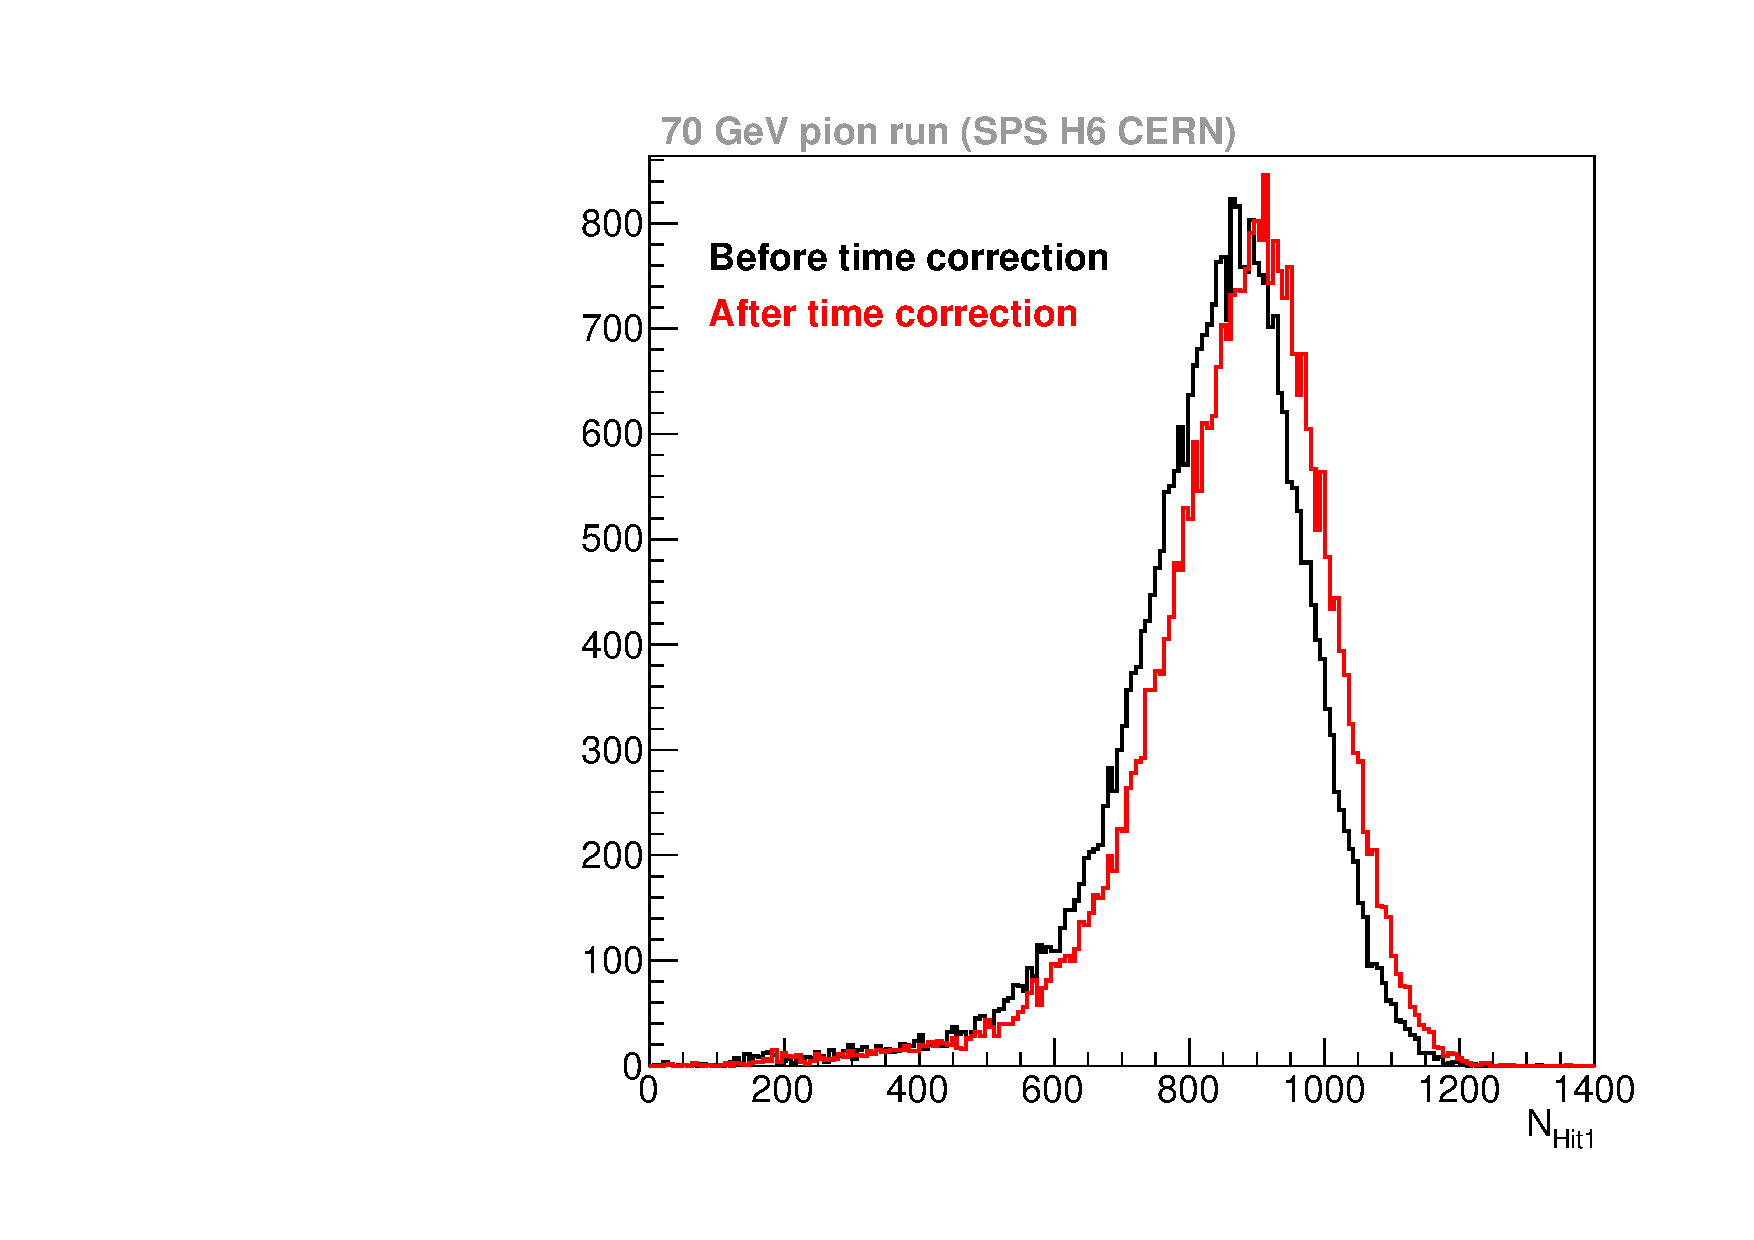
\includegraphics[width=.32\textwidth]{SDHCAL/figs/time_corr1.pdf}
    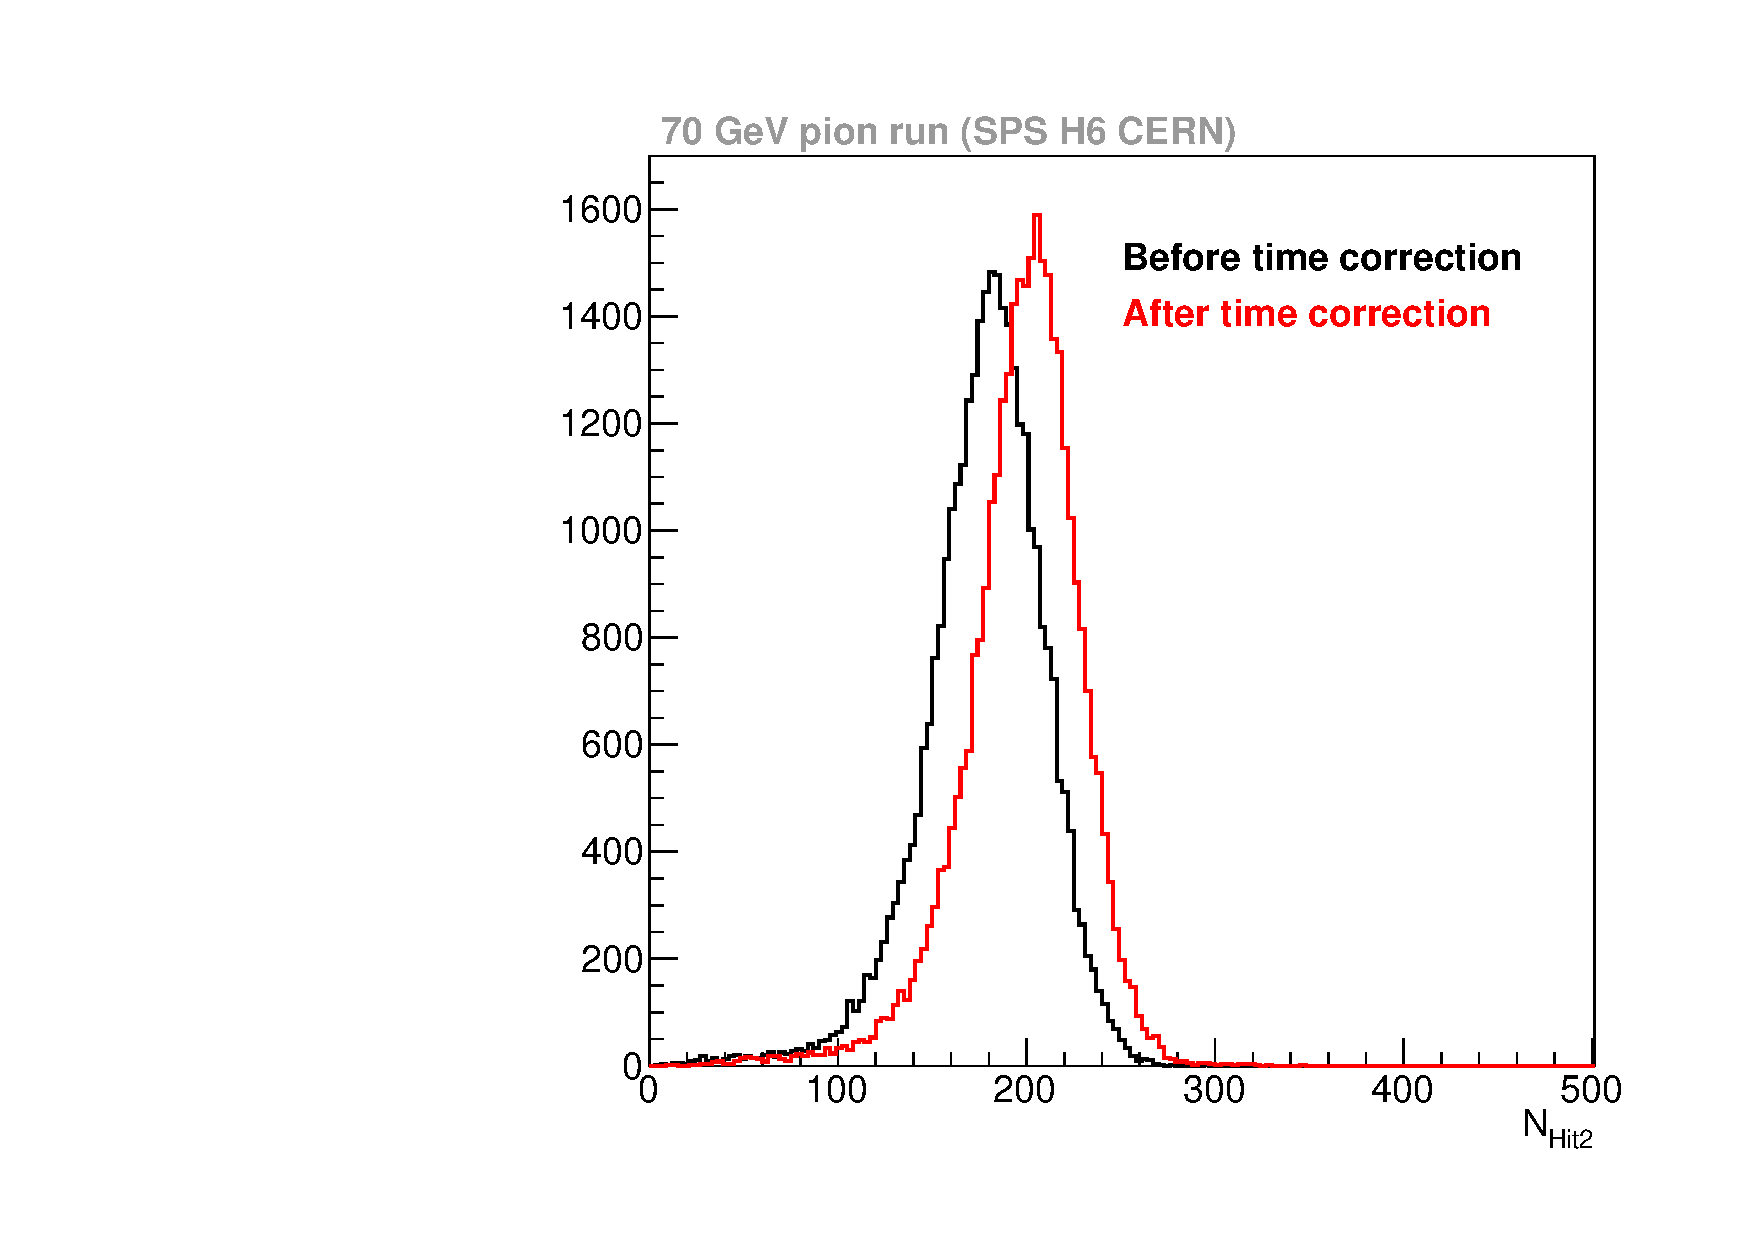
\includegraphics[width=.32\textwidth]{SDHCAL/figs/time_corr2.pdf}
    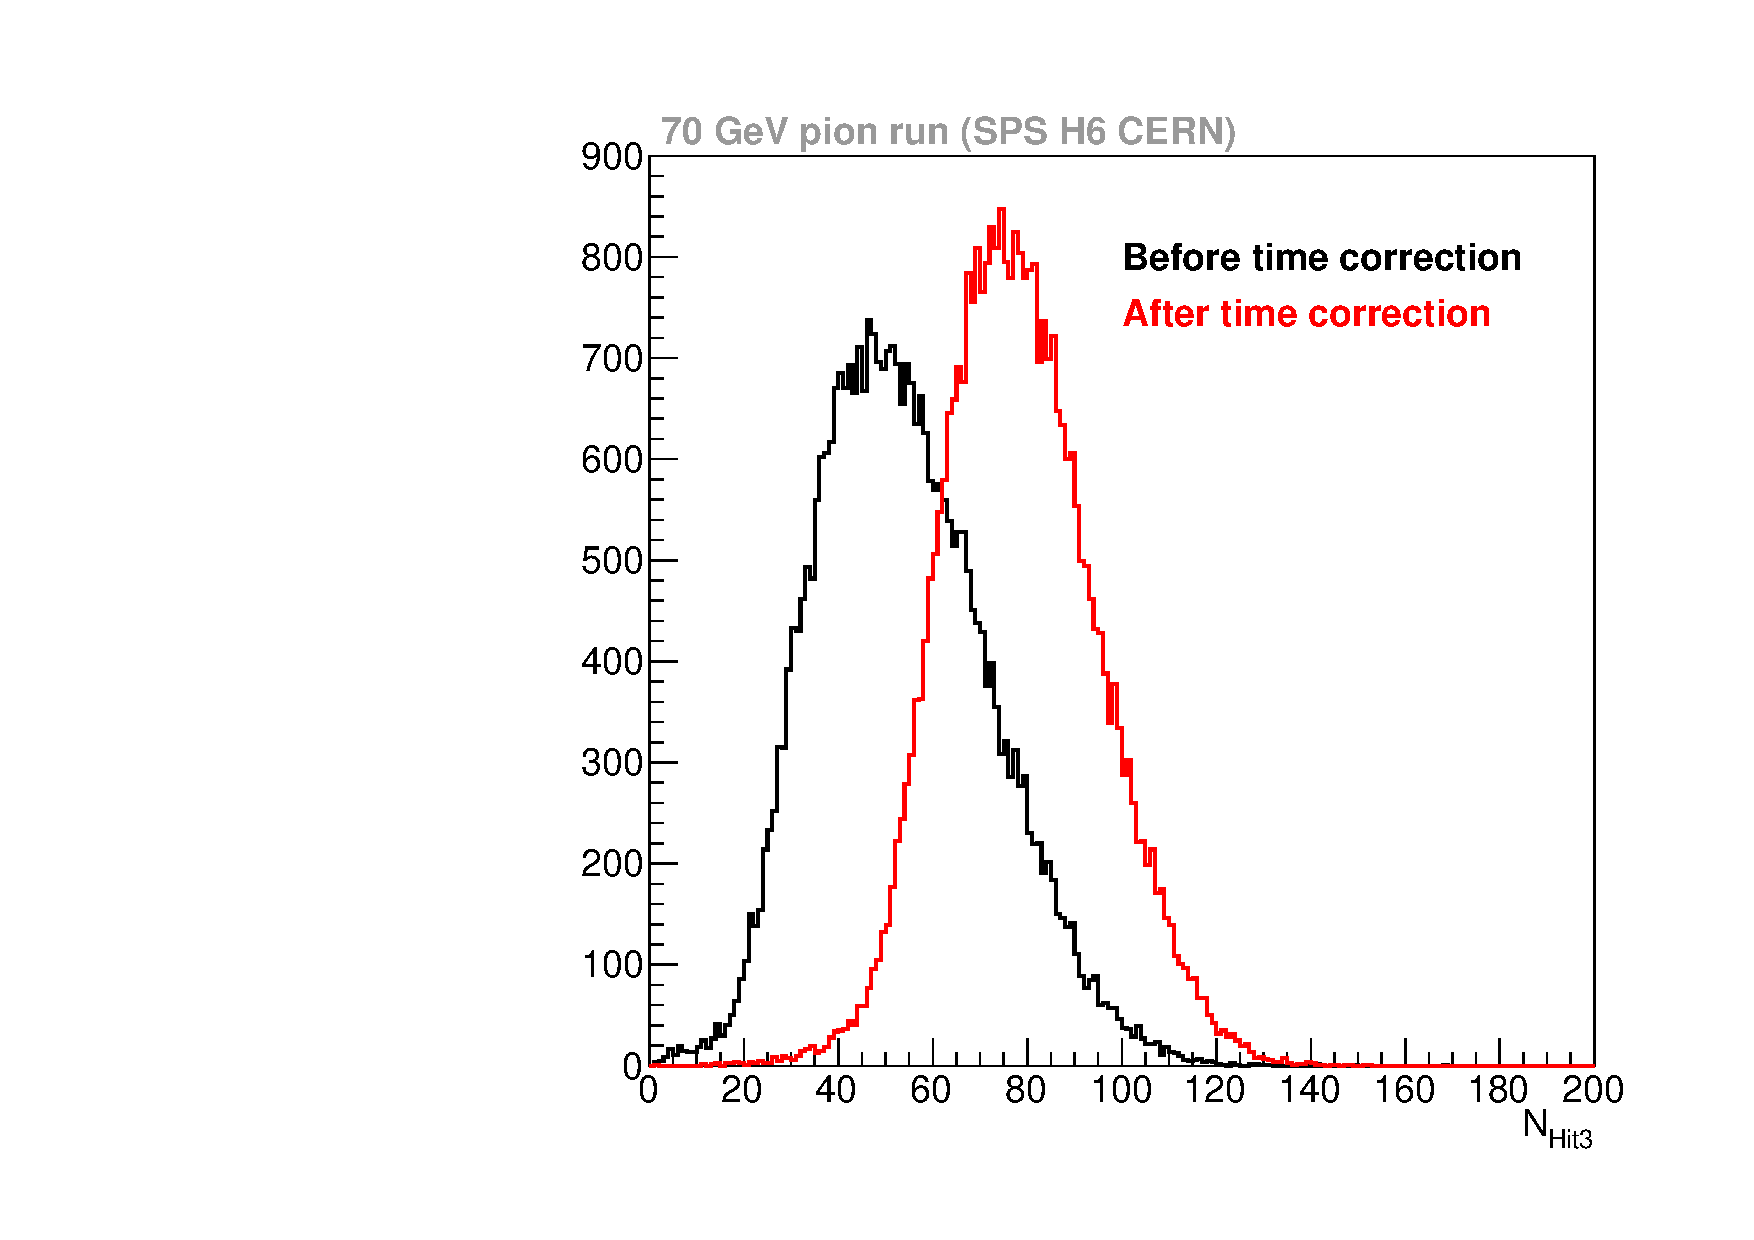
\includegraphics[width=.32\textwidth]{SDHCAL/figs/time_corr3.pdf}
    \caption{Distribution du nombre de hits pour les trois seuils à 70 $GeV$ avant (en noir) et après (en rouge) les corrections temporelles.}
    \label{fig:nhit_corrected}
  \end{center}
\end{figure}
La figure~\ref{fig:nhit_corrected} montre les distributions du nombre de hits pour les trois seuils à 70 $GeV$ avant et après les corrections temporelles. L'effet de ces corrections augmente logiquement avec le seuil. 
\begin{table}[!ht]
  \begin{center}
    \begin{tabular}{c|c|c}
      \rowcolor{black!20!white}$ $ & Avant correction & Après correction \\
      \rowcolor{black!5!white}\hline
      \rowcolor{black!5!white}$N_1$ & $832.3 \pm 0.78$ & $865.1 \pm 0.78$\\
      \rowcolor{black!5!white}$\sigma_{N1}$ & $142.8 \pm 0.55$ & $142.4 \pm 0.55$\\
      \rowcolor{black!5!white}$\frac{\sigma_{N1}}{N_1}$ & $0.172 \pm 0.001$& $0.165 \pm 0.001$\\
      \rowcolor{black!5!white}\hline
      \rowcolor{black!5!white}$N_2$ & $177.2 \pm 0.17$ & $197.7 \pm 0.17$\\
      \rowcolor{black!5!white}$\sigma_{N2}$ & $31.8 \pm 0.12$ & $31.1 \pm 0.18$\\
      \rowcolor{black!5!white}$\frac{\sigma_{N2}}{N_2}$ & $0.179 \pm 0.001$& $0.157 \pm 0.001$\\
      \rowcolor{black!5!white}\hline
      \rowcolor{black!5!white}$N_3$ & $53.2 \pm 0.10$ & $78.4 \pm 0.09$\\
      \rowcolor{black!5!white}$\sigma_{N3}$ & $18.4 \pm 0.07$ & $16.3 \pm 0.06$\\
      \rowcolor{black!5!white}$\frac{\sigma_{N3}}{N_3}$ & $0.346 \pm 0.002$& $0.208 \pm 0.001$\\
    \end{tabular}
  \end{center}  
  \caption{Nombre moyen de hits pour les trois seuils, écart type et résolution relative avant et après la correction temporelle.}
  \label{tab.n_comp}
\end{table}
Le tableau~\ref{tab.n_comp} présente les valeurs moyennes ($\bar N_i$), les écarts types ($\sigma_{Ni}$) et les résolutions ($\frac{\sigma_{Ni}}{N_i}$) des distributions de la figure~\ref{fig:nhit_corrected} pour chaque seuil $i$. Le nombre de hits augmente sensiblement après les corrections, alors que l'écart type et la résolution s'améliorent. 
Ces corrections nous permettront d'obtenir une meilleure résolution en énergie. Dans la suite de ce chapitre, les mentions au nombre de hits feront référence aux nombre de hits corrigés.

\subsection{Reconstruction de l'énergie des pions}
\label{sec.ereco}
Les procédures décrites dans les sections précédentes sont utilisées pour mesurer l’énergie des particules incidentes dans le prototype du SDHCAL. Rappelons que dans cette section, les corrections de gains ne sont pas appliquées: tous les canaux électroniques ont un gain fixé à 1. Les incertitudes systématiques présentes sur les différentes figures seront discutées à la fin de cette section.
\subsubsection{Réponse du SDHCAL aux gerbes hadroniques}
La première propriété des gerbes hadroniques extraite avec le prototype du SDHCAL est le nombre total de hits. La figure~\ref{fig:nhitLin} montre le nombre moyen de hits en fonction de l'énergie du hadron incident.
\begin{figure}[!ht]
  \begin{center}
    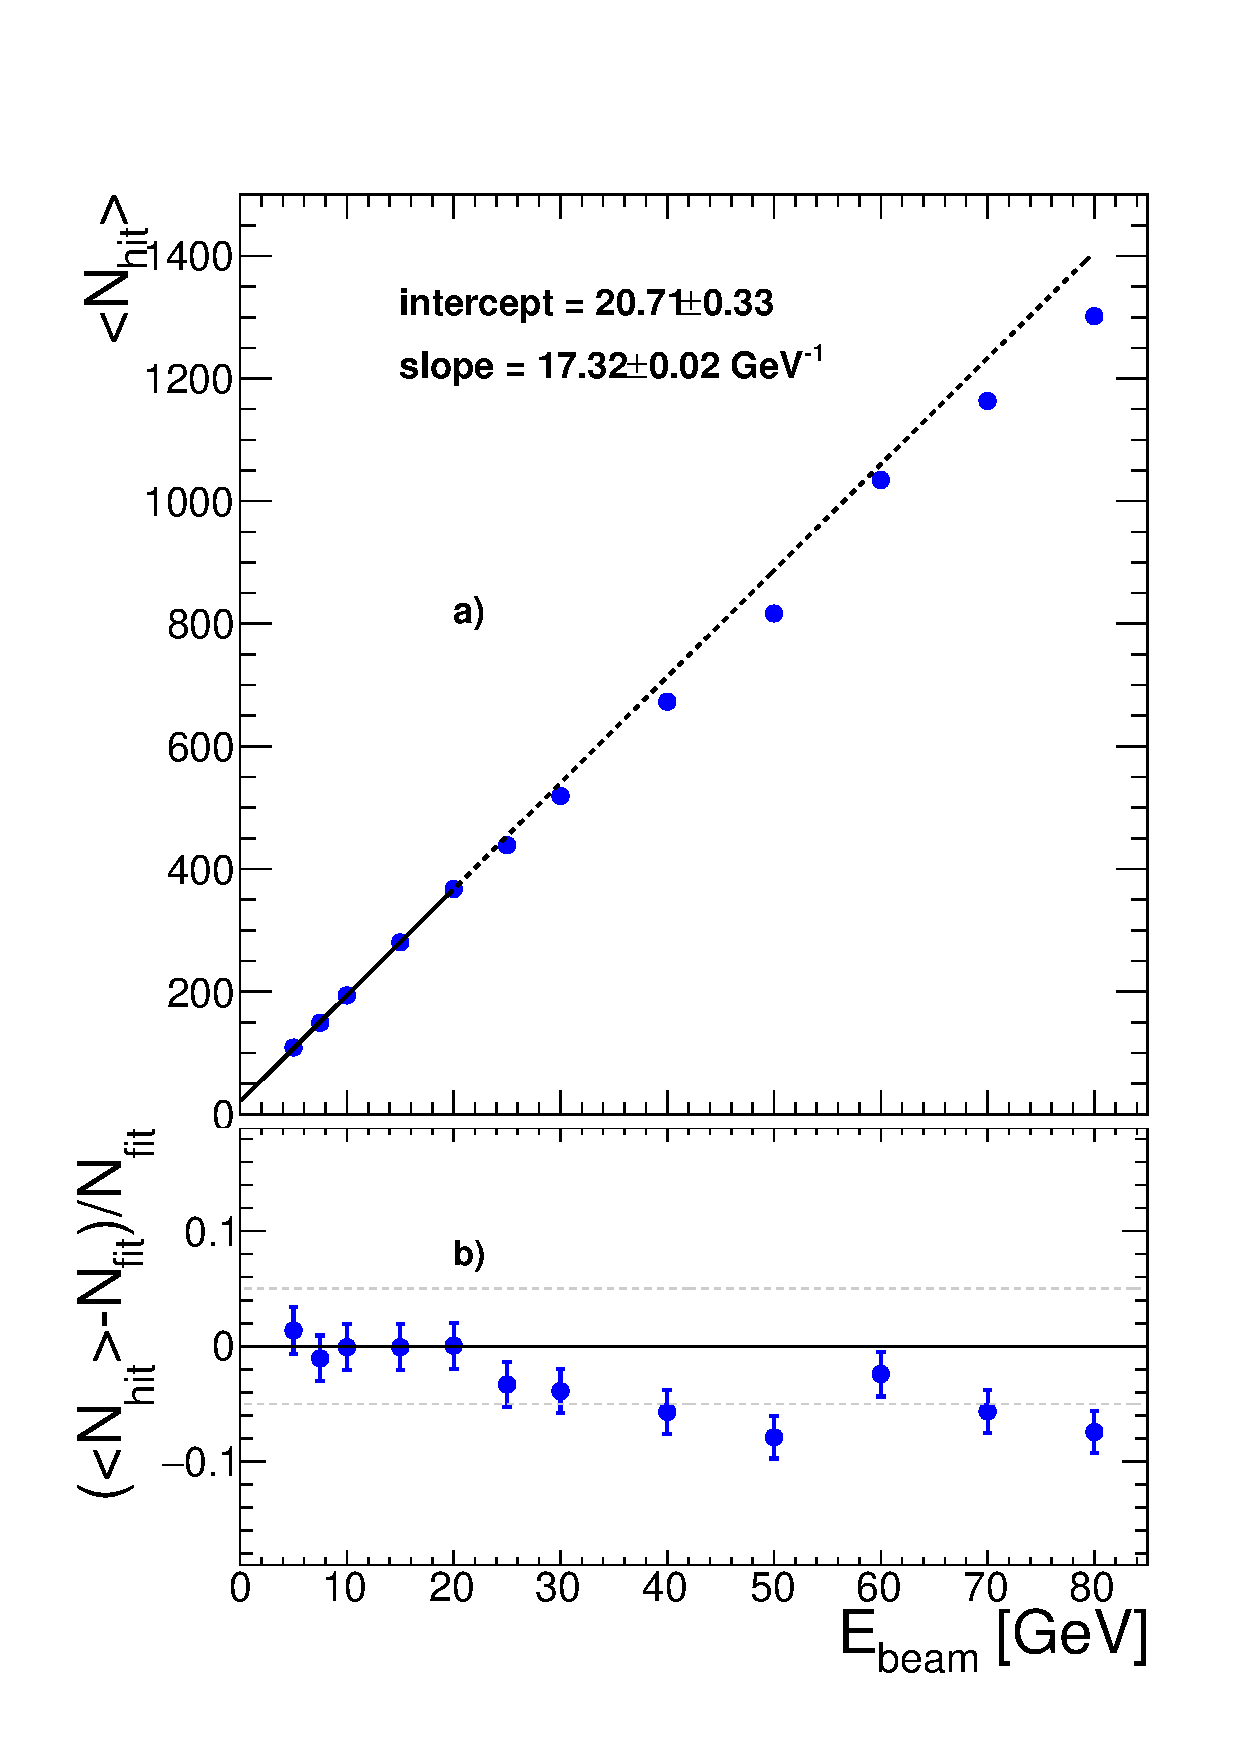
\includegraphics[width=.5\textwidth]{SDHCAL/figs/NHITPION.pdf}
    \caption{(a) Nombre moyen de hits en fonction de l'énergie du faisceau de la ligne H6 du CERN. La courbe noire pleine est un ajustement linéaire fait entre 5 et 20 $GeV$. La courbe noire en pointillé prolonge cet ajustement. (b) Déviation relative du nombre moyen de hits à l'ajustement linéaire en fonction de l'énergie du faisceau.}
    \label{fig:nhitLin}
  \end{center}
\end{figure}
Cette courbe est ajustée avec une fonction linéaire sur la gamme [5,20] $GeV$ (courbe noire trait plein). Cette courbe est prolongée sur toute la gamme d'énergie (courbe noire en pointillé). Cette figure présente aussi la déviation relative définie par $\frac{<N_{Hit}>-N_{Fit}}{N_{Fit}}$, où $<N_{Hit}>$ est le nombre moyen de hits et $N_{Fit}$ le nombre de hits attendus en utilisant le résultats de l'ajustement. Le nombre de hits dans le SDHCAL suit assez bien une fonction linéaire jusqu'à 20 $GeV$. Au delà de 25 $GeV$, on remarque que la réponse du SDHCAL sature avec l'énergie. A 60 $GeV$, le nombre de hits remonte brusquement. Ceci est probablement du à la contamination par les protons qui ont une longueur d'interaction plus faible que celle des pions. La fraction électromagnétique est aussi plus faible dans les cascades initiées par des protons que dans celles initiées par des pions.

\begin{figure}[!ht]
  \begin{center}
    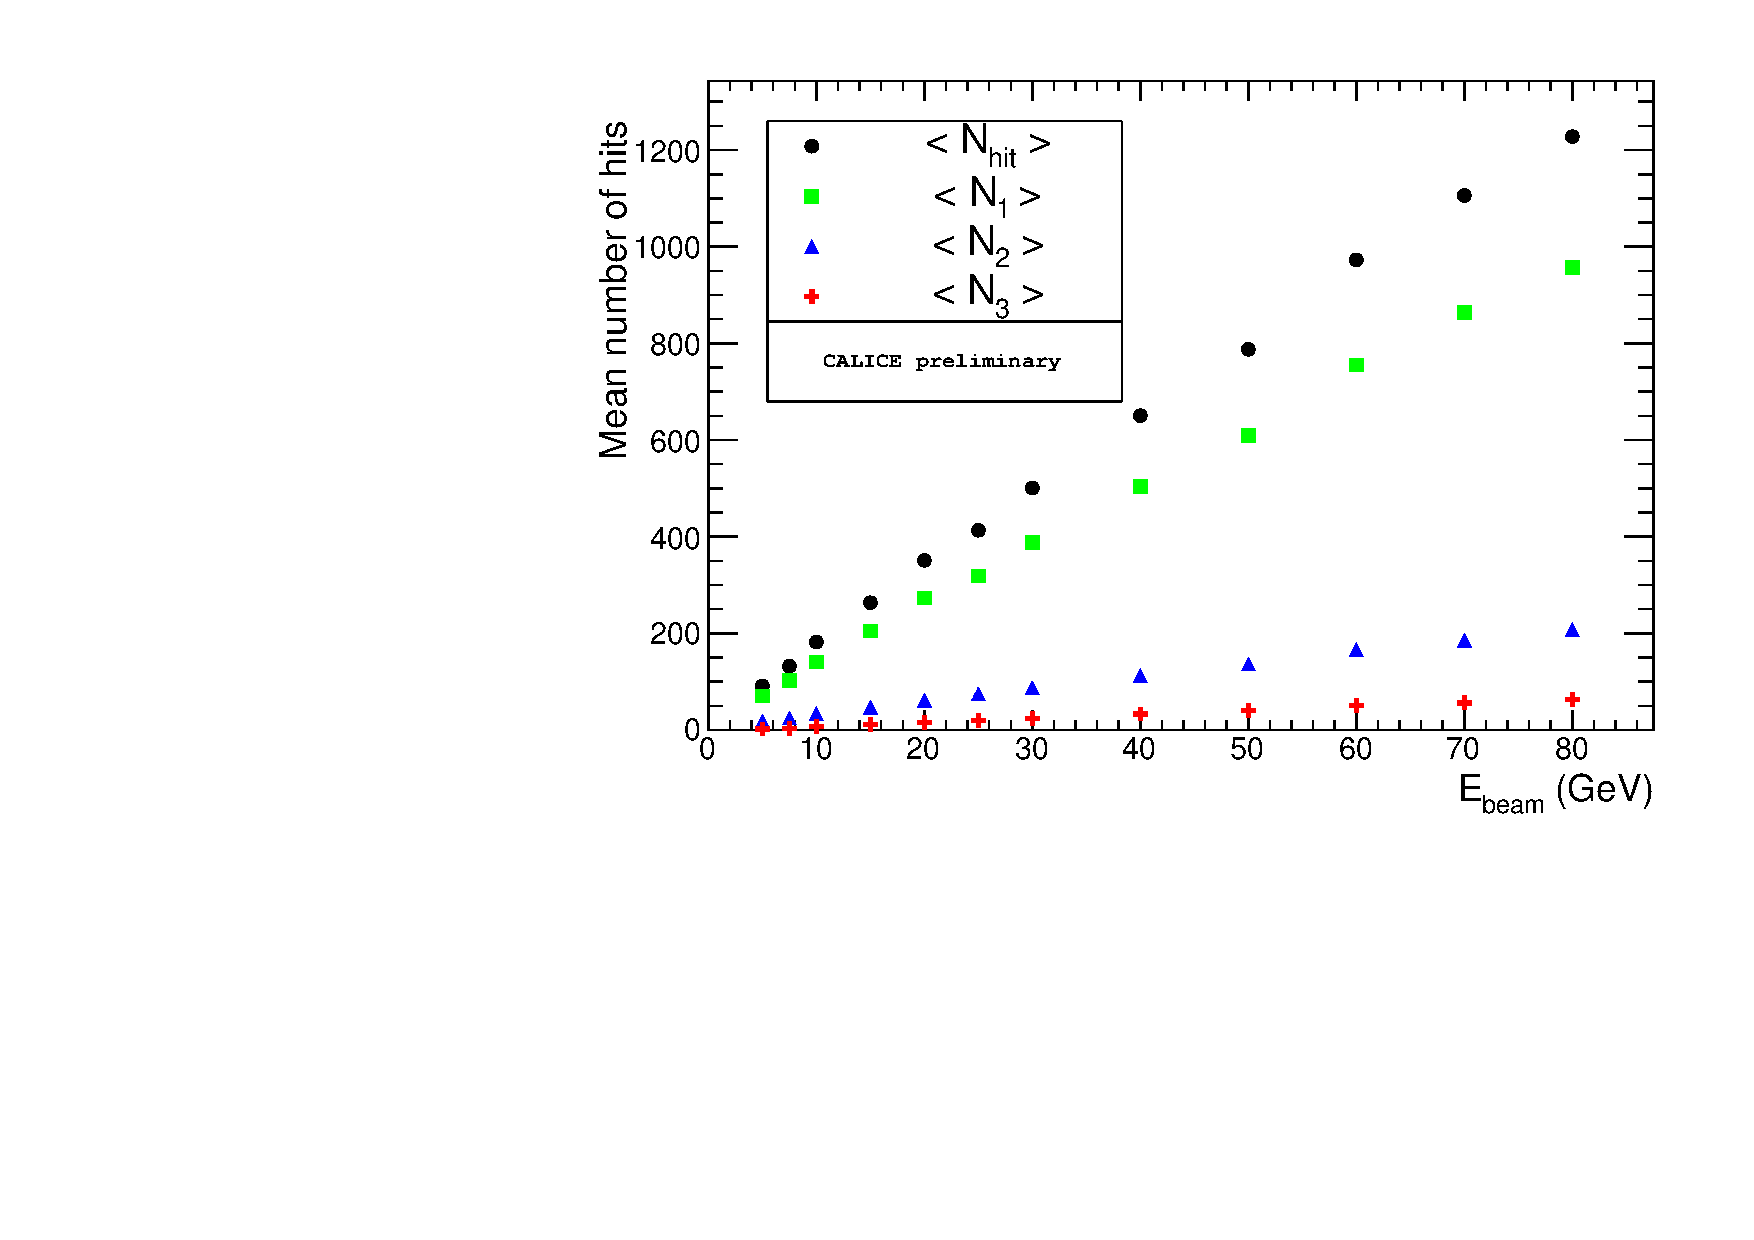
\includegraphics[width=.7\textwidth]{SDHCAL/figs/Nhit_N1_N2_N3.pdf}
    \caption{Nombre moyen de hits pour chaque seuil en fonction de l'énergie du faisceau. Les cercles noires représentent le nombre total de hits. Les carrés verts représentent le nombre de hits pour le seuil 1. Les triangles bleus représentent le nombre de hits pour le seuil 2. Les croix rouges représentent le nombre de hits pour le seuil 3.}
    \label{fig:nhit123}
  \end{center}
\end{figure}
La figure~\ref{fig:nhit123} présente le nombre moyen de hits pour chaque seuil, en fonction de l'énergie des hadrons incidents. L'utilisation des seuils permettra de corriger l'effet de la saturation vue sur la figure~\ref{fig:nhitLin} afin d'améliorer la résolution en énergie.

\subsubsection{Le mode binaire}
Une première méthode pour reconstruire l'énergie des particules incidentes utilise uniquement le nombre de hits de chaque événement. L'énergie est mesurée grâce à l'équation suivante:
\begin{equation}
  E_{reco} = A \cdot N_{Hit}
\end{equation}
où $A$ est une constante déterminée avec les données expérimentales. Cependant, la saturation observée sur la figure~\ref{fig:nhitLin} ne permet pas d'obtenir une linéarité satisfaisante au dessus de 30 $GeV$. Pour restaurer la linéarité, plusieurs paramétrages ont été testés. Le paramétrage suivant permet d'obtenir une linéarité raisonnable:
\begin{equation}
  \label{eq.ereco_bin}
  E_{reco} = A \cdot N_{Hit} + B \cdot N_{Hit}^2 + C \cdot N_{Hit}^3
\end{equation}
Les constantes $A$, $B$ et $C$ sont déterminées avec les données expérimentales en minimisant le $\chi^2$ suivant:
\begin{equation}
  \chi^2 = \frac{\sum_{i=0}^{N_{events}}(E_{inc}^i-E_{reco}^i)^2}{E_{inc}^i}
\end{equation}
où $N_{events}$ est le nombre d'événements utilisés pour la minimisation et $E_{inc}^i$ est l'énergie de la particule incidente $i$. La figure~\ref{fig:energy_dist_bin} montre deux distributions d'énergie reconstruite pour des échantillons de données à 20 et 40 $GeV$. 
\begin{figure}[!ht]
  \begin{center}
    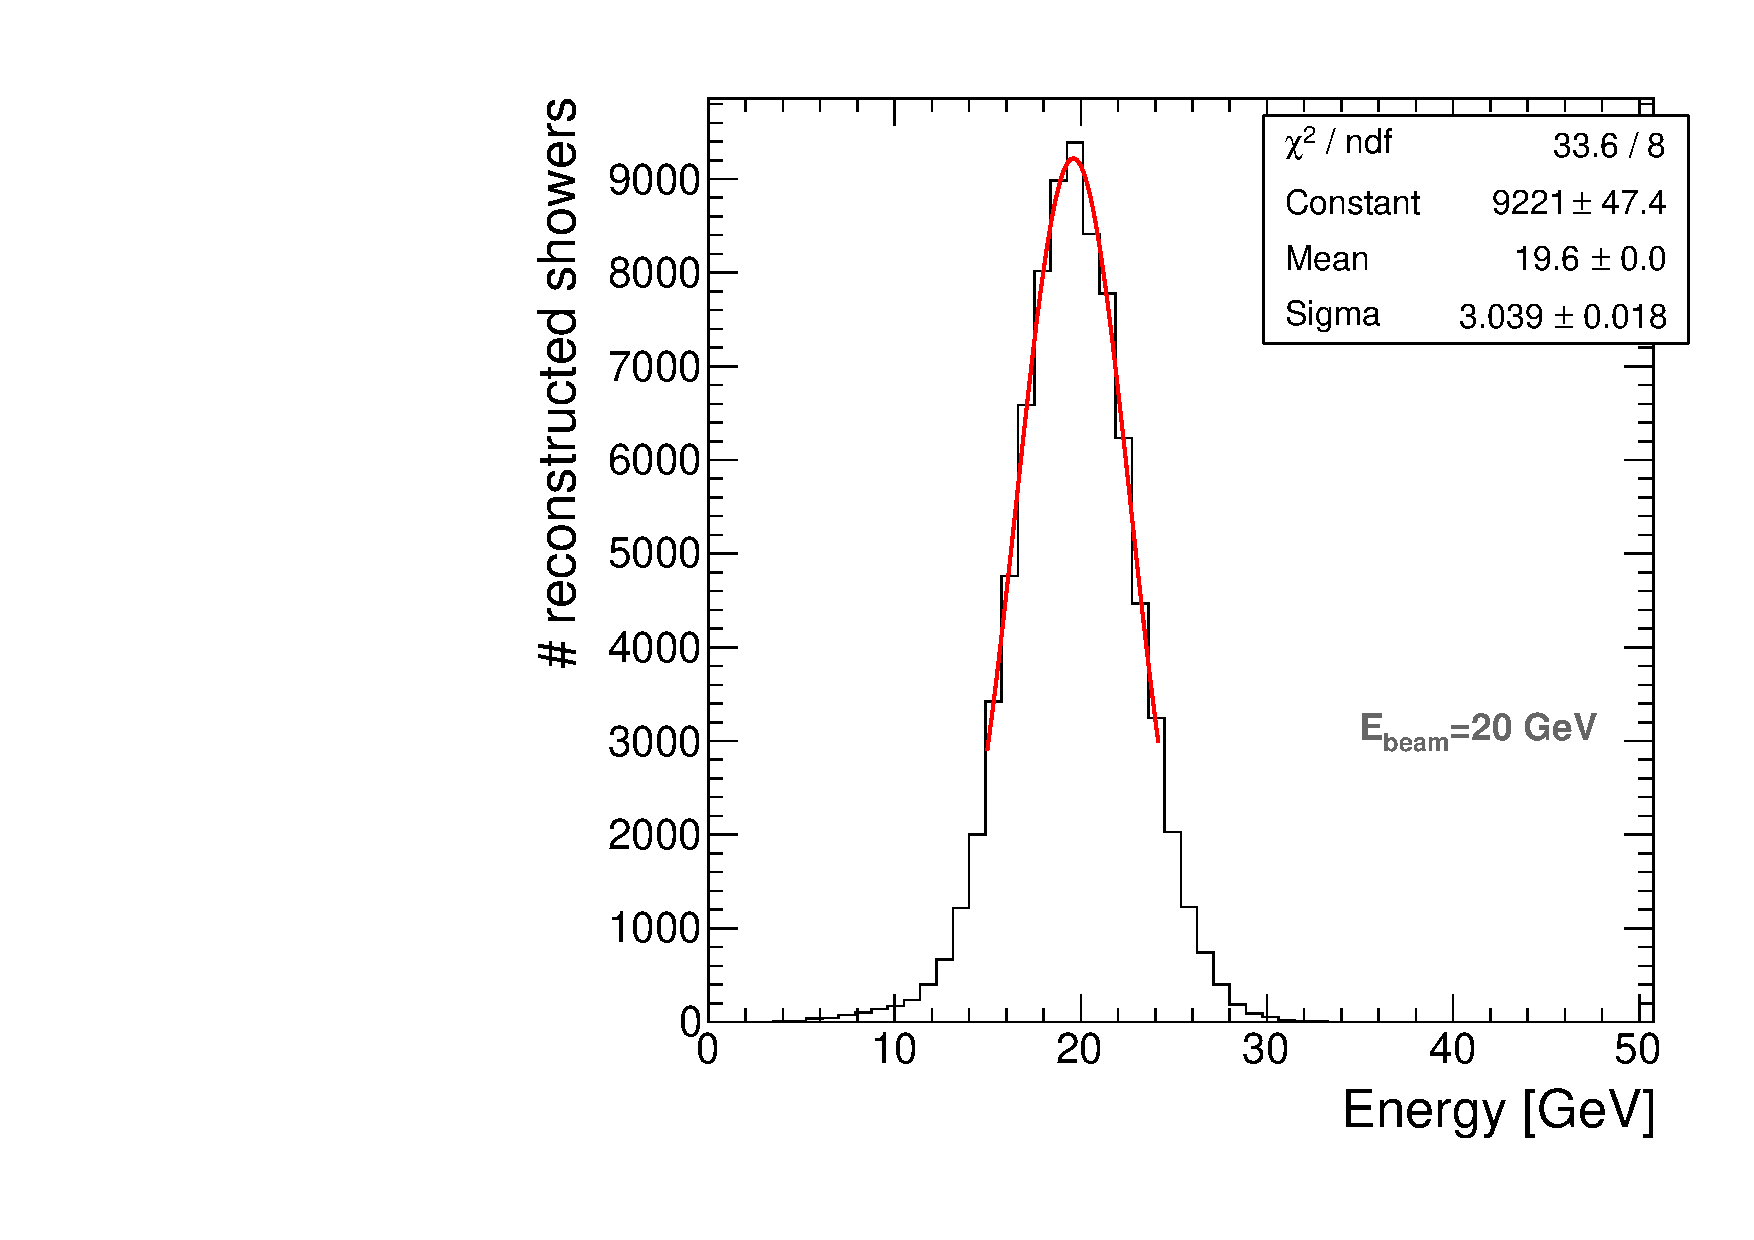
\includegraphics[width=.45\textwidth]{SDHCAL/figs/gfit-en-20-bin.pdf}
    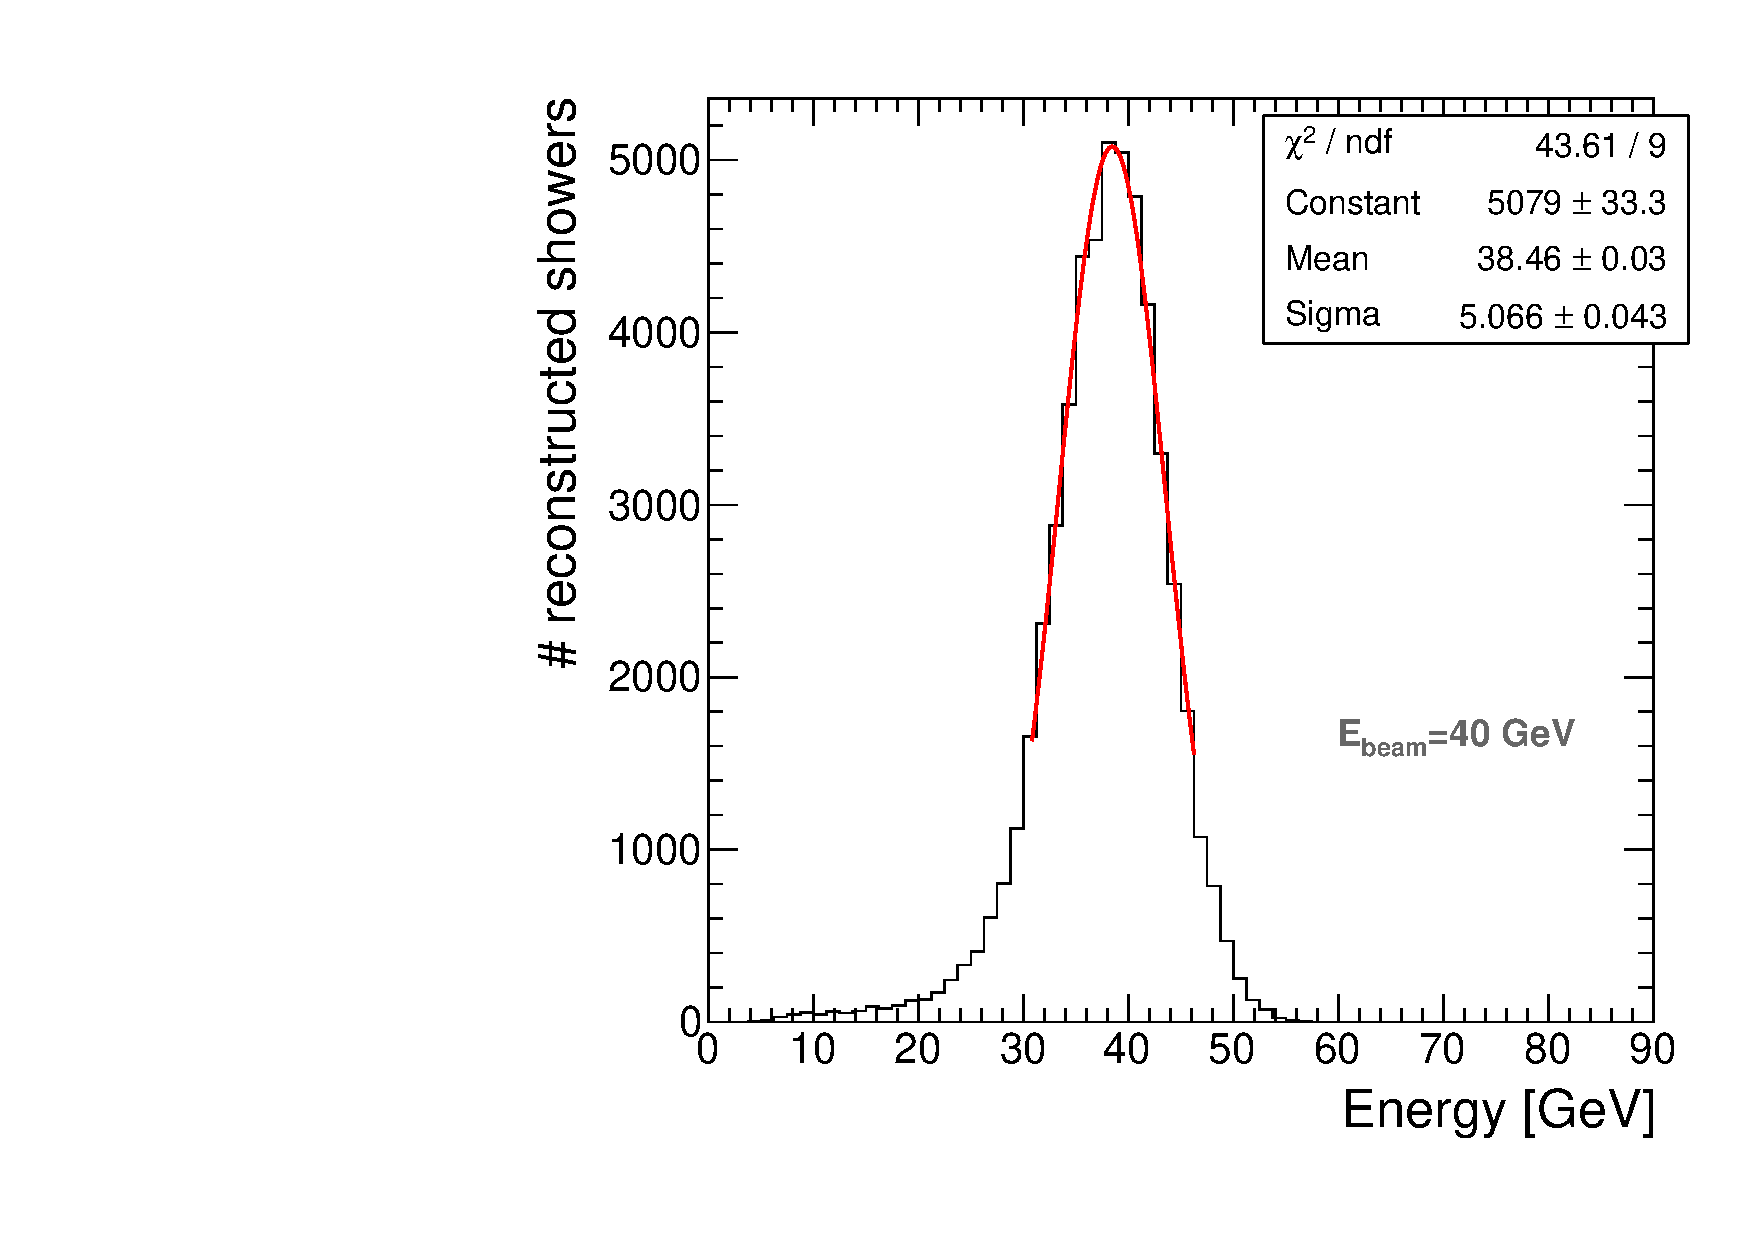
\includegraphics[width=.45\textwidth]{SDHCAL/figs/gfit-en-40-bin.pdf}
    \caption{Distribution en énergie des gerbes hadroniques reconstruites. L'énergie est calculée avec le mode binaire sans l'information des seuils. Les distributions sont ajustées avec des gaussiennes dans une gamme de $\pm1.5\sigma$ autour de la valeur moyenne.}
    \label{fig:energy_dist_bin}
  \end{center}
\end{figure}
Les distributions d'énergie sont ajustées en deux temps, avec une fonction gaussienne. La valeur moyenne $\bar{E}_{reco}$ et le $\sigma$ d'un premier ajustement définissent la gamme [$\bar{E}_{reco}-1.5\sigma$ , $\bar{E}_{reco}+1.5\sigma$] pour le second ajustement. Cette méthode d'ajustement permet de s'affranchir des queues de distribution à basse énergie (à gauche sur les distributions en énergie). Ces queues de distribution sont dues aux hadrons qui interagissent tardivement dans le détecteur. Ainsi, une fraction importante de l'énergie incidente n'est pas déposée dans le détecteur ce qui détériore la reconstruction de l'énergie. La figure~\ref{fig:energy_bin}(a) montre l'énergie reconstruite moyenne et la déviation relative en fonction de l'énergie du faisceau. La déviation relative est définie par $\frac{E_{reco}-E_{beam}}{E_{beam}}$ ($E_{beam}$ est l'énergie du faisceau). Cette figure montre une très bonne linéarité ($\frac{E_{reco}-E_{beam}}{E_{beam}}<5\%$ sur toute la gamme d'énergie sauf à 5 $GeV$), ce qui valide le choix du paramétrage de $E_{reco}$. La figure~\ref{fig:energy_bin}(b) montre la résolution relative en fonction de l'énergie du faisceau.
\begin{figure}[!ht]
  \begin{center}
    \subfigure[]{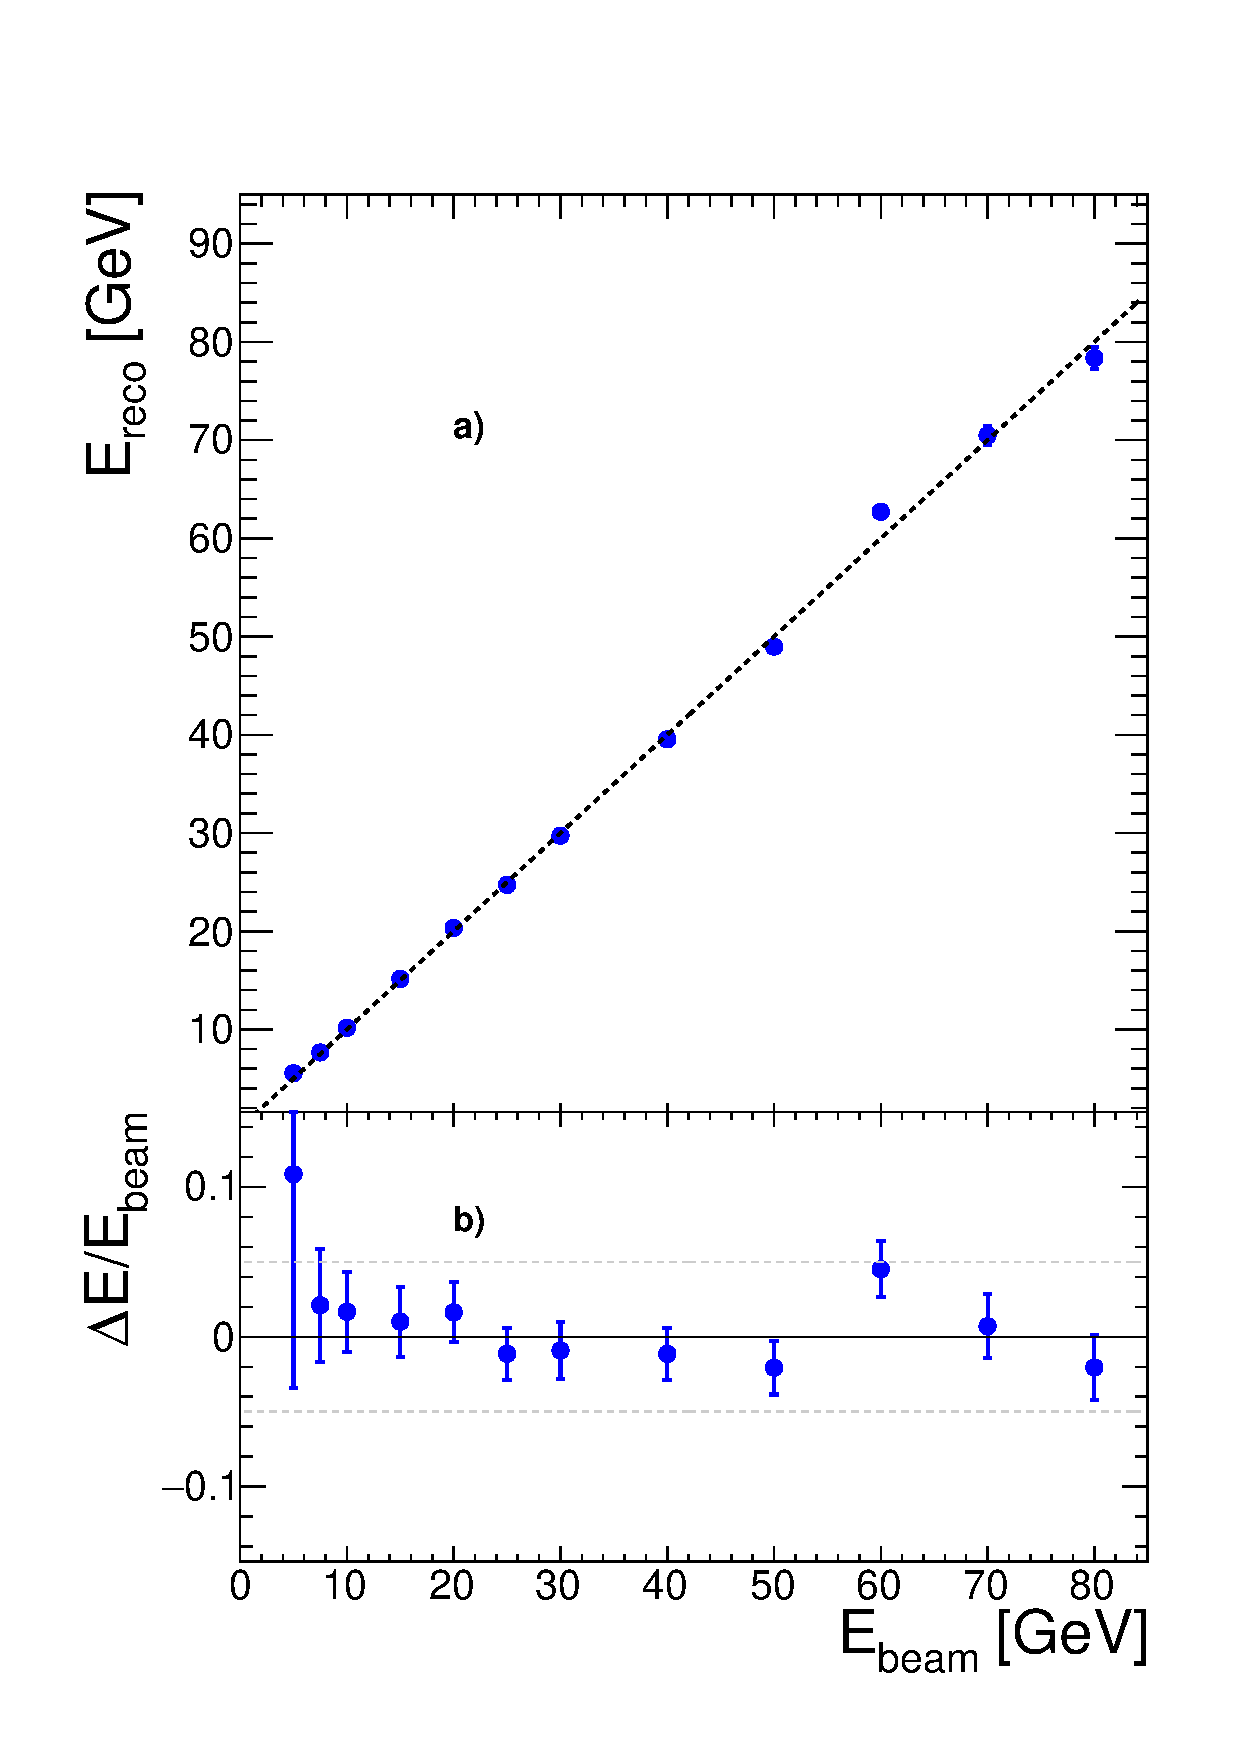
\includegraphics[width=.44\textwidth]{SDHCAL/figs/LINEARITY_bin_10.pdf}}
    \subfigure[]{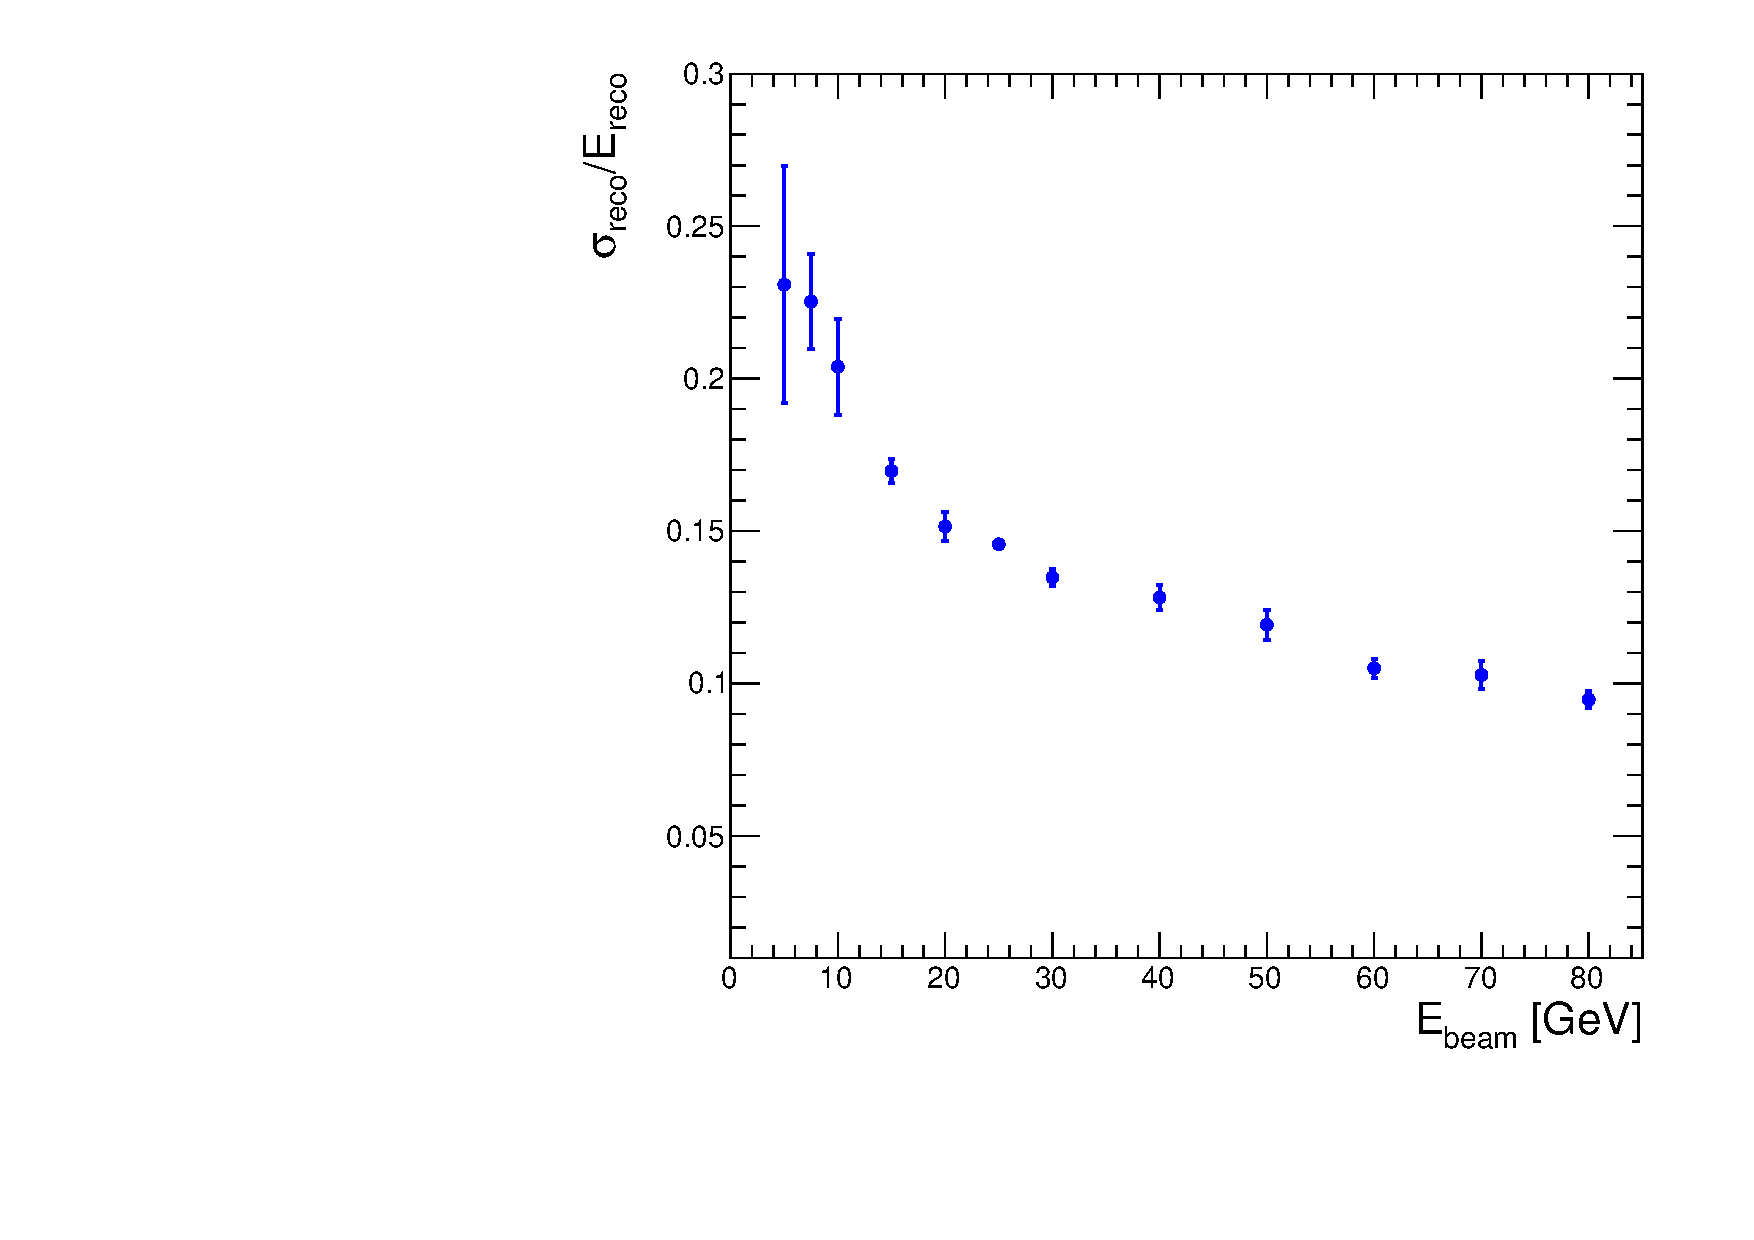
\includegraphics[width=.55\textwidth]{SDHCAL/figs/RESO_bin_10.pdf}}
    \caption{(a): Énergie reconstruite moyenne des gerbes hadroniques et déviation relative en fonction de l'énergie du faisceau (ligne~H6). (b): Résolution relative ($\frac{\sigma_{reco}}{E_{reco}}$) de l'énergie reconstruite en fonction de l'énergie du faisceau (ligne~H6). L'énergie est calculée en utilisant uniquement le nombre total de hits (équation~\ref{eq.ereco_bin}).}
    \label{fig:energy_bin}
  \end{center}
\end{figure}

\subsubsection{Le mode multi-seuils}
La spécificité du SDHCAL est son mode de lecture semi-digitale. Comme nous l'avons déjà expliqué, le seuil déclenché permet d'avoir une idée du nombre de particules secondaires traversant la couche de gaz vers un canal de lecture. Les informations sur les seuils devraient aider à combattre le phénomène de saturation vu sur la figure~\ref{fig:nhitLin} et à améliorer la résolution en énergie. Les informations des seuils pourraient aussi aider à comprendre la structure des gerbes hadroniques en identifiant les zones denses en particules secondaires. Une première tentative pour calculer l'énergie reconstruite des gerbes hadroniques utilisait l'équation suivante:
\begin{equation}
  E_{reco}=\alpha\cdot N1+\beta\cdot N2+\gamma\cdot N3
  \label{eq.erec}
\end{equation}
avec $N1$, $N2$ et$N3$ les nombres de hits relatifs à chaque seuil. Les constantes $\alpha$, $\beta$ et $\gamma$ sont déterminées avec les données. Cependant, il s'est avéré impossible de trouver un paramétrage de ces constantes donnant une bonne linéarité et une bonne résolution en énergie. Ainsi, comme pour le mode binaire, les paramètres de reconstruction de l'énergie sont des fonctions du nombre total de hits, ce qui permet de tenir compte de l'énergie. Le meilleur paramétrage obtenue est une fonction quadratique du nombre de hits (exemple:~$\alpha~=~A_1+B_1\cdot N_{Hit}+C_1\cdot N_{Hit}^2$). De même que pour le mode binaire, les valeurs des paramètres de l'énergie reconstruite sont déterminées avec une méthode de minimisation d'un $\chi^2$. Les données obtenues sur la ligne H2 sont utilisées pour estimer les paramètres de l'énergie reconstruite. Ces paramètres sont ensuite utilisés pour calculer l'énergie des hadrons des lignes H2 et H6.
\begin{figure}[!ht]
  \begin{center}
    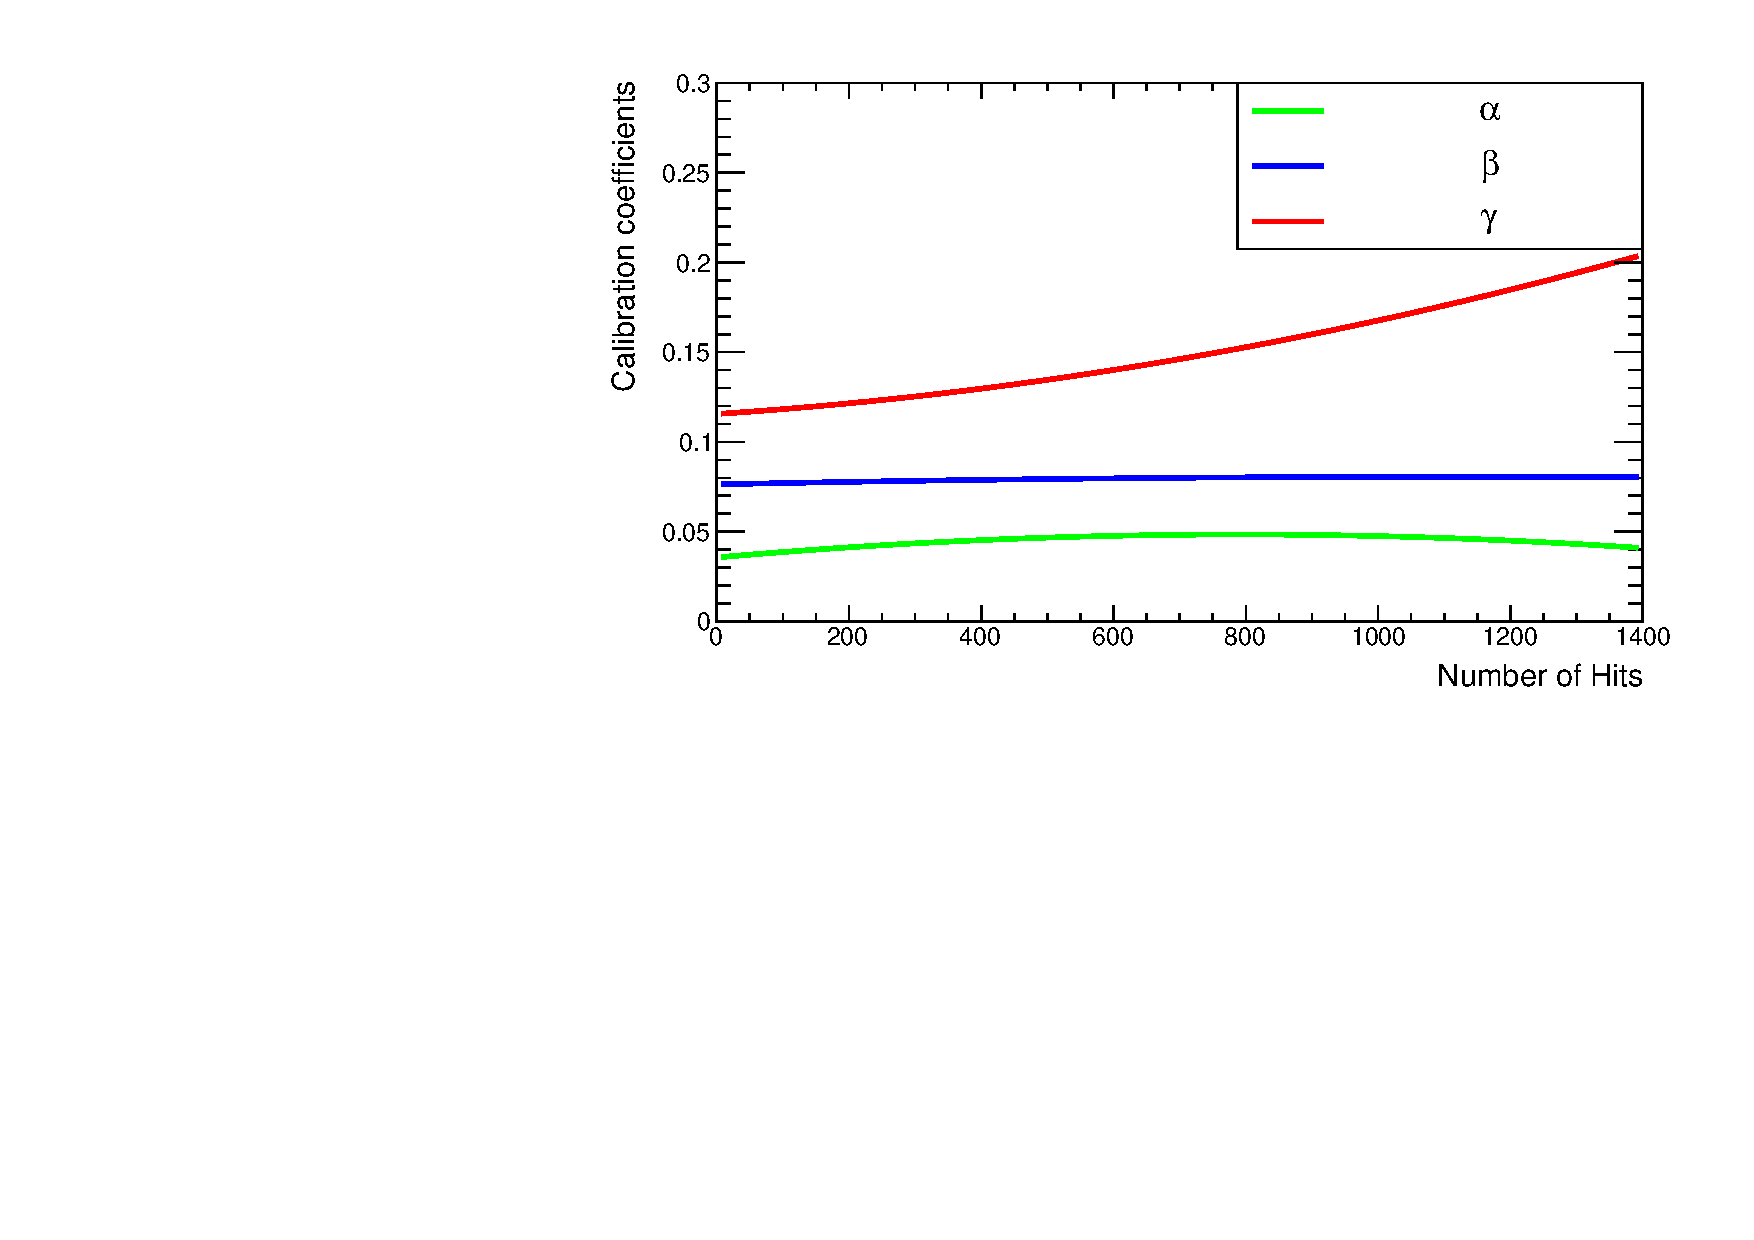
\includegraphics[width=.7\textwidth]{SDHCAL/figs/evolution.pdf}
    \caption{Évolution des paramètres de reconstruction de l'énergie en fonction du nombre total de hits. L'énergie est reconstruite en utilisant l'information des seuils.}
    \label{fig:evol}
  \end{center}
\end{figure}
\begin{figure}[!ht]
  \begin{center}
    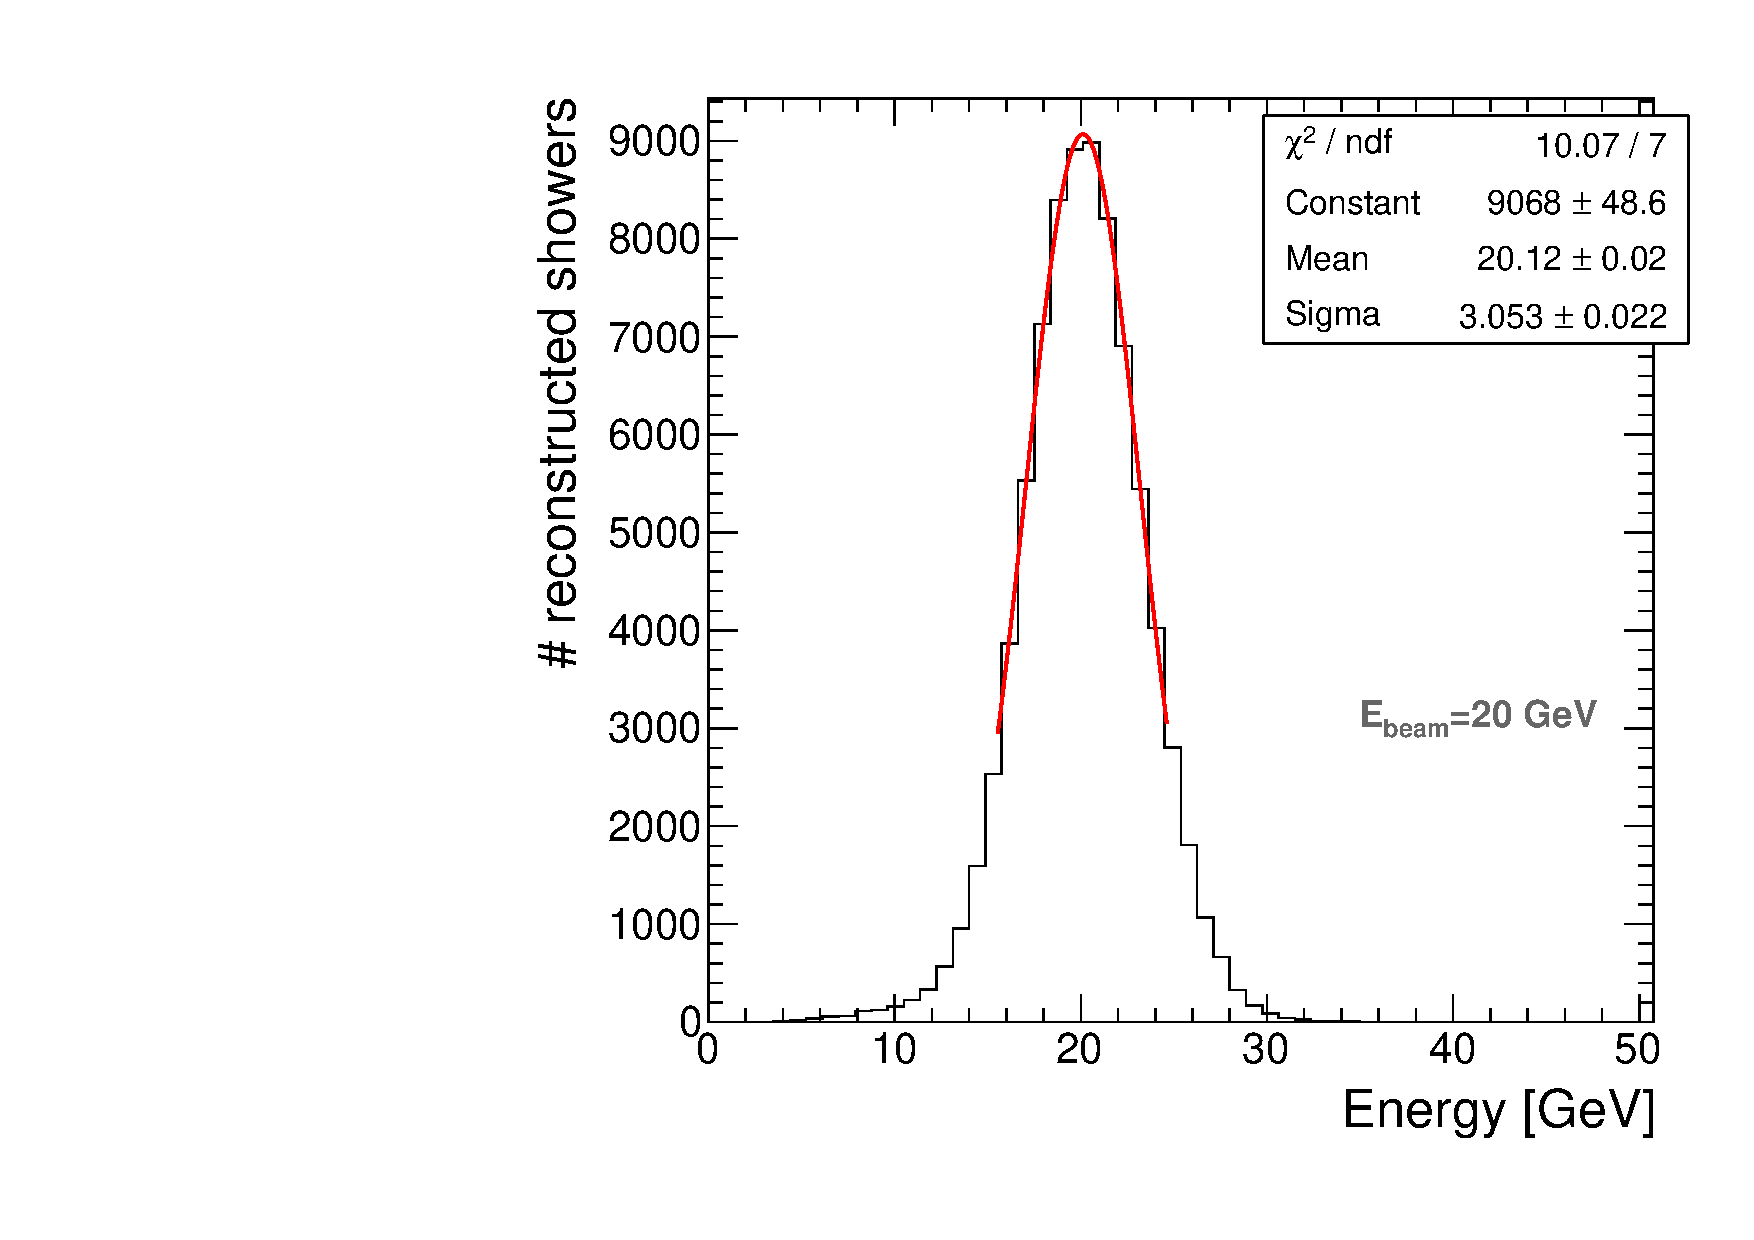
\includegraphics[width=.45\textwidth]{SDHCAL/figs/gfit-en-20.pdf}
    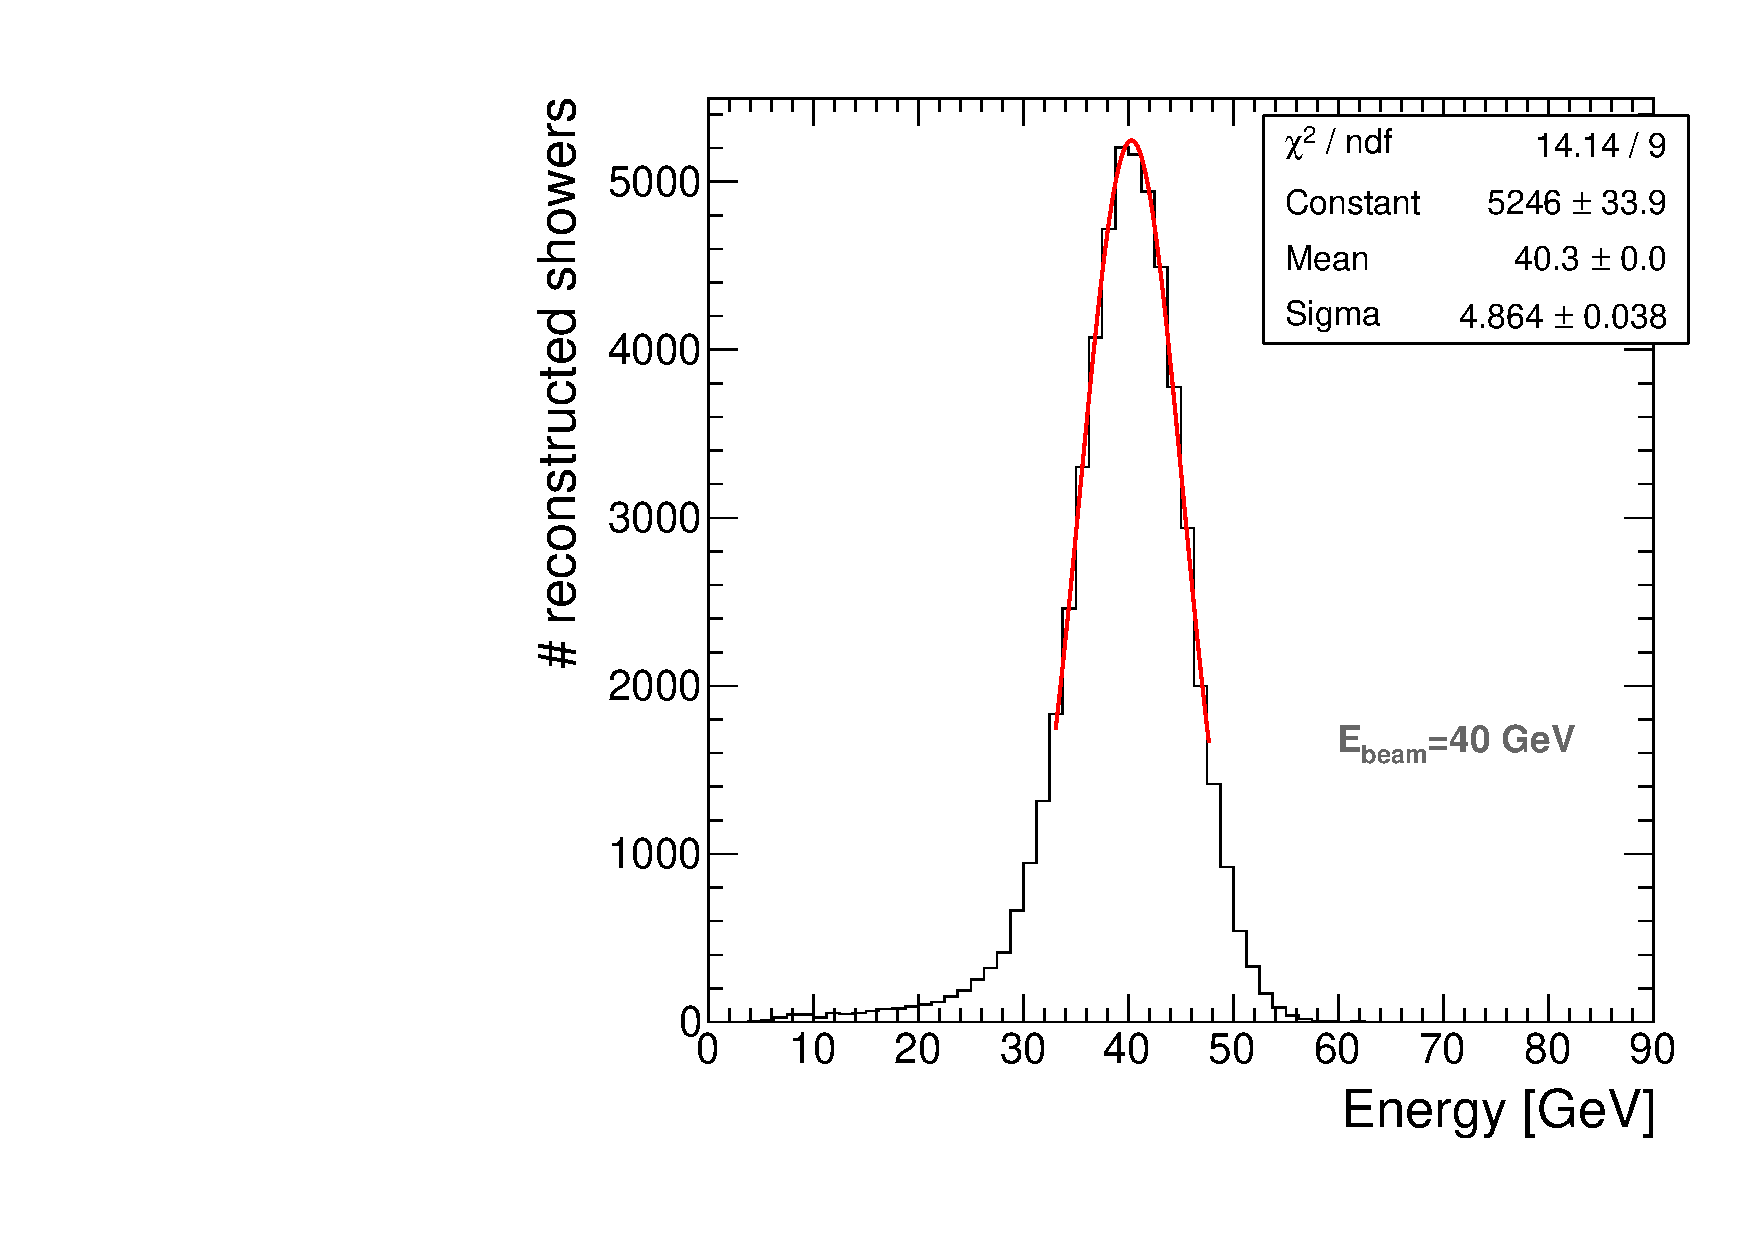
\includegraphics[width=.45\textwidth]{SDHCAL/figs/gfit-en-40.pdf}
    \caption{Distribution de l'énergie reconstruite pour des échantillons de gerbes hadroniques à 20 et 40 $GeV$.}%L'énergie est calculée avec le mode multi-seuils. Les distributions sont ajustées avec des gaussiennes dans une gamme de $\pm1.5\sigma$ autour de la valeur moyenne.}
    \label{fig:energy_dist_sd}
  \end{center}
\end{figure}
La figure~\ref{fig:evol} montre l'évolution des paramètres de reconstruction de l'énergie en fonction du nombre total de hits. Le coefficient $\gamma$ (pour le troisième seuil) augmente avec le nombre de hits. Cela confirme l'idée que la présence des seuils aide à traiter le phénomène de saturation. 
La figure~\ref{fig:energy_dist_sd} montre deux distributions d'énergie reconstruite à 20 et 40 $GeV$ en utilisant la méthode multi-seuils. De même que pour le mode binaire, les distributions d'énergie reconstruite sont ajustées en deux étapes avec une fonction gaussienne. 
\begin{figure}[!ht]
  \begin{center}
    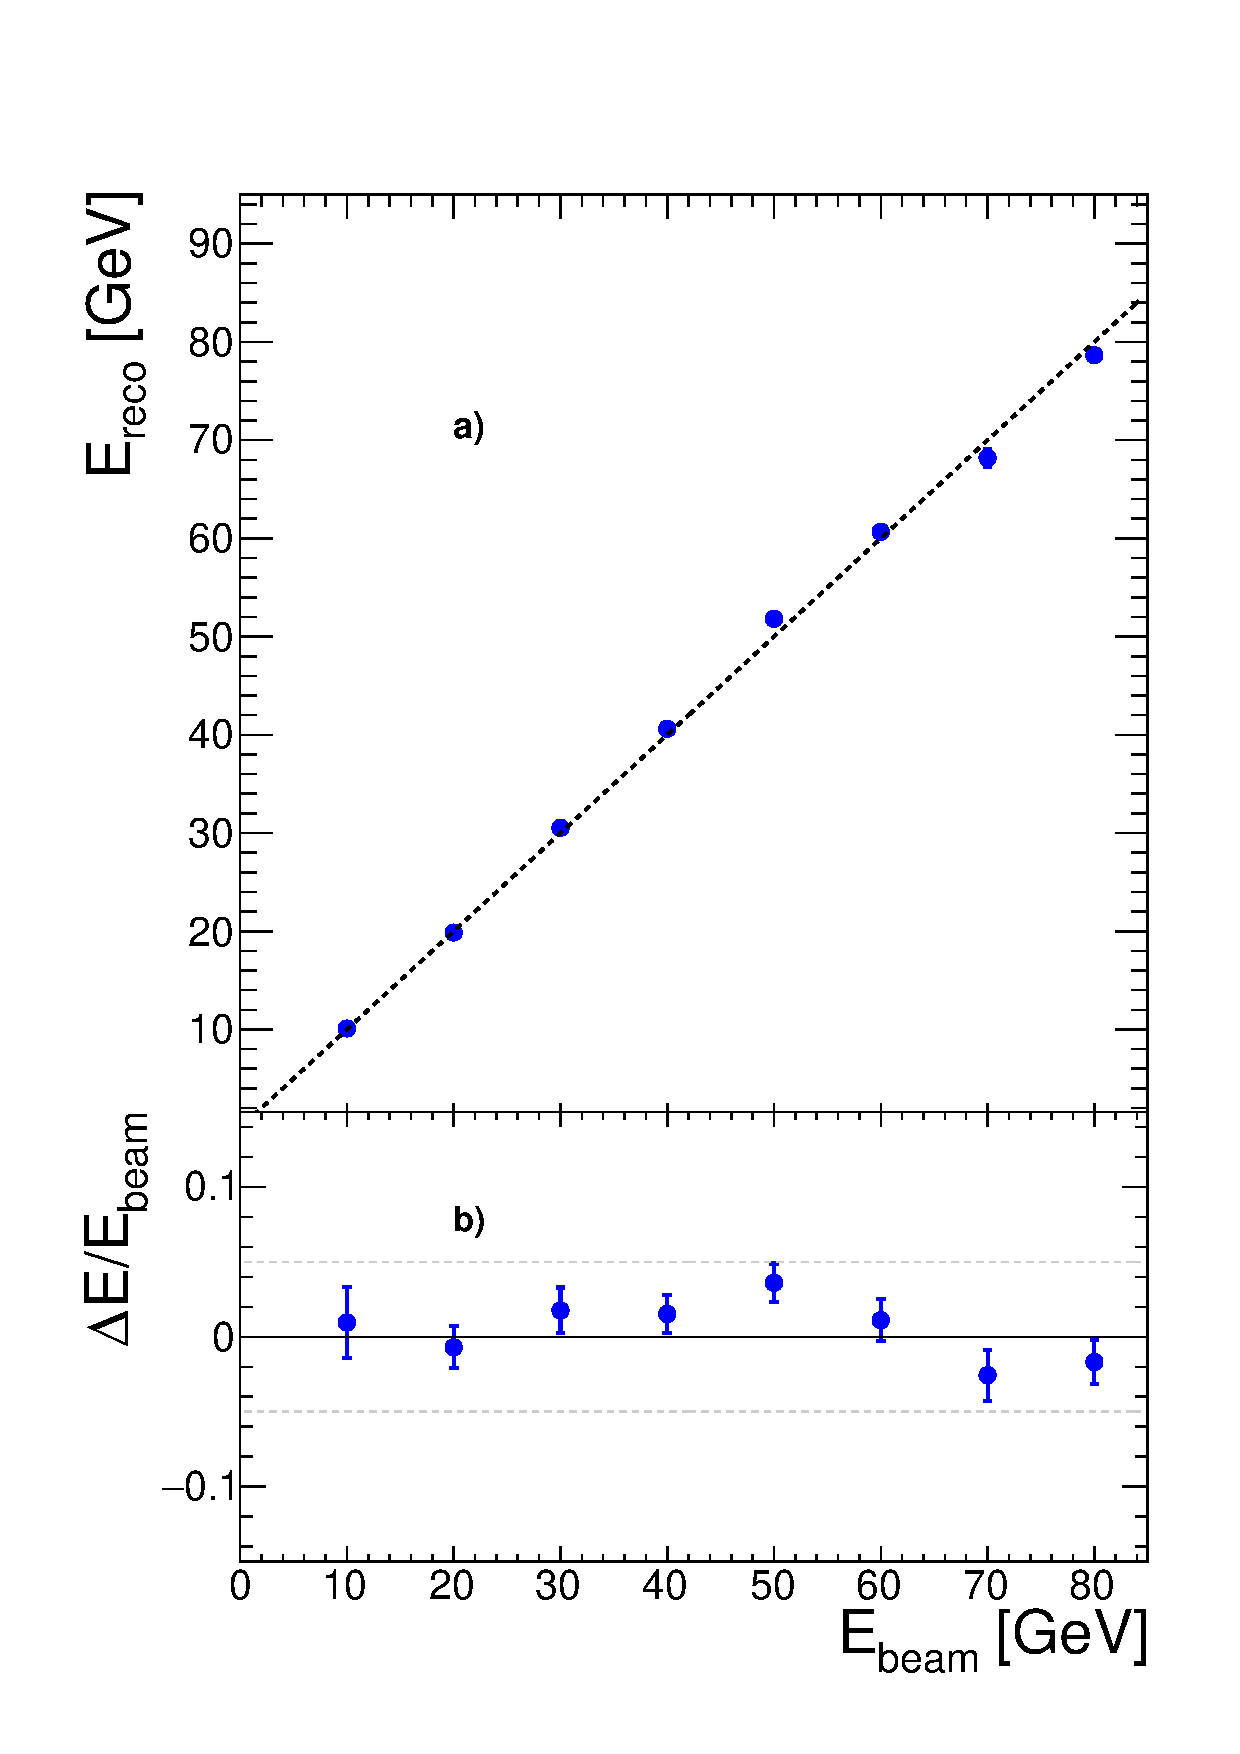
\includegraphics[width=.49\textwidth]{SDHCAL/figs/LINEARITY_Nov_10.pdf}
    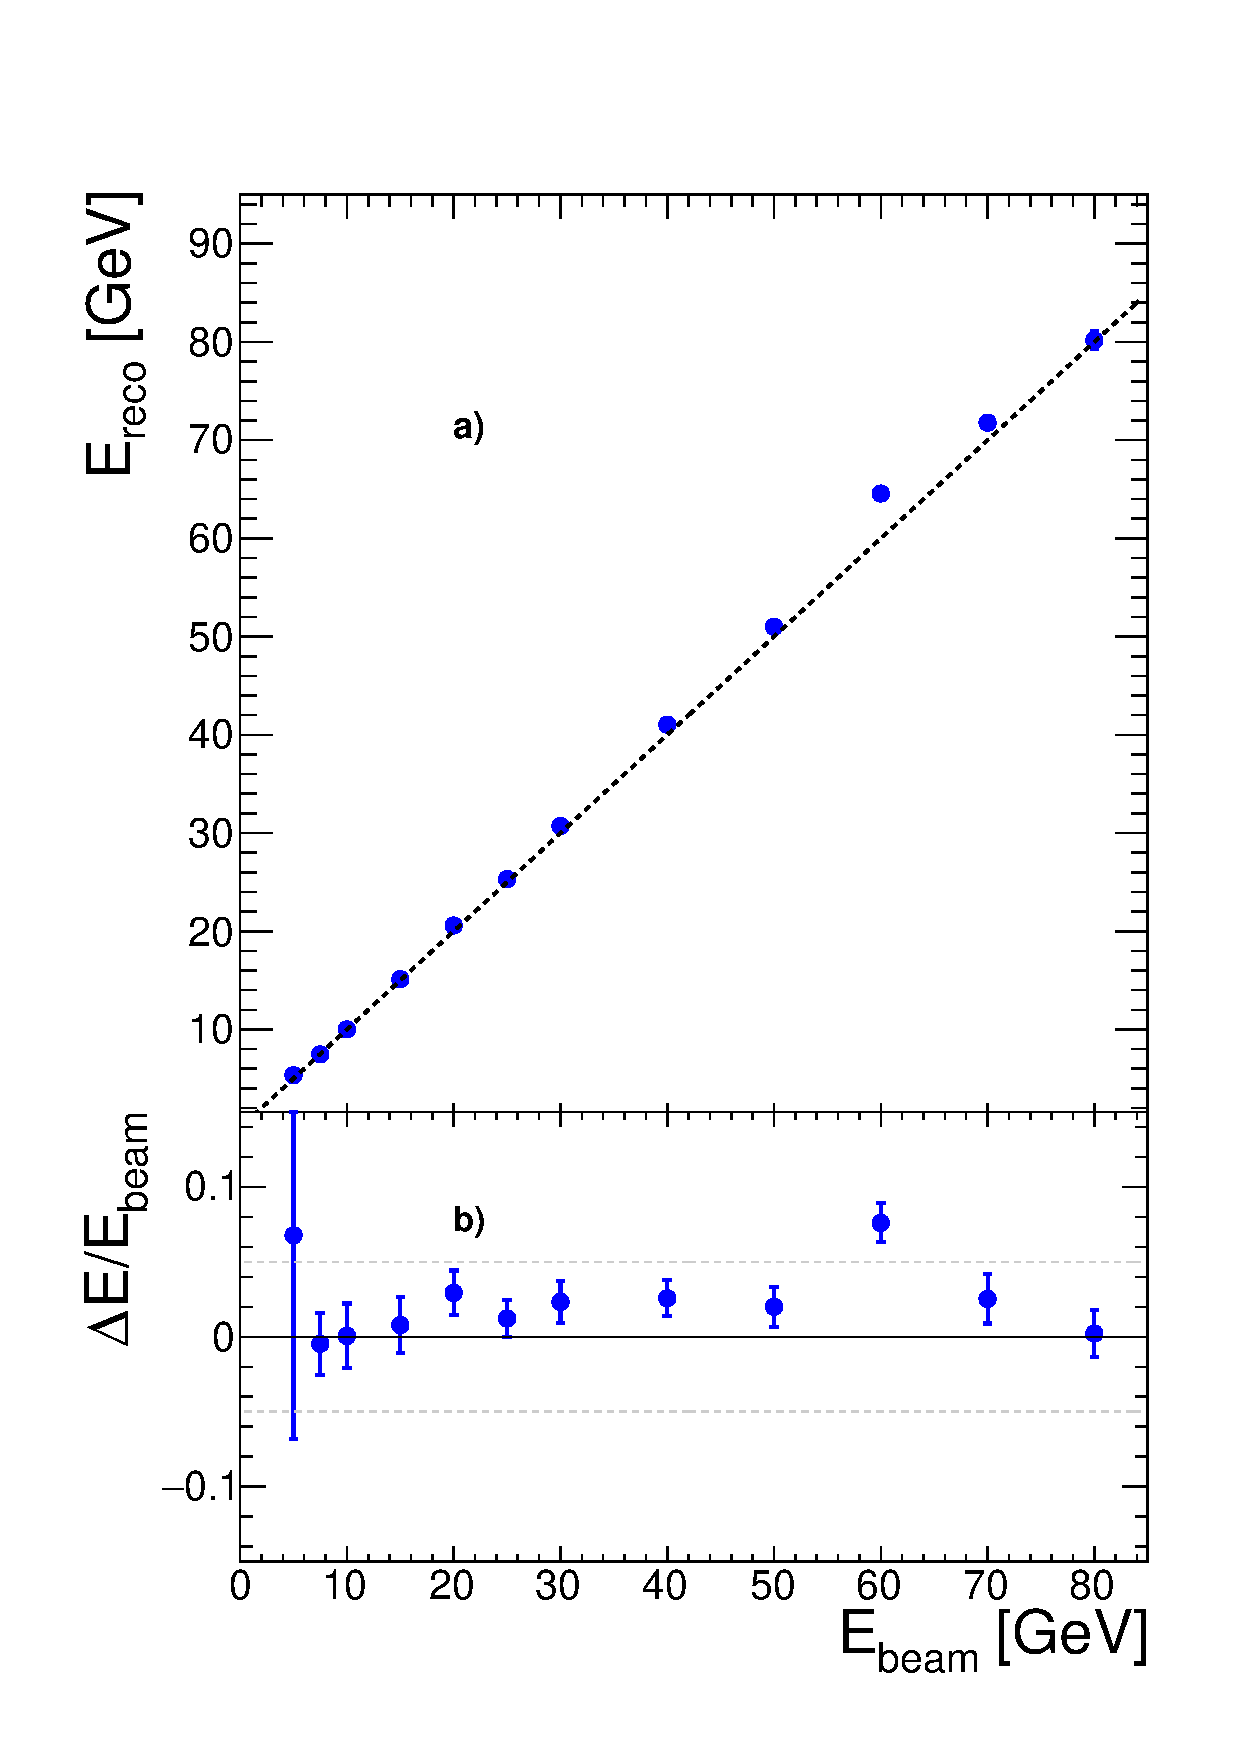
\includegraphics[width=.49\textwidth]{SDHCAL/figs/LINEARITY_Sept_10.pdf}
    \caption{Énergie reconstruite moyenne des gerbes hadroniques et déviation relative en fonction de l'énergie des hadrons incidents sur la ligne H2 (à gauche) et H6 (à droite) du CERN. L'énergie est calculée en utilisant le mode multi-seuils.}
    \label{fig:energy_sd}
  \end{center}
\end{figure}
La figure~\ref{fig:energy_sd} présente la valeur moyenne de l'énergie reconstruite des gerbes hadroniques en fonction de l'énergie du faisceau en utilisant le mode multi-seuils pour des échantillons de données enregistrés sur la ligne H2 et H6 du CERN. La déviation relative ($\frac{E_{reco}-E_{beam}}{E_{beam}}$) est en dessous de 5 $\%$ sur toute la gamme d'énergie pour la ligne H2. Seuls deux points ont une déviation relative supérieure à 5$\%$ pour les échantillons de données de la ligne H6. L'incertitude de mesure à 5 $GeV$ est très élevée. A 60 $GeV$, la non linéarité de l'énergie reconstruite des hadrons de la ligne H6 peut s'expliquer par la contamination par les protons pour lesquels la réponse du prototype SDHCAL (nombre de hits) est plus élevée.
\begin{figure}[!ht]
  \begin{center}
    \includegraphics[width=.49\textwidth]{SDHCAL/figs/RESO_Nov_10.pdf}
    \includegraphics[width=.49\textwidth]{SDHCAL/figs/RESO_Sept_10.pdf}
    \caption{Résolution relative ($\frac{\sigma_{reco}}{E_{reco}}$) de l'énergie reconstruite en fonction de l'énergie du faisceau sur les lignes H2 (à gauche) et H6 (à droite) de CERN. L'énergie est calculée en utilisant le mode multi-seuils.}
    \label{fig:resolution_sd}
  \end{center}
\end{figure}

La résolution relative ($\frac{\sigma_{reco}}{E_{reco}}$) est donnée par la figure~\ref{fig:resolution_sd}. Cette résolution varie de 24$\%$ à 5 $GeV$ jusque 7.5$\%$ à 80 GeV. Ces résultats sont très encourageants et ont été obtenus en utilisant uniquement le nombre de hits pour chaque seuil. Des méthodes utilisant de manière plus appropriée la très haute granularité du SDHCAL ont été développées. Nous avons déjà mentionné la méthode de Transformée de Hough (section~\ref{sec.pi_selection} de ce chapitre) pour identifier des traces dans les gerbes hadroniques. L'énergie déposée par les particules dans les traces est faible. La formule utilisée pour reconstruire l'énergie (équation~\ref{eq.erec}) peut être adaptée afin de séparer la contribution des traces du reste de la gerbe hadronique:
\begin{equation}
  E_{reco}=\alpha\cdot (N1-N1_{HT})+\beta\cdot (N2-N2_{HT})+\gamma\cdot (N3-N3_{HT}) + C\cdot(N1_{HT}+N2_{HT}+N3_{HT}) 
  \label{eq.erec_ht}
\end{equation}
où $N1_{HT}$, $N2_{HT}$ et $N3_{HT}$ correspondent au nombre de hits pour chaque seuils dans les traces et $C$ est une constante à déterminer avec les données expérimentales. De plus, dans ces traces, on retrouve des hits avec le seuil 2 ou 3 (voir figure~\ref{fig:shower80}). Ces hits ne correspondent pas forcément à une zone avec beaucoup de particules secondaires. Ils sont plutôt produits à cause de fluctuations de la charge induite de l'avalanche dans la couche de gaz et une perte d'énergie ($\frac{dE}{dx}$) élevée en fin de parcours des particules chargées (cf.figure~\ref{fig:charged_in_matter} du chapitre~\ref{chap.shower}). Nous verrons comment cette distribution de charge est extraite dans le chapitre~\ref{chap.simulation}. Une méthode de reconstruction de l'énergie identifiant la partie électromagnétique des gerbes hadroniques a aussi été testée. Les résultats obtenus sont comparables avec la méthode multi-seuils standard. D'autres méthodes de reconstruction de l'énergie, utilisant des variables topologiques, sont aussi envisagés. Ces méthodes basées sur des techniques d'apprentissage (réseau de neurones, arbre de décision) ont besoin d'une simulation reproduisant précisément les données expérimentales. 

\subsubsection{Étude des incertitudes systématiques}
Les barres d'erreurs, présentes sur les figures de cette section, n'ont pas été encore discutées. Plusieurs sources sont responsables des incertitudes sur les moyennes d'énergie reconstruite, les déviations relatives et les résolutions introduites précédemment. Pour chacune de ces variables, les incertitudes statistiques proviennent des ajustement gaussiens réalisés sur les distributions d’énergie. Aux incertitudes statistiques, sont ajoutées en quadrature des incertitudes systématiques. 

La première source d'erreur systématique, sur la moyenne et l'écart type de l'énergie reconstruite, est obtenue en réalisant un ajustement de la distribution avec une fonction Crystal Ball \cite{CrystalBall} dont la formule est donnée en annexe~\ref{app.crystallball}. La valeur moyenne $\bar E_{CB}$ et l'écart type $\sigma_{CB}$ obtenus gràce à l'ajustement sont ensuite utilisés dans les calculs d'incertitude.

Les coupures de sélection des gerbes hadroniques peuvent introduire des biais. Pour les estimer, nous avons fait varier de $\pm5\%$ les valeurs des différentes coupures. Ensuite la même procédure de reconstruction de l'énergie est utilisée pour estimer $\bar{E}_{+5\%}$, $\sigma_{+5\%}$, $\bar{E}_{-5\%}$ et $\sigma_{-5\%}$. L'effet de ces coupures a aussi été étudié avec des échantillons de simulation. Les grandeurs $\bar{E}_{sim}$, $\sigma_{sim}$ obtenues avec la simulation et $\bar{E}_{sim,NC}$, $\sigma_{sim,NC}$ obtenue avec la simulation sans utiliser les coupures sont aussi prises en compte dans les calculs d'incertitude.

Finalement, l'incertitude $\Delta \bar E_{reco}$, mesurée sur la valeur moyenne d'énergie reconstruite $\bar E_{reco}$, est donnée par la formule:
\begin{eqnarray*}
  \Delta^2 \bar E_{reco} & = & \Delta^2 \bar E_{stat} \\
  & & + (\bar E_{reco}-\bar E_{CB})^2 + (\bar E_{sim}-\bar E_{sim,NC})^2 \\
  & & + (\bar E_{reco}-\bar E_{+5\%})^2 + (\bar E_{reco}-\bar E_{-5\%})^2
\end{eqnarray*}
L'incertitude $\Delta \bar \sigma_{reco}$ sur l'écart type $\sigma_{reco}$ est donnée par:
\begin{eqnarray*}
  \Delta^2 \bar \sigma_{reco} & = & \Delta^2 \bar \sigma_{stat} \\
  & & + (\bar \sigma_{reco}-\bar \sigma_{CB})^2 + (\bar \sigma_{sim}-\bar \sigma_{sim,NC})^2 \\
  & & + (\bar \sigma_{reco}-\bar \sigma_{+5\%})^2 + (\bar \sigma_{reco}-\bar \sigma_{-5\%})^2
\end{eqnarray*}
Ces incertitudes sont également reportées dans le calcul des incertitudes sur les déviations relatives et les résolutions en énergie. Le tableau~\ref{tab.results} résument les principaux résultats obtenus avec les données de gerbes hadroniques enregistrées sur les lignes H2 et H6 du CERN.
\begin{table}[!ht]
  \begin{small}
    \begin{tabular}{l|c|c|c|c|c|c}
      \rowcolor{black!20!white}Energie $[GeV]$ & 5 & 7.5 & 10 & 15 & 20 & 25 \\
      \rowcolor{black!5!white} $\bar E_{reco}  (H6)$ & $5.34\pm0.68$ & $7.46\pm0.14$ & $10.01\pm0.19$ & $15.12\pm0.24$ & $20.59\pm0.22$ & $25.31\pm0.17$ \\ 
      \rowcolor{black!5!white} $\frac{\bar E_{reco}-E_{beam}}{\bar E_{reco}}  (H6)$ & $6.7\pm0.14$ & $-0.5\pm0.2$ & $0.1\pm2.2$ & $0.8\pm1.9$ & $2.9\pm1.5$ & $1.2\pm1.2$ \\ 
      \rowcolor{black!5!white} $\frac{\sigma_{reco}}{\bar E_{reco}}  (H6)$ & $24.1\pm3.8$ & $23.5\pm2.2$ & $21.1\pm1.3$ & $17.3\pm0.4$ & $14.9\pm0.3$ & $14.2\pm0.4$ \\ 
      \rowcolor{black!5!white}\hline
      \rowcolor{black!5!white} $\bar E_{reco}  (H2)$ &  &  & $10.01\pm0.21$ &  & $19.86\pm0.23$ &  \\ 
      \rowcolor{black!5!white} $\frac{\bar E_{reco}-E_{beam}}{\bar E_{reco}}  (H2)$ & & & $1.0\pm2.0$ &  & $-0.7\pm1.5$ &  \\ 
      \rowcolor{black!5!white} $\frac{\sigma_{reco}}{\bar E_{reco}}  (H2)$ & & & $19.1\pm2.1$ & & $14.3\pm0.4$ &  \\ 
      \rowcolor{black!20!white}Energie $[GeV]$ & 30 & 40 & 50 & 60 & 70 & 80 \\
      \rowcolor{black!5!white} $\bar E_{reco} (H6)$ & $30.70\pm0.29$ & $41.03\pm0.25$ & $51.01\pm0.43$ & $64.56\pm0.47$ & $71.78\pm0.86$ & $80.17\pm0.91$\\
      \rowcolor{black!5!white} $\frac{\bar E_{reco}-E_{beam}}{\bar E_{reco}}  (H6)$ & $2.3\pm1.4$ & $2.6\pm1.2$ & $2.0\pm1.3$ & $7.6\pm1.3$ & $2.5\pm1.6$ & $0.2\pm1.5$ \\ 
      \rowcolor{black!5!white} $\frac{\sigma_{reco}}{\bar E_{reco}}  (H6)$ & $12.9\pm0.3$ & $11.9\pm0.4$ & $10.7\pm0.4$ & $9.3\pm0.3$ & $8.7\pm0.3$ & $7.5\pm0.3$ \\ 
      \rowcolor{black!5!white}\hline
      \rowcolor{black!5!white} $\bar E_{reco} (H2)$ & $30.53\pm0.34$ & $40.61\pm0.32$ & $51.80\pm0.40$ & $60.67\pm0.60$ & $68.21\pm0.91$ & $78.65\pm0.83$\\
      \rowcolor{black!5!white} $\frac{\bar E_{reco}-E_{beam}}{\bar E_{reco}}  (H2)$ & $1.8\pm1.5$ & $1.5\pm1.3$ & $3.6\pm1.4$ & $1.1\pm1.4$ & $-2.5\pm1.7$ & $-1.7\pm1.4$ \\ 
      \rowcolor{black!5!white} $\frac{\sigma_{reco}}{\bar E_{reco}}  (H2)$ & $12.8\pm0.3$ & $11.6\pm0.3$ & $10.6\pm0.3$ & $9.9\pm0.3$ & $9.5\pm0.3$ & $7.7\pm0.5$ \\ 
    \end{tabular}
    \caption{Valeur moyenne de l'énergie reconstruite (en $GeV$), déviation relative (en $\%$) et résolution en énergie (en $\%$) en fonction de l'énergie. Les résultats pour les données des lignes H2 et H6 sont indiqués. Ces valeurs sont celles obtenues avec le paramétrage quadratique.}
    \label{tab.results}
  \end{small}
\end{table}

\subsubsection{Comparaison des modes binaire et multi-seuils}
\begin{figure}[!ht]
  \begin{center}
    \includegraphics[width=.45\textwidth]{SDHCAL/figs/Pi20GeV_SDHCAL_2modes_overlay.pdf}
    \includegraphics[width=.45\textwidth]{SDHCAL/figs/Pi80GeV_SDHCAL_2modes_overlay.pdf}
    \caption{Distribution d'énergie à 20 (à droite) et à 80 (à gauche) $GeV$ avec la méthode binaire (en pointillé rouge) et la méthode multi-seuils (trait plein).}
    \label{fig:multi_vs_binary_dist}
  \end{center}
\end{figure}
Deux méthodes de reconstruction de l'énergie ont été présentées. La figure~\ref{fig:multi_vs_binary_dist} montre les distributions d'énergie reconstruite à 20 et 80 $GeV$ avec les deux méthodes (mode binaire et multi-seuils). A $20$ GeV, la différence entre les deux méthodes est faible, avec même une distribution légèrement plus étroite pour le mode binaire. Cependant, à 80~$GeV$, la distribution d'énergie reconstruite avec la méthode multi-seuils est beaucoup plus étroite que celle reconstruite avec la méthode binaire. La figure~\ref{fig:multi_vs_binary_res} présente la résolution relative en fonction de l'énergie du faisceau pour les deux méthodes.
\begin{figure}[!ht]
  \begin{center}
    \includegraphics[width=.7\textwidth]{SDHCAL/figs/RESOLUTION.pdf}
    \caption{Résolution en énergie en fonction de l’énergie du faisceau pour le mode binaire (en rouge) et multi-seuils (en bleu).}
    \label{fig:multi_vs_binary_res}
  \end{center}
\end{figure}
Jusqu'à 30 $GeV$, les résolutions en énergie sont comparables pour les deux méthodes. Au dessus de 40 $GeV$, la résolution pour le mode multi-seuils est meilleure. Cette comparaison permet de valider le concept du SDHCAL: la résolution en énergie obtenue avec un calorimètre hadronique gazeux ultra-granulaire est très satisfaisante et l'utilisation des seuils permet de lutter contre la saturation et ainsi d'améliorer la résolution en énergie.
\clearpage
%%%%%%%%%%%%%%%%%%%%%%%%%%%%%%%%%%%%%%%%%%%%%%%
\newpage
\begin{subappendices}
\section{Annexe: Fonction Crystal Ball}
\label{app.crystallball}
La fonction Crystal Ball définie comme:
\begin{equation}
  f(x;\alpha,nth,\bar x,\sigma) = N \cdot \left\{
  \begin{array}{ll}
    \exp(- \frac{(x -\bar x)^2}{2 \sigma^2})      & \mbox{for } \frac{x - \bar x}{\sigma} > -\alpha \\ 
    A \cdot (B - \frac{x - \bar x}{\sigma})^{-nth}  & \mbox{for } \frac{x - \bar x}{\sigma} \leq -\alpha 
  \end{array} 
  \right.
\end{equation}
%
où:
\begin{eqnarray}
  A & = & \left(\frac{nth}{\left| \alpha \right|}\right)^{nth} \cdot \exp\left(- \frac {\left| \alpha \right|^2}{2}\right) \\
  B & = & \frac{nth}{\left| \alpha \right|} - \left| \alpha \right| 
\end{eqnarray}
%
$N$ est un facteur de normalisation. Cette fonction permet d'ajuster des distributions dont le cœur est gaussien mais présente une queue de distribution à gauche. Dans le cas du prototype SDHCAL, l'utilisation de cette fonction permet de tenir compte des effets de saturation et de la fuite d'énergie de certaines gerbes hadroniques.



\end{subappendices}
